% Options for packages loaded elsewhere
\PassOptionsToPackage{unicode}{hyperref}
\PassOptionsToPackage{hyphens}{url}
%
\documentclass[
  11pt,
  oneside]{article}
\usepackage{amsmath,amssymb}
\usepackage{iftex}
\ifPDFTeX
  \usepackage[T1]{fontenc}
  \usepackage[utf8]{inputenc}
  \usepackage{textcomp} % provide euro and other symbols
\else % if luatex or xetex
  \usepackage{unicode-math} % this also loads fontspec
  \defaultfontfeatures{Scale=MatchLowercase}
  \defaultfontfeatures[\rmfamily]{Ligatures=TeX,Scale=1}
\fi
\usepackage{lmodern}
\ifPDFTeX\else
  % xetex/luatex font selection
\fi
% Use upquote if available, for straight quotes in verbatim environments
\IfFileExists{upquote.sty}{\usepackage{upquote}}{}
\IfFileExists{microtype.sty}{% use microtype if available
  \usepackage[]{microtype}
  \UseMicrotypeSet[protrusion]{basicmath} % disable protrusion for tt fonts
}{}
\makeatletter
\@ifundefined{KOMAClassName}{% if non-KOMA class
  \IfFileExists{parskip.sty}{%
    \usepackage{parskip}
  }{% else
    \setlength{\parindent}{0pt}
    \setlength{\parskip}{6pt plus 2pt minus 1pt}}
}{% if KOMA class
  \KOMAoptions{parskip=half}}
\makeatother
\usepackage{xcolor}
\usepackage[margin=1in]{geometry}
\usepackage{longtable,booktabs,array}
\usepackage{calc} % for calculating minipage widths
% Correct order of tables after \paragraph or \subparagraph
\usepackage{etoolbox}
\makeatletter
\patchcmd\longtable{\par}{\if@noskipsec\mbox{}\fi\par}{}{}
\makeatother
% Allow footnotes in longtable head/foot
\IfFileExists{footnotehyper.sty}{\usepackage{footnotehyper}}{\usepackage{footnote}}
\makesavenoteenv{longtable}
\usepackage{graphicx}
\makeatletter
\def\maxwidth{\ifdim\Gin@nat@width>\linewidth\linewidth\else\Gin@nat@width\fi}
\def\maxheight{\ifdim\Gin@nat@height>\textheight\textheight\else\Gin@nat@height\fi}
\makeatother
% Scale images if necessary, so that they will not overflow the page
% margins by default, and it is still possible to overwrite the defaults
% using explicit options in \includegraphics[width, height, ...]{}
\setkeys{Gin}{width=\maxwidth,height=\maxheight,keepaspectratio}
% Set default figure placement to htbp
\makeatletter
\def\fps@figure{htbp}
\makeatother
\setlength{\emergencystretch}{3em} % prevent overfull lines
\providecommand{\tightlist}{%
  \setlength{\itemsep}{0pt}\setlength{\parskip}{0pt}}
\setcounter{secnumdepth}{5}
% definitions for citeproc citations
\NewDocumentCommand\citeproctext{}{}
\NewDocumentCommand\citeproc{mm}{%
  \begingroup\def\citeproctext{#2}\cite{#1}\endgroup}
\makeatletter
 % allow citations to break across lines
 \let\@cite@ofmt\@firstofone
 % avoid brackets around text for \cite:
 \def\@biblabel#1{}
 \def\@cite#1#2{{#1\if@tempswa , #2\fi}}
\makeatother
\newlength{\cslhangindent}
\setlength{\cslhangindent}{1.5em}
\newlength{\csllabelwidth}
\setlength{\csllabelwidth}{3em}
\newenvironment{CSLReferences}[2] % #1 hanging-indent, #2 entry-spacing
 {\begin{list}{}{%
  \setlength{\itemindent}{0pt}
  \setlength{\leftmargin}{0pt}
  \setlength{\parsep}{0pt}
  % turn on hanging indent if param 1 is 1
  \ifodd #1
   \setlength{\leftmargin}{\cslhangindent}
   \setlength{\itemindent}{-1\cslhangindent}
  \fi
  % set entry spacing
  \setlength{\itemsep}{#2\baselineskip}}}
 {\end{list}}
\usepackage{calc}
\newcommand{\CSLBlock}[1]{\hfill\break\parbox[t]{\linewidth}{\strut\ignorespaces#1\strut}}
\newcommand{\CSLLeftMargin}[1]{\parbox[t]{\csllabelwidth}{\strut#1\strut}}
\newcommand{\CSLRightInline}[1]{\parbox[t]{\linewidth - \csllabelwidth}{\strut#1\strut}}
\newcommand{\CSLIndent}[1]{\hspace{\cslhangindent}#1}
\usepackage{setspace}\onehalfspacing
\usepackage{hyperref}
\usepackage{bbm}
\usepackage{subfig}
\usepackage{flafter}
\usepackage{booktabs}
\usepackage{longtable}
\usepackage{array}
\usepackage{multirow}
\usepackage{wrapfig}
\usepackage{float}
\usepackage{colortbl}
\usepackage{pdflscape}
\usepackage{tabu}
\usepackage{threeparttable}
\usepackage{threeparttablex}
\usepackage[normalem]{ulem}
\usepackage{makecell}
\usepackage{xcolor}
\usepackage{siunitx}

    \newcolumntype{d}{S[
      table-align-text-before=false,
      table-align-text-after=false,
      input-symbols={-,\*+()}
    ]}
  
\usepackage{tabularray}
\usepackage[normalem]{ulem}
\usepackage{graphicx}
\UseTblrLibrary{booktabs}
\UseTblrLibrary{rotating}
\UseTblrLibrary{siunitx}
\NewTableCommand{\tinytableDefineColor}[3]{\definecolor{#1}{#2}{#3}}
\newcommand{\tinytableTabularrayUnderline}[1]{\underline{#1}}
\newcommand{\tinytableTabularrayStrikeout}[1]{\sout{#1}}
\ifLuaTeX
  \usepackage{selnolig}  % disable illegal ligatures
\fi
\usepackage{bookmark}
\IfFileExists{xurl.sty}{\usepackage{xurl}}{} % add URL line breaks if available
\urlstyle{same}
\hypersetup{
  pdftitle={Welfare Capitalism on the Cheap?},
  pdfauthor={John S. Ahlquist},
  hidelinks,
  pdfcreator={LaTeX via pandoc}}

\title{Welfare Capitalism on the Cheap?}
\usepackage{etoolbox}
\makeatletter
\providecommand{\subtitle}[1]{% add subtitle to \maketitle
  \apptocmd{\@title}{\par {\large #1 \par}}{}{}
}
\makeatother
\subtitle{employee harship funds, corporate culture, and workplace solidarity}
\author{John S. Ahlquist\footnote{Professor, School of Global Policy and Strategy, UC San Diego. \href{mailto:jahlquist@ucsd.edu}{\nolinkurl{jahlquist@ucsd.edu}}. This project was pre-registered under osf.io/fhq93. This research received grant support from the Russell Sage Foundation, UCSD's Cowhey Center for Global Transformation, and the UCSD Yankelovitch Center. Keng-Chi Chiang, Ofri Mantell, Theodoros Ntounias, and Yuchen Wang provided research assistance. Versions of this research were presented at the APSA, LERA, CAPE and EPSA meetings as well as seminars at Duke, IE-Madrid, Universitat de Barcelona, Wisconsin, and Yale. Kate Bronfenbrenner, Daniel Galvin, Jake Grumbach, Margaret Levi, Elizabeth Lyons, and Eric Thai provided helpful comments. Shane Xuan assisted with Facebook.}}
\date{07 April, 2025 INCOMPLETE WORKING DRAFT}

\begin{document}
\maketitle

\begin{abstract}
\begin{singlespace} 

Hundreds of U.S. employers have created Employee Hardship Funds (EHFs) to distribute emergency cash to their workers using donations pooled from employees themselves. Do workers know about and engage with these programs? Can EHFs shape worker attitudes? Using three original surveys, including two with embedded experiments and linked to workers at large employers with EHFs, I find that awareness of EHFs is significant but shallow and shaped by employer promotional efforts. Among workers at a firm with a generous, well-promoted EHF, experimental treatment increases job attachment and reduces support for unionization, especially among workers previously unaware of the program. These effects are absent or reversed at the second firm, where the program is less robust and less tightly integrated into the corporate culture. EHFs do not improve perceived financial security or displace support for public social insurance. Findings have implications for studying unionization and union avoidance as well as the ``moral economy'' between low-wage workers and employers in the US.\\


\end{singlespace}
\end{abstract}

Past generations of workers built organizations to help one another in hard times. Some of these mutual aid societies eventually transformed into full-fledged trade unions. Others morphed into mutual insurance companies that later informed government social insurance programs. Such organizations transformed workplace relations, socialized workers into political life, and produced labor-based political movements.

In the contemporary United States, unions are vanishing and the welfare and social insurance systems are creaking. Ordinary Americans have seen years of stagnating wages while also bearing more economic risk (\citeproc{ref-hacker_great_2019}{Hacker 2019}). Temporary and other ``non-standard'' employment relationships are increasingly widespread (\citeproc{ref-abraham_measuring_2018}{Abraham et al. 2018}). Yet such work arrangements fail to provide access to traditional social insurance and labor market protections. Precarious employment, ``fissured'' workplaces, and distributed supply chains make it more difficult for workers to develop the occupational identities and dense networks of coworkers that supported the organization-building of the past (\citeproc{ref-ahlquist_research_2018}{Ahlquist 2018}; \citeproc{ref-thelen_american_2019}{Thelen 2019}; \citeproc{ref-naidu_is_nodate}{Naidu 2022}; \citeproc{ref-weil_fissured_2014}{Weil 2014}).

Even as unions and social protections atrophy, employers across the U.S. are sponsoring a new form of private mutual aid: Employee Hardship Funds (EHFs). These tax-exempt programs distribute emergency grants to workers, funded in part through coworkers' own donations. Although EHFs recall earlier eras of ``welfare capitalism'' (\citeproc{ref-brandesAmericanWelfareCapitalism1976}{Brandes 1976}; \citeproc{ref-jacobyModernManorsWelfare1998}{Jacoby 1998}), they have gone largely unstudied. What do workers know about them? Can they influence job attachment, union attitudes, or beliefs about the welfare state? What does this tell us about the ``moral economy'' between low-wage workers and employers in the US today?

EHFs present a tractable, unexploited context to study important questions in the social sciences and management. EHFs connect to ongoing debates in the management literature about whether and how corporate social responsibility (CSR) efforts inculcate corporate culture across a widely distributed and often low-paid workforce (\citeproc{ref-gorton_corporate_2020}{Gorton and Zentefis 2020}; \citeproc{ref-hayton_little_2012}{Hayton, Carnabuci, and Eisenberger 2012}), increase workers' affective attachment to one another and their employers (\citeproc{ref-ruppEmployeeReactionsCorporate2006}{Rupp et al. 2006}), improve retention (\citeproc{ref-bodeCorporateSocialInitiatives2015}{Bode, Singh, and Rogan 2015}; \citeproc{ref-greeningCorporateSocialPerformance2000}{Greening and Turban 2000}), and even elicit increased effort (\citeproc{ref-burbanoGettingGigWorkers2021}{Burbano 2021}). EHFs present a well-defined intervention for studying whether ``private governance'' initiatives actually benefit workers themselves (\citeproc{ref-anderson_private_2017}{Anderson 2017}; \citeproc{ref-ahlquist_firm_2020}{Ahlquist and Mosley 2021}; \citeproc{ref-locke_promise_2013}{Locke 2013}; \citeproc{ref-malesky_chains_2018}{Malesky and Mosley 2018}; \citeproc{ref-distelhorst_does_2017}{Distelhorst, Hainmueller, and Locke 2017}). And EHFs connect with the vibrant cross-disciplinary literature on worker support for unionization and the welfare state.

I argue that EHFs are a blend of employer-driven welfare capitalism and worker mutual aid. Drawing on interviews with executives and EHF managers, I expect EHFs to be closely connected to the corporate culture in which they are embedded, producing mixed and contingent effects on worker attitudes. Using three original, pre-registered studies, I present the first \emph{systematic} description of worker awareness and experience with EHFs as well as experimental evidence on the effect of corporate messaging around EHFs. I show that EHFs can build attachment to employers and coworkers when they are generous and well-promoted but they do not affect subjective financial security nor do they displace support for public benefits.

In study 1, I use a survey of US retail workers to ask whether workers are aware of EHF programs at major employers in their industry, how much they value them, and how much they want workers to have influence over the EHF. I find that awareness is limited and retail workers are not well-informed about which firms offer such programs. Nevertheless, when weighed against other job amenities, emergency cash support is second only to paid time off in inducing workers to consider a hypothetical job offer at another retailer. Respondents strongly support the creation of an EHF at their current employer and preferred a program in which workers themselves have meaningful influence over fund management.

In studies 2 and 3, I focus on workers at two large retailers with long-standing EHF programs: the Home Depot and Walmart. Both EHFs are over two decades old and managed in-house. But the programs differ in important ways. The Home Depot EHF, called the Homer Fund (HF) is considerably more generous (with a maximum grant size of \$10,000 against Walmart's \$1,500) and more heavily promoted among workers and executives. IRS filing data indicates that HF is also considerably larger than Walmart's EHF, even though Walmart is over three times the size of the Home Depot in US employee headcount.

Using social media to manage the difficult task of recruiting a sample of workers linked to specific firms, I fielded original, independent surveys of Home Depot and Walmart workers. I find considerable differences in program awareness across employers. Among Home Depot workers, awareness is ``broad-but-thin'': over 60\% of Home Depot respondents displayed some awareness of the HF, but there were inconsistencies across measurement items, suggesting recognition but not real understanding. At Walmart, only 38\% were aware of the program. At both employers, tenure with the firm is the primary consistent predictor of EHF awareness and engagement.

In both studies 2 and 3, I use survey experiments to identify the impact of employer-produced promotional video messages about the EHF on workers' subjective financial stability, job attachment, and support for unionization and government-provided social insurance. In the Walmart survey I look at additional outcomes, including willingness to click on a link to donate to the EHF and perceptions about co-workers' support for unionization.

In Study 2, Home Depot workers who were already aware of the HF prior to the survey were more confident in their financial stability, more attached to their employer and coworkers, less supportive of unions, and less supportive of unemployment benefits, even after adjusting for job tenure. The video treatment produced an average increase in job attachment of about 0.6 standard deviations on the relevant scale. On average, the video treatment makes workers more \emph{uncertain} about unionization and more supportive of unemployment insurance. Further decomposing treatment effects, I find that the HF video treatment effects were largely concentrated among respondents \emph{unaware} of the EHF prior to my survey. Among this group, the video treatment significantly reduced support for unionization while increasing uncertainty (as opposed to outright opposition).

In Study 3, I find both similarities and differences with Study 2. As in the Home Depot sample, Walmart workers who were already aware of their EHF prior to the survey were more confident in their financial stability, more attached to their employer and coworkers, and less supportive of unions, even after adjusting for job tenure. For the experiment in Study 3, I build on the findings of study 2 and construct a custom video vignette that reproduced the HF video treatment for the Walmart context. As with the Home Depot sample, the video treatment shows no detectable effect on financial stability. But, contrary to findings in the Home Depot sample, I find no evidence of a treatment effect on job attachment, including quit intentions. The video treatment did produce a four percentage point increase in the likelihood a respondent takes an action to donate. The video treatment reduces opposition to unionization and increases (by four percentage points) the percent of coworkers expected to vote for unionization. There is no detectable treatment effect on attitudes towards government programs in support of the unemployed or those facing hardship. Unlike the Home Depot sample, there is no evidence of heterogeneous treatment effects based on prior knowledge of the ACNT.\footnote{I preregistered two different framings of the video treatment, with one emphasizing charitable motivations and the other solidarity with Walmart workers. I found no detectable differences between these framings of the same video treatment across any treatment, including donation.}

These findings break new empirical ground and provide a needed baseline for further study of EHFs and other ``private welfare'' initiatives. The lack of any substitution effect between EHFs and support for public assistance suggests that EHFs may represent a reconfiguration of the moral economy of low-wage work, a recognition of the public system's many failings. Rather than a substitute for social insurance and assistance, EHFs are low-cost signals of corporate values and selective benevolence.

Findings also speak to the process of union avoidance and---perhaps---rebuilding. Most research on union avoidance emphasizes employers' use of ``education campaigns'', threats, and retaliatory firings during unionization drives. This project broadens the discussion to include other strategies reminiscent of ``company unions''. These findings suggest there is scope for such programs, but their effects depend greatly on execution and, even then, have limits.

Workers value emergency aid arrangements, which coincides with the renewed emphasis on mutual aid--and other solidaristic selective incentives--as a basis for rebuilding worker solidarity (\citeproc{ref-hertel-fernandez_why_nodate}{Hertel-Fernandez and Porter 2021}; \citeproc{ref-jarley_unions_2005}{Jarley 2005}; \citeproc{ref-horowitz_mutualism_2021}{Horowitz 2021}). The development, management, and outreach around programs like EHFs provide a clear point of common interest between workers, unions, and management. To date this possibility remains unexplored.

\section{EHFs in practice}\label{ehfs-in-practice}

The Home Depot and Walmart are two of the largest retailers in the world, with approximately 420,000 and 1.6 million 2024 US employees, respectively. Since 1999, The Home Depot has maintained the Homer Fund. Walmart started its EHF, Associates in Critical Need, in 2001.\footnote{The EHF is since renamed the ACNT Together Fund.} Both programs are set up as non-profit charities (501c(3)) offering cash grants for employees facing emergency expenses. The Homer Fund makes grants of up to \$10,000 while the Walmart fund makes grants of up to \$1,500. Beyond simple generosity, the programs differ in multiple ways, including application procedures and the frequency with which a worker can receive a grant. Both funds take (tax deductible) corporate funds while also soliciting (tax deductible) donations from both corporate and front-line employees. Grants to workers are tax-exempt.

Prior to 2001, the IRS expressed skepticism about firm-controlled charities set up for the benefit of their own workers, fearing that such programs might be used to funnel tax-advantaged compensation to workers or be deployed for strategic or even nefarious purposes. But after a change in the law, employer-sponsored non-profit foundations can provide assistance to employees who suffer a ``qualified disaster,'' which typically include natural disasters, terrorist or military actions, etc. (\citeproc{ref-noauthor_disaster_2014}{Internal Revenue Service 2014}; \citeproc{ref-aprill_charitable_2016}{Aprill 2016}). Funds can only be used for basic living expenses (food, clothing, transportation, housing/house repair, burial) for the recipient and immediate family (\citeproc{ref-noauthor_disaster_2014}{Internal Revenue Service 2014}).

We know very little about EHFs. There is a small practitioner literature (\citeproc{ref-noauthor_environmental_2013}{Association of Disaster Relief Funds and Employee Hardship Funds 2013}; \citeproc{ref-employee_relief_fund_education_group_environmental_2019}{Employee Relief Fund Education Group 2019}; \citeproc{ref-aspen_institute_illuminating_2019}{Aspen Institute 2019}; \citeproc{ref-rodriguez_creating_2020}{Rodriguez 2020a}, \citeproc{ref-rodriguez_every_2020}{2020b}), but scholarly attention has been minimal and oblique\footnote{Amorim and Schneider (\citeproc{ref-amorim_schedule_2022}{2022}); Reich and Bearman (\citeproc{ref-reich_working_2018}{2018}) are the only two peer-reviewed pieces mentioning EHFs of which I am aware.} Consultants and human resources practitioners charged with designing and implementing EHF programs have produced most of the existing research. Unsurprisingly, these reports focus on documenting how EHF grants helped recipients in need. These reports rely on interviews with EHF grant recipients, aggregated data on grant disbursement amounts, and anecdotes about best practices. In these studies there is no comparison between grant recipients and non-recipients suffering similar hardships nor any effort to address selection into grant application, receipt, or the study. More importantly, only a tiny minority of a firm's workforce is likely to ever receive an EHF grant. The presence of the programs (and publicity around them) are more likely to have effects on a firm's broader workforce, regardless of whether someone ever applies for, much less receives, a grant. None of the existing studies reports basic descriptive information (such as employee awareness and engagement rates) nor do they document overall effects among the workforce.

There is no central database of EHFs, but our research team has positively documented over 320 companies operating EHFs as of January 2025. Nine of the ten top retailers in the US by revenue maintain an EHF. Many employers outsource the management of their EHFs to third-party nonprofit agencies, such as the Employee Assistance Foundation (EAF). EAF claims to have over 400 clients, some of which do not operate in the US (\citeproc{ref-employeeassistancefoundationDecadeAssistanceOffering2022}{Foundation 2022}). And EHFs appear to be growing, particularly in the shadow of the COVID-19 pandemic. Levi Strauss \& Co.~reported a three-fold increase in applications to their EHF in 2020 (\citeproc{ref-rodriguez_every_2020}{Rodriguez 2020b}), with another spike in applications once coronavirus emergency aid programs expired in the US. The Home Depot suspended fundraising from employees and expedited grant processing during the pandemic emergency. EAF reported a more than tenfold increase in grant applications relative to historical averages in the first two quarters of 2020 as well as 140 new client EHFs (\citeproc{ref-employeeassistancefoundationDecadeAssistanceOffering2022}{Foundation 2022}). In May 2020 Amazon.com launched its EHF--using \$25 million in corporate money--in the face of extensive criticism of its workplace safety practices during the coronavirus outbreak as well as ongoing attempts to unionize its warehouse and fulfillment centers. Amazon shuttered its EHF in August 2022.

Figures \ref{fig:fig-tpm} and \ref{fig:fig-HfACNTcomps} further illustrate the scale and growth of EHFs using information reported in publicly available IRS 990 forms (\citeproc{ref-lecyNCCSIRS9902023}{Lecy 2023}; \citeproc{ref-suozzoProPublicaNonprofitExplorer2025}{Suozzo et al. 2025}).\footnote{If a firm contracts with a third party to provide an EHF program, the firm essentially rents the third party's nonprofit IRS identification number (EIN). All donations and grants are linked to the third party's EIN, not the original firm. With a large number of employers offering EHFs through third party providers, I will not be able to systematically identify firms with and without EHFs through IRS nonprofit filings. EHFs directly visible in IRS filing data appear to be older EHFs at larger firms.} Figure \ref{fig:fig-tpm} compares the revenues and total grants paid out from four EHF outsourcing organizations (EAF, E4E Relief, America's Charities, and Canary). EAF, the oldest and largest, has grown rapidly since first appearing in IRS data in 2012, reaching over \$144 million in revenue and \$86 million in grants to individuals in 2020. The data also show the recent entry of several competitor organizations, with E4E and America's Charities operating a similar scales in recent years and Canary growing rapidly.

\begin{figure}
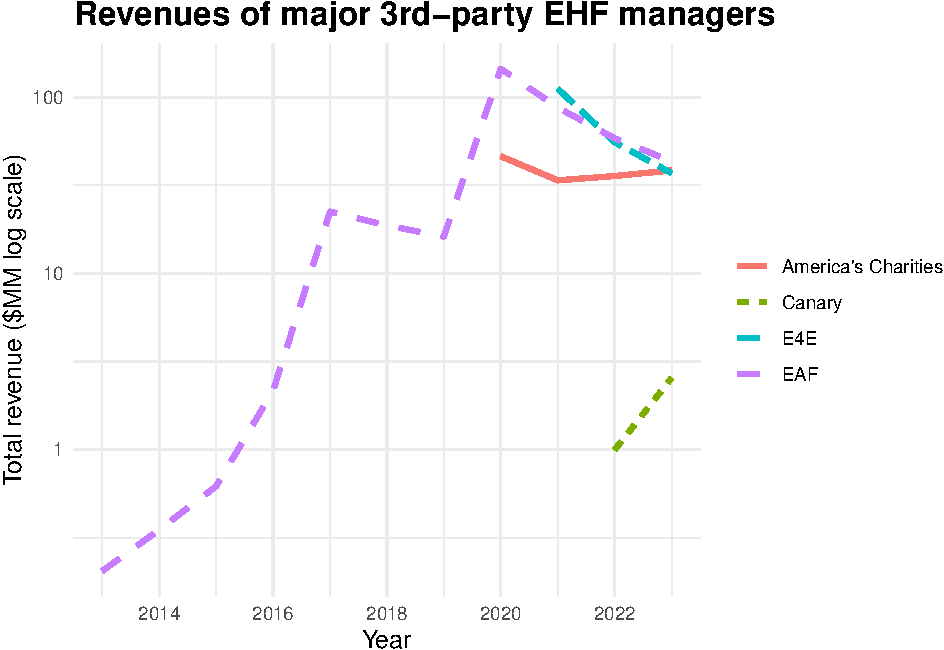
\includegraphics[width=0.5\linewidth]{EHF_Spring2025_files/figure-latex/fig-tpm-1} 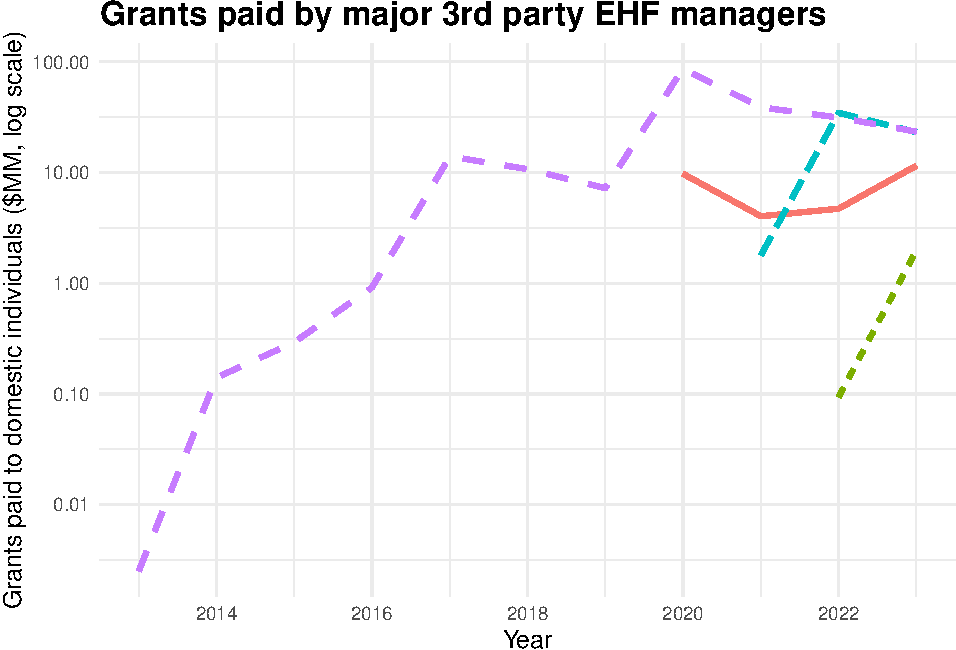
\includegraphics[width=0.5\linewidth]{EHF_Spring2025_files/figure-latex/fig-tpm-2} \caption{Revenue and grant activity at third-party EHF outsourcing organizations}\label{fig:fig-tpm}
\end{figure}

\begin{figure}
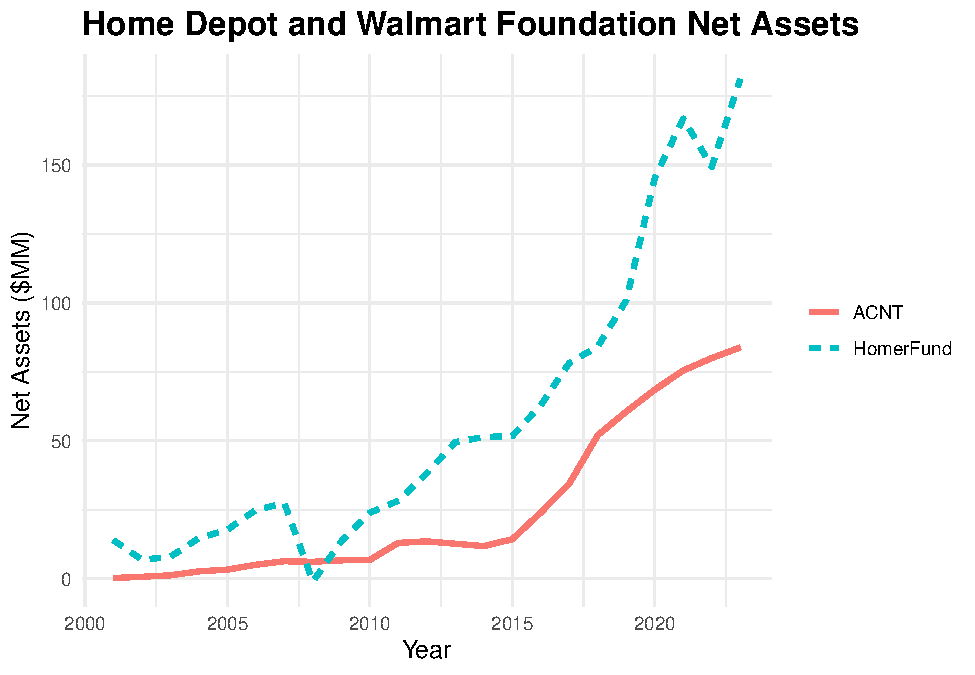
\includegraphics[width=0.5\linewidth]{EHF_Spring2025_files/figure-latex/fig-HfACNTcomps-1} 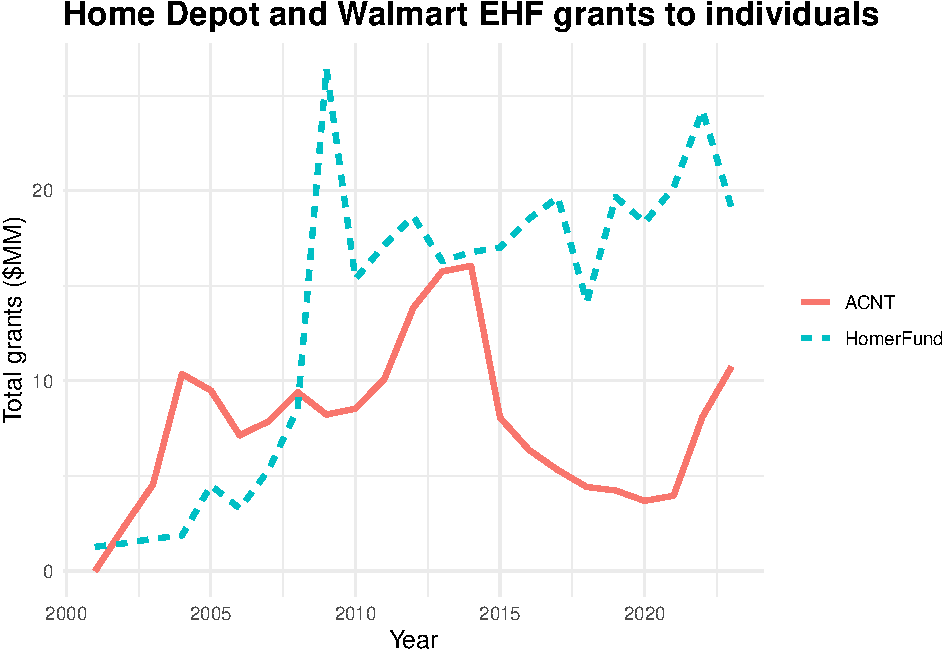
\includegraphics[width=0.5\linewidth]{EHF_Spring2025_files/figure-latex/fig-HfACNTcomps-2} \caption{EHF assets and grant activity at the Home Depot and Walmart.}\label{fig:fig-HfACNTcomps}
\end{figure}

Figure \ref{fig:fig-HfACNTcomps} zooms in on the Home Depot's Homer Fund (HF) and Walmart's Associates in Critical Need Trust (ACNT), two in-house EHF programs that we will examine in more detail. In the left panel I report net assets for both firms' nonprofit foundations.\footnote{For tax purposes, both HF and ACNT EHFs are part of the larger Home Depot and Walmart corporate foundations, respectively.} Both corporate charities show strong growth from 2010, but HF is operating at more than double the ACNT's size. The right panel looks at grants to domestic individuals, my preferred indicator of EHF activity.\footnote{The larger foundations typically focus on disbursing grants to other nonprofit and community organizations, as opposed to individuals. The HF website reports disbursing \$17 million in 2023 EHF grants whereas the Home Depot foundation 2023 IRS form 990 reports \$19.1 million in grants to individuals. No comparable information is available for the broader ACNT as opposed to the EHF Together Fund.} HF is making \$15-25 million in annual grants between 2008 and 2022 whereas ACNT typically disburses less than \$10 million, notwithstanding Walmart's much larger corporate presence. HF reports making a total of over \$267 million in grants to more than 183,000 individuals over its existence. ACNT claims to have disbursed over \$142 million over its existence to over 145,000 workers.

The comparisons above illustrate how EHF vary across firms in virtually all programmatic aspects including longevity, eligibility requirements, application procedures, grant generosity and frequency, funding structure, and even whether they are managed in-house or out-sourced to third parties like EAF. Although all EHFs have a mutual aid component, communication around the programs also varies in tone and intensity. Some firms, such as the Home Depot, aggressively promote their EHF programs. Messaging around these programs also varies, sometimes emphasizing charitable contributions social responsibility and sometimes framing the EHF as more of a job amenity or employment benefit.

Two critical features distinguish EHFs from other job amenities or employer-based insurance benefits, making EHFs particularly interesting. The first is their mutual aid nature. In EHFs, employers ask both corporate and frontline workers to donate their own money into a fund, with the goal of assisting fellow employees in need. Firms choose to sponsor an outreach and administrative apparatus to solicit and direct charitable contributions towards their own workforce. Second, EHFs are potentially accessible to hourly, part-time, or even contract workers. This sets EHFs apart from other benefits and protections that tend to accrue primarily to salaried and full-time workers. For example, Amazon.com restricted its EHF to ``Amazon Flex Delivery Partners, Delivery Service Partner Delivery Associates, Temporary Associates employed by eligible staffing agencies, and drivers of eligible line haul partners,'' i.e., non-standard, temporary contract labor.\footnote{As of 31 July 2022, Amazon no longer accepts applications to its EHF.} EAF updated its EHF program guidelines, recommending that employers ``include contractors, furloughed employees, and franchise employees'' in their EHF schemes (\citeproc{ref-employeeassistancefoundationDecadeAssistanceOffering2022}{Foundation 2022}).

\section{Mutual aid and welfare capitalism}\label{mutual-aid-and-welfare-capitalism}

Although EHFs are a relatively recent development, mutual aid is not. Industrialization uprooted workers from traditional sources of support while government social insurance programs were absent altogether. In the US, UK, and elsewhere, workers in an industry, region, or ethnic group routinely pooled their savings to assist one another in hard times (\citeproc{ref-beito_mutual_2000}{Beito 2000}; \citeproc{ref-glenn_understanding_2001}{Glenn 2001}; \citeproc{ref-dreyfus_labour_1993}{Dreyfus 1993}). Early mutual aid funds and friendly societies filled an otherwise unmet need. They both built on and deepened existing social connections, creating dense webs of obligation and formal organizational structures (\citeproc{ref-putnam_making_1994}{Putnam 1994}; \citeproc{ref-ismay_trust_2018}{Ismay 2018}). These organizations were precursors to modern trade unions (\citeproc{ref-webb_history_1920}{Webb and Webb 1920}; \citeproc{ref-bacharach_mutual_2018}{Bacharach, Bamberger, and Sonnenstuhl 2018}; \citeproc{ref-jarley_unions_2005}{Jarley 2005}), or even attempts to circumvent union repression (\citeproc{ref-morrisCriminalConspiracyEarly1937}{Morris 1937}).

Many unions built and continue to maintain emergency aid programs and insurance schemes to support, recruit, and retain members (\citeproc{ref-derickson_workers_1988}{Derickson 1988}; \citeproc{ref-dreyfus_labour_1993}{Dreyfus 1993}; \citeproc{ref-beito_mutual_2000}{Beito 2000}; \citeproc{ref-glenn_understanding_2001}{Glenn 2001}; \citeproc{ref-olson_logic_1965}{Olson 1965}; \citeproc{ref-hertel-fernandez_why_nodate}{Hertel-Fernandez and Porter 2021}). Other mutual aid arrangements grew into formal, state-regulated social insurance programs.

What distinguishes EHFs from past mutual aid programs are their employer-organized and firm-centered structure. Workers do not organize or direct the EHF, a worker need not donate in order to apply for benefits (unlike in a strictly mutualist arrangement), and EHFs are employer-specific. EHFs do not possess of organizational structures that build social connections or organizational skill among workers themselves. In some cases, workers must petition their direct supervisors to approve their application aid during a time of need.

EHFs hark back to the the era of ``welfare capitalism'' (\citeproc{ref-brandesAmericanWelfareCapitalism1976}{Brandes 1976}; \citeproc{ref-jacobyModernManorsWelfare1998}{Jacoby 1998}), when some employers provided health, education, entertainment, recreation, and even housing to workers in efforts to retain workers and forestall unionization. Some large industrial firms created employer-sponsored ``company unions'' that substituted for independent unions' social and mutual aid functions without any means of challenging management (\citeproc{ref-brandesAmericanWelfareCapitalism1976}{Brandes 1976}).\footnote{Such organizations were banned under the 1935 Wagner Act.} Even as with these efforts evident paternalism, they frequently represented considerable investments, shaping location and contours of production and the labor force and credibly signalling corporate commitments.

Employers continue to offer wages and other amenities to pre-preempt unionization, undermine unionization drives, and prevent workers from defecting to unionized competitors Taschereau-Dumouchel (\citeproc{ref-taschereau-dumouchelUnionThreat2020}{2020}). But with actual union power declining, employers face reduced incentives to make the long term investments of the past.
In short, EHFs are novel, tax-incentivized initiatives that echo past organizational forms. They may have effects on workers that also blend those from mutual aid and welfare capitalism.

\subsection{Why EHFs?}\label{why-ehfs}

There are are several (non-exclusive) reasons why employers might develop EHFs, each of which has implications for how these programs might affect the workforce. Although I do not attempt to document or explain variation in EHFs across firms, I drawing on semi-structured interviews with EHF practitioners to generate hypotheses about how these programs emerge and connect to workers' politically and economically important attitudes and behaviors around job attachment, unionization, and social insurance.\footnote{Selected quotations from interviews appear in Appendix \ref{app-interviews}.}

\subsubsection{Spontaneous initiatives from executives}\label{spontaneous-initiatives-from-executives}

Some EHFs appear to be the result of spontaneous initiatives from executives, often in response to a major natural disaster affecting a region closely connected to the firm and its employees.\footnote{Disaster aid and social insurance are closely linked in the US (\citeproc{ref-landis_fate_1999}{Landis 1999}).} Based on interviews, this often stemmed from frustration with the slow or uneven aid emerging from government.

Even before COVID-19, there was plenty of evidence that the existing social insurance and welfare systems were stigmatizing, encumbered with numerous ``administrative burdens'' (\citeproc{ref-herd_administrative_2019}{Herd and Moynihan 2019}), and straining to deliver to those in need. Several informants suggested that EHFs may present a private, partial complement to a weakening or slow public system. By locating mutual aid programs in the firm, program participation might be higher and the EHF can benefit from corporate resources. Applying for an EHF grant may be easier or less stigmatizing than applying for government assistance and the turn around time for benefits could be much faster in times of acute need.\footnote{The Home Depot claims that grants are processed within 7 business days of application receipt, far faster than welfare or unemployment benefits, which also require waiting periods in many states.}

\subsubsection{Communicating corporate culture and building attachment}\label{communicating-corporate-culture-and-building-attachment}

Reports from practitioners and author interviews with EHF managers suggest that EHFs send important signals about the employer's corporate culture, building common knowledge about corporate values and commitments. The Home Depot, for example, published a detailed set of suggested donations to the Homer Fund, based on salary tiers (see appendix figure \ref{fig:fig-sugdon}) . Author interviews with EHF practitioners corroborated the programs' perceived value in communicating corporate values and instilling corporate culture (see Appendix \ref{app-interviews}).

This can be valuable to employers. There is growing evidence that strong corporate cultures that signal mutual interdependence and care can attract similarly-minded workers and increase positive disposition toward the employer and coworkers. These, in turn, can increase productivity and decrease turnover (\citeproc{ref-kampkotter_employee_2020}{Kampkötter, Petters, and Sliwka 2020}; \citeproc{ref-lin_modeling_2010}{Lin 2010}). Similarly, mutual aid programs might be a mechanism whereby workers from diverse backgrounds and spread all over the country come to see their fates as intertwined with one another and the firm, developing a sort of ``community of fate'' (\citeproc{ref-ahlquist_interest_2013}{Ahlquist and Levi 2013}; \citeproc{ref-ismay_trust_2018}{Ismay 2018}). Recent research on corporate CSR campaigns reinforces this connection. Signals about corporate charity and other pro-social activities can increase worker retention (\citeproc{ref-bodeCorporateSocialInitiatives2015}{Bode, Singh, and Rogan 2015}) and even increase uncompensated worker effort in gig-economy jobs (\citeproc{ref-burbanoGettingGigWorkers2021}{Burbano 2021}). In other words, information about EHFs may enhance workers' subjective attachment to the employer and possibly one another. The social and psychological mechanisms involved remain contested.

But the nature of work and labor contracting are changing (\citeproc{ref-weil_fissured_2014}{Weil 2014}; \citeproc{ref-ahlquist_research_2018}{Ahlquist 2018}), with increasing prevalence of precarious and supplier-like ``independent contractor'' relationships. In the US, many labor protections and social insurance benefits do not accrue to workers in such ``nonstandard'' employment relationships nor are these workers generally eligible for employer-provided benefits such as health insurance and paid time off. This may save some labor-related costs in the near term, but these precarious contractor relationships have additional costs. Workers in non-standard contracting arrangements may be less loyal to the firm and less motivated to exert additional effort and therefore less productive. Nonstandard work may also pose a threat to the corporate brand, to the extent that the broader public finds such arrangements unfair or exploitative. EHFs could be a way to signal corporate values and culture while building an approximation to worker community. EHFs may also represent one avenue by which firms can direct some benefits to their workers--perhaps improving morale and blunting public criticism--without jeopardizing the savings that make non-standard labor contracting attractive. Some EHFs---notably Amazon's short-lived initiative---are explicitly aimed at part-time and contract workers. But others only consider directly employed (``W-2'') workers and sometimes impose a minimum tenure requirement for grant eligibility.

\subsubsection{``ESG'' concerns}\label{esg-concerns}

There are other ends that EHFs might serve alongside charitable motivations or team-building functions. One is investor relations (\citeproc{ref-godfreyRelationshipCorporateSocial2009}{Godfrey, Merrill, and Hansen 2009}). ``Environment, Social, and Governance'' (ESG) became something of a corporate fad in the late 2010s, spawning numerous mutual funds and other investment vehicles that claim to channel resources toward companies that meet particular standards for sustainability, stakeholder respect, and corporate governance. This, in turn, has created a whole slew of ESG ratings, with various levels of transparency and disclosure. Whether EHFs succeed in is unclear. But several major retailers, including the Home Depot, Kohl's, and Walmart aggressively promoted their EHFs in their ESG reports (\citeproc{ref-THD_ESG_2022}{The Home Depot 2023b}). Author interviews with EHF professionals confirm that some of the recent interest in EHFs stems from the hope that EHF programs will help with investor relations and ``count'' in the ``S'' bucket when large investors and fund managers evaluate a company's ESG performance.\footnote{Some also mention that EHFs could count in the ``E'' bucket, as a form of natural disaster planning.} But informants also indicate that ESG/investor relations is not the core motivation (see Appendix \ref{app-interviews}).

\subsubsection{Union avoidance}\label{union-avoidance}

Related to investor relations is union avoidance. Unionization remains low in the United States but interest in labor unions is at historically high levels (\citeproc{ref-Gallup_unions_2022}{McCarthy 2022}; \citeproc{ref-WERNsurvey2023}{Workers Empowerment Research Network 2023}; \citeproc{ref-kochan_worker_2019}{Kochan et al. 2019}). High profile unionization drives have been a regular occurrence in the traditionally hard-to-organize retail sector over the last decade. Employer resistance remains strong, with firms employing a variety of tactics--legal and otherwise--to thwart unionization efforts.

EHFs may both increase loyalty and provide an amenity that substitutes for those typically associated with unions. EHFs may even appear more desirable than union mutual aid programs, insofar as workers are not obligated to contribute in order to apply for EHF benefits and EHFs may receive subsidies in the form of corporate and executive donations, something union funds rarely see. EHFs also take on a form and rhetoric that may connect with the same ``social custom'' or solidaristic motivations that support union membership (\citeproc{ref-akerlof_theory_1980}{Akerlof 1980}; \citeproc{ref-naylor_economic_1993}{Naylor and Cripps 1993}). As such, employers could point to EHFs as a union-like workplace benefit as part of a broader union avoidance strategy. Whether this strategy might plausibly work is something this paper seeks to determine.

The union substitution hypothesis also has an echo in the literature on support for the welfare state. There is now a growing body of scholarship arguing that government welfare programs and private resources substitute for one another (\citeproc{ref-beito_mutual_2000}{Beito 2000}; \citeproc{ref-yeo_working_1979}{Yeo 1979}; \citeproc{ref-wiedemann_how_2022}{Wiedemann 2022}). Public programs often step in when private mutual aid or insurance pools collapse. For example, the famous ``Ghent system,'' in which unions administer government-mandated unemployment insurance, arose out of the repeated collapse of various privately-organized welfare and mutual aid pools (\citeproc{ref-socialsecurityadministrationSocialSecurityHistory2023}{Administration 2023}; \citeproc{ref-western_1997}{Western 1997}). Conversely, increases in private resources, private insurance, or employer-provided benefits can crowd out support for government programs (\citeproc{ref-ansell_political_2014}{Ansell 2014}; \citeproc{ref-busemeyer_welfare_2020}{Busemeyer and Iversen 2020}; \citeproc{ref-rosner_struggle_2003}{Rosner and Markowitz 2003}; \citeproc{ref-hacker_insecure_2013}{Hacker, Rehm, and Schlesinger 2013}; \citeproc{ref-zhu_policy_2015}{Zhu and Lipsmeyer 2015}) and possibly unions (\citeproc{ref-bacharach_mutual_2018}{Bacharach, Bamberger, and Sonnenstuhl 2018}; \citeproc{ref-quadagno_transformation_1988}{Quadagno 1988}; \citeproc{ref-neumannWhereHaveAll1984}{Neumann and Rissman 1984}). Increased awareness of EHFs could blunt support for social insurance, regulation of non-standard work, or even government aid programs in times of emergency (e.g., COVID-19). Again, this paper seeks to determine whether we can observe this effect among workers exposed to EHF information.

Interviews with practitioners and EHF managers were less clear on these points. Informants did not volunteer any comments about unions and were reluctant to discuss worker participation in EHFs more generally. When asked about whether and how their EHF programs were designed to connect with public services and social welfare benefits, informants demurred or viewed EHFs as complimentary to public assistance.

\subsubsection{Cost effectiveness}\label{cost-effectiveness}

EHFs are cheap. Overhead is low and operations can be outsourced to third parties. Monetary commitments from the employer are discretionary and grants awards can be adjusted at will to match resources, with little fanfare or oversight. Funds come, in part, from workers themselves and contributions to the fund, especially from executives and higher-paid corporate employees, are treated as tax-deductible charitable donations. Relatively minor costs and low risks likely contribute to the remarkable spread of EHFs in recent years.

Nevertheless, firm-based mutual aid arrangements could have other drawbacks, depending on how the program is run. From the worker's perspective, an EHF is not ``portable.'' Should the worker leave her job at a specific firm, her access to the emergency grant goes with it. Emergency relief might vanish when it is most needed, enhancing management's leverage over workers at moments of vulnerability and increasing resentment. As a specific example, until 2020, workers seeking emergency grants from the HF had to first receive ``support'' from their supervisor or a salaried manager. EHFs may end up being \emph{more} stigmatizing than public services, to the extent that a worker's hardship or need is now visible to managers or co-workers. EHF benefits are more akin to charity one must petition for than a benefit one is owed as a result of past contributions (\citeproc{ref-fothergill_stigma_2003}{Fothergill 2003}; \citeproc{ref-parsell_clarke_2022}{Parsell and Clarke 2022}; \citeproc{ref-williamson_stigma_1974}{Williamson 1974}). Finally, EHFs may backfire. Many of the firms that offer EHFs are not known for good wages or generous benefits. There has been some predictable criticism: why is a multibillion dollar company trying to raise money from its own low-paid workforce? Why not just pay workers better wages and improve benefits? Why not support public policies that would improve everyone's ability to weather hardships? As these programs grow, these criticisms will surely mount and could present a threat to brands.

Again, interviews with practitioners regularly pointed to EHF's low cost and flexibility as reasons for their popularity and growth. There was also concern with program management to minimize any blowback from workers.

\subsection{Research goals}\label{research-goals}

There are important scope conditions and points of clarification. First, there is a chicken-and-egg problem. On the one hand, cross-firm variation in EHFs is important for understanding the programs' possible effects. But we want to document EHF \emph{effects} to understand why firms might create these programs and how they might differ. Because EHFs are ostensibly targeted at workers and for reasons of tractability, this paper concentrates on how workers interact with EHFs. Exploring cross-firm variation will require a different research design.

In a similar vein, I am interested in how a company's broad workforce interact with an EHF, \emph{not} the effect of EHF grant receipt on individuals in need. This is for reasons of theoretical interest as well as tractability. A small proportion of a firm's employees is ever likely to qualify and apply for EHF assistance.\footnote{Based on estimates from Study 1, 27\% of retail workers may have experienced a potential ``qualifying event'' in the last year.} Not only does this make it quite difficult to credibly compare grant recipients with non-recipients, but, more importantly, it suggests that the effects of these programs are likely to spillover more broadly.

Third, we know very little about these programs, meaning there are important unanswered descriptive questions. What proportion of workers are even aware of their employer's EHF? Are they aware of these programs at other employers in their industry? What proportion have engaged with the EHF (contributed, applied, received a grant)? What are the predictors of EHF awareness and engagement? Of those who experienced a qualifying event, how many applied for EHF support? How much do workers value EHFs relative to other job amenities?

Fourth, in the absence of basic descriptive information about EHFs, we do not yet have a convincing empirical strategy for identifying the causal effects of EHF introduction on the workers at a specific firm or in an entire industry. Instead, I propose a tractable, individual-focused approach using experiments embedded in surveys to manipulate the information and salience of EHFs in the minds of respondents. I am therefore also careful to account for whether a respondent was aware of the EHF program (i.e., ``pre-exposed'') prior to the survey.

Fifth: the reasons a firm sponsors an EHF are distinct from any effects an EHF may have. Executives could have goals for the EHF that they fail to achieve. EHFs likely go unnoticed or unremembered most of the time. EHFs could also have unplanned consequences. The research design in this paper speaks to whether realistic informational campaigns \emph{could} affect worker attitudes, for example by calling attention to an EHF as part of a worker on-boarding process or anti-unionization strategy.

Beyond the descriptive quantities just outlined, the survey experiments described below will speak to the following hypotheses:

\begin{enumerate}
\def\labelenumi{\arabic{enumi}.}
\tightlist
\item
  Improving worker financial stability in the face of unexpected emergencies is a stated goal for EHFs. Prompting workers with information about their employer's EHF will improve their perceived financial security, as measured by reported ability to meet a \$400 emergency expense.
\item
  EHFs may improve disposition toward co-workers by providing evidence that the co-workers are ``types'' who who contribute to group projects or care about the welfare of others. The employer's reputation may also benefit, as the organization who set up the program and hires ``good'' people. Prompting workers with information about their employer's EHF will increase a worker's positive disposition toward co-workers and towards the employer while reducing quit intentions.
\item
  EHF may be viewed as ``private insurance'', which could dampen support for unionization and social insurance. Prompting workers with information about their employer's EHF will reduce workers' willingness to vote for unionization and reduce stated support for government aid programs for unemployment or emergencies.
\item
  Direct emotional appeals, especially for people like oneself increase the willingness to contribute to charitable causes (\citeproc{ref-andreoniPowerAskingHow2011}{Andreoni and Rao 2011}). Direct appeals around the EHF will increase workers' willingness to donate to the EHF.
\end{enumerate}

\section{Study 1}\label{study-1}

In study 1, I set out to answer basic descriptive questions: are workers aware of EHFs? How accurate is their knowledge? How attractive do they find EHFs, relative to other job amenities? I concentrate on the retail industry, which employed more than 16 million Americans in 2024. Retail is known for low wages, poor benefits, high turnover, and several high-profile recent unionization drives. EHFs are widespread in the industry and there are several very large employers, making a survey strategy feasible.

I fielded an original survey using the Cloud Research incentivized panel, targeting US respondents 18+ employed in retail.\footnote{In the pre-registered study, we planned a survey of Costco workers, as Costco is the only major retailer without an EHF. It proved impossible to recruit a sample of Costco workers, so I turned to a study of general retail workers. Measurement and analysis of the survey follows the pre-registered plan.} Of those targeted, only respondents with US IP addresses, who passed a screening question confirming employment in the retail industry, and who successfully passed two different attention check questions were allowed to complete the survey. Respondents with duplicate IP addresses reporting identical demographic values were also excluded. The survey was in the field from February 12 - 22, 2025 and produced 1008 valid responses. Using the 2024 ACS-reported demographics for US adults working in retail, we constructed post-stratification weights based on gender, race, and education. All descriptive quantities below represent weighted calculations.

\subsection{Worker awareness}\label{worker-awareness}

We asked respondents which of a list of benefits and programs they had at their current retail job. The EHF response on this list is ``emergency cash support.'' We find that 23\% (se = 1\%) report that their current employer offers emergency cash support and 31\% (se = 2\%) said that they had heard of EHF programs prior to taking the survey. By way of comparison, in a separate, Fall 2022 survey of frontline workers in five industries (including retail), we asked respondents about programs and benefits available at their main job using the same method (\citeproc{ref-AGT_youngworkers}{Ahlquist, Grumbach, and Thai 2023}; \citeproc{ref-WERNsurvey2023}{Workers Empowerment Research Network 2023}). Twelve percent (12\%) of that sample and 13\% of retail workers reported that their employer had an emergency cash grant program. Note that we are unable to confirm the accuracy of respondents' reports about their employers' EHFs, so these quantities represent perceptions only.

To evaluate the breadth and accuracy of retail workers' EHF knowledge, I presented respondents with a definition of EHF programs.\footnote{All respondents in Study 1 answered the following question before responding to questions about : ``Some companies offer their employees programs called''Employee Hardship Funds.'' Employee Hardship Funds provide emergency cash to a company's workers if they face unexpected financial hardships, such as a house or apartment fire. The emergency money from the Employee Hardship Fund is not a loan and does not have to be repaid. The money in the fund comes directly from donations from the company's own workers. Before taking this survey, had you ever heard of Employee Hardship Funds?''} A subsequent question asked them to state whether each of six large retail employers had an EHF.\footnote{The employers were Costco (no), Disney (yes), Home Depot (yes), Kohl's (yes), Starbucks (yes), Walmart (yes).} Figure \ref{fig:fig-genpop-beliefs} displays the distribution of responses across all firms separately for workers who claim to currently have a job with an EHF versus those that do not.

\begin{figure}
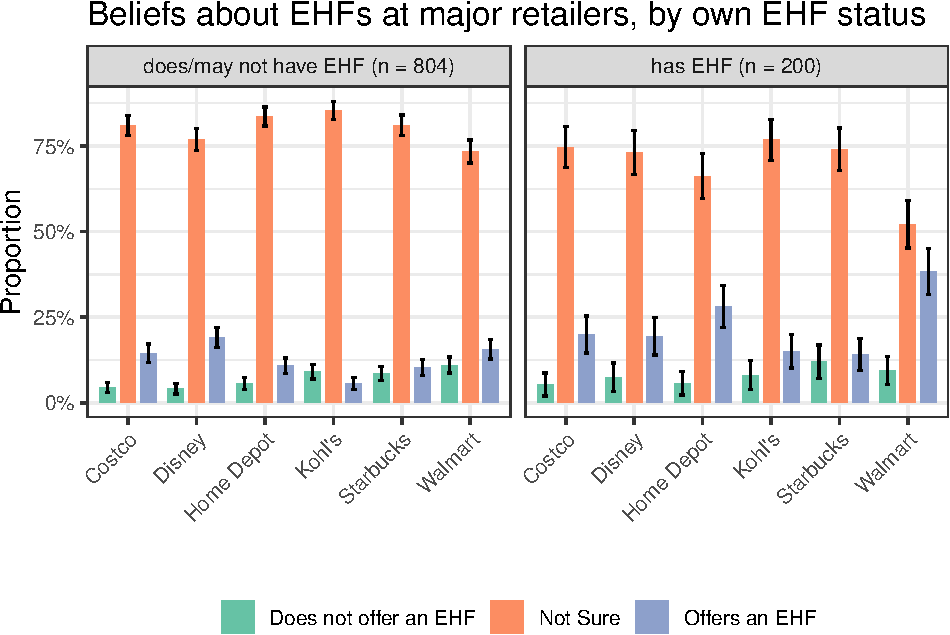
\includegraphics[width=0.8\linewidth]{EHF_Spring2025_files/figure-latex/fig-genpop-beliefs-1} \caption{Worker beliefs about EHFs at major US retailers}\label{fig:fig-genpop-beliefs}
\end{figure}

Regardless of current EHF exposure, large majorities of respondents admitted their ignorance as to which retail employers offered EHF programs. Those who made choices about which employers offered EHFs did worse, on average, than pure chance guessing. Nevertheless, respondents who report an EHF at their current job are less likely to express ignorance and much more likely to offer the (correct) EHF response for the Home Depot and, especially, Walmart. Overall, these findings suggest that retail workers' EHF awareness is superficial at best. But there is also some indication that Walmart and Home Depot are better known and recognized as having these programs.

\subsection{Interest and preferences over EHFs}\label{interest-and-preferences-over-ehfs}

Notwithstanding their limited awareness of existing EHF programs, respondents were remarkably supportive of EHFs after they were explained, preferring a program in which workers have some voice. When asked about a willingness to donate to the EHF, 82\% would donate, with a modal response of a ``regular donation less than \$20''. Figure \ref{fig:fig-genpop-support} displays levels of support for an existing or hypothetical EHF. In both cases, large majorities show ``extreme'' support. Workers already exposed to EHFs showed even stronger support than those asked to consider a hypothetical program, with 63\% ``extremely'' supportive against 57\%.

\begin{figure}
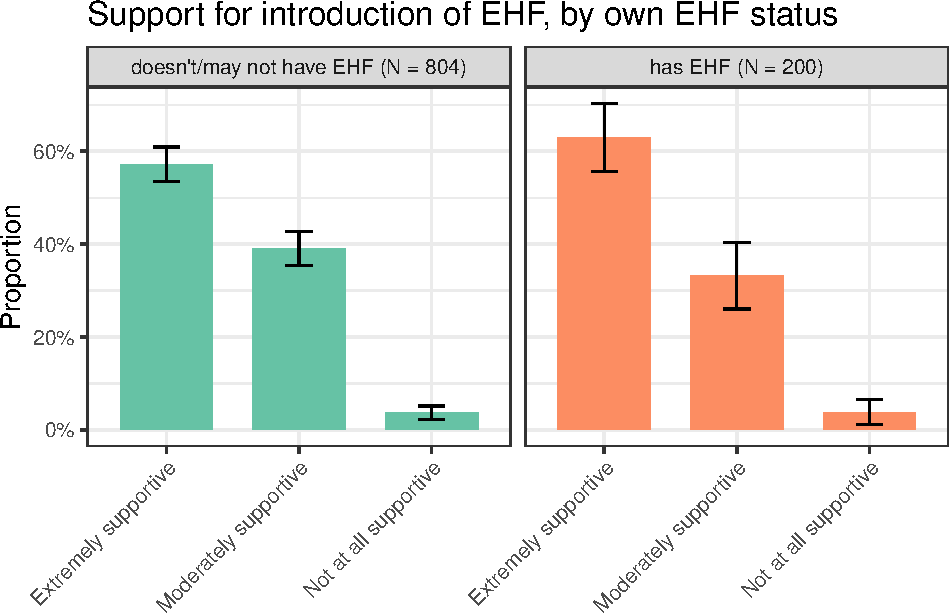
\includegraphics[width=0.8\linewidth]{EHF_Spring2025_files/figure-latex/fig-genpop-support-1} \caption{Support for creating or maintaining  an EHF}\label{fig:fig-genpop-support}
\end{figure}

I went on to ask respondents to consider a hypothetical job with another retailer that paid the same wages as their current job, has a 10 minute longer commute, but better amenities. I asked how seriously they would consider the new job depending on which amenity was better. Figure \ref{fig:fig-genpop-prefs} displays the responses. Among the amenities offered, ``emergency cash offered during hard times'' was second only to paid time off in terms of the proportion of respondents saying they would take the new job ``very seriously.'' EHF programs were notably more attractive to workers than parental leave or union representation.

\begin{figure}
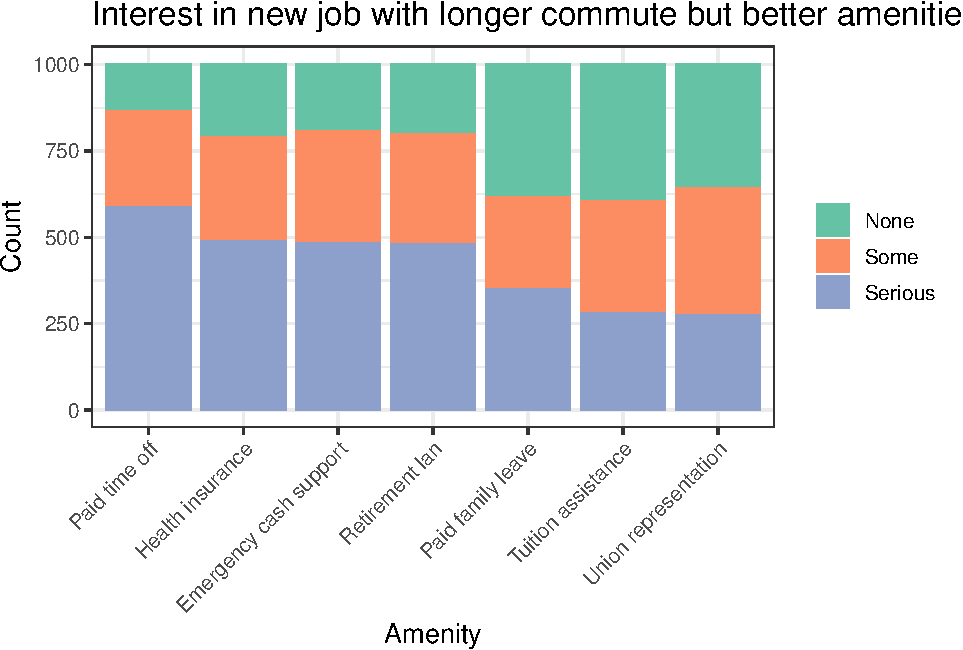
\includegraphics[width=0.8\linewidth]{EHF_Spring2025_files/figure-latex/fig-genpop-prefs-1} \caption{Preferences over job amenities}\label{fig:fig-genpop-prefs}
\end{figure}

Finally, I asked respondents who did not report having an EHF how much control workers \emph{should} have if their employer launched an EHF program. As displayed in Figure \ref{fig:fig-genpop-control}, large majorities prefer that workers have a voice in running the fund. As an empirical matter, I have not been able to find a single EHF in which there is a representative of frontline workers involved in the EHF.

\begin{figure}
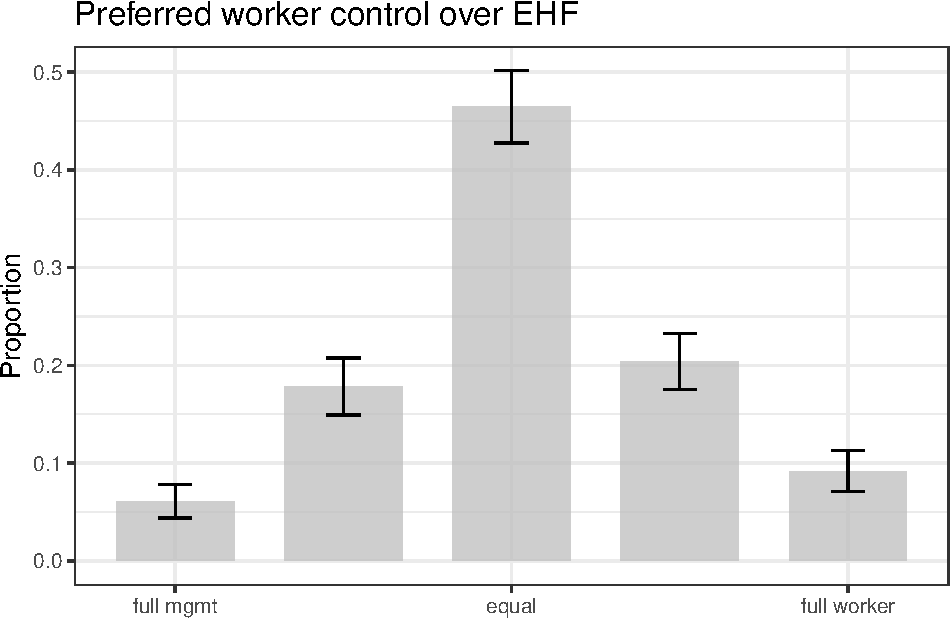
\includegraphics[width=0.8\linewidth]{EHF_Spring2025_files/figure-latex/fig-genpop-control-1} \caption{Preferences worker voice in the EHF}\label{fig:fig-genpop-control}
\end{figure}

Study 1 suggests that, although they are not widely known or understood, EHFs receive strong support and can be attractive amenities to retail workers.

\section{Study 2}\label{study-2}

\subsection{Case selection}\label{case-selection}

In Study 2 I seek to answer more detailed questions about EHF awareness and engagement as well as conduct meaningful survey-based experiments. Study 2 focuses on one large US retailer, The Home Depot. The Home Depot operates nationwide and reports 418,000 ``associates'' in the US in 2022, making it feasible to recruit a sizable survey sample (\citeproc{ref-THD_AR_2022}{The Home Depot 2023a}). The Home Depot's EHF--The Homer Fund--is managed in-house and been in continuous operation since 1999. HF is among the most generous EHFs, with a maximum grant amount of \$10,000 and the ability to apply repeatedly. The HF is sizable, reporting disbursements of \$21.2 million to over 12,000 workers in the 2022 fiscal year (\citeproc{ref-THD_ESG_2022}{The Home Depot 2023b}). The fund claims that it has disbursed \$230 million to 164,000 employees between 1999 and 2022. Most importantly for my purposes, The Home Depot aggressively promotes the program internally to solicit worker donations and engagement the fund. The HF has a dedicated website and YouTube channel with numerous professional-quality testimonial videos, along with active social media accounts aimed at workers. The Home Depot runs regular donation drives in which different stores compete with one another to generate participation and donation dollars for the EHF. The HF prides itself on worker participation; their website states that a ``majority of contributions'' come from ``associates.''\footnote{\url{https://corporate.homedepot.com/page/homer-fund-0}}

The Home Depot is clearly not representative of all firms or even all firms that maintain EHFs. It is larger and puts more effort and resources behind its EHF, having done so for longer than almost any other firm. I therefore view the Home Depot as a extreme case. Interviews with EHF practitioners suggest that worker awareness at the Home Depot likely approaches the upper bound of what is achievable among US retail employers.

\subsection{The sample and survey}\label{the-sample-and-survey}

Constructing a matched worker-employer survey sample is quite challenging. I follow Schneider and Harknett (\citeproc{ref-schneider_whats_2019}{2019}) and recruit participants through ads on the Facebook and Instagram platforms targeted at users 18 and older with Facebook-reported status as Home Depot employees. Those completing the survey were offered entry into a raffle for a free iPad Mini. Schneider and Harknett (\citeproc{ref-schneider_whats_2019}{2019}) show that this strategy has considerable promise, providing accurate estimates of the employee population in the retail industry. But the Facebook strategy has the primary drawback of sample selection. To some degree this is unavoidable. But to partially mitigate selection concerns, I follow Schneider and Harknett (\citeproc{ref-schneider_whats_2019}{2019}) and construct raking weights using the Facebook-reported gender and age distributions for Facebook/Instagram users who report employment at the Home Depot. Other work shows that Facebook-reported age and gender appear quite accurate (\citeproc{ref-grow_is_nodate}{Grow et al. forthcoming}). I use raking weights when reporting descriptive quantities, but I use the unweighted data when analyzing the survey experiment.

Survey recruitment occurred between 7 September and 15 October 2021. We ultimately received 515 complete responses who also passed an attention check and a screening question confirming their Home Depot employment status. Discussion of the sample as well as summary statistics for all variables by treatment condition appear in Appendices \ref{app-survsum-uw} and \ref{app-survsum-w}.

\subsection{HF awareness and engagement}\label{hf-awareness-and-engagement}

We first look at Home Depot workers' awareness of and engagement with their employer's EHF.

Our preferred measure of awareness comes from a list of eight work-related benefits or programs presented to respondents.\footnote{I discuss two other indicators of awareness and compare them with the preferred ``list'' measure in Appendix \ref{app-HFaware}.} They were asked to select all available to ``workers like you.'' Among the possible programs was ``cash grants to help in times of emergency.'' The proportion of respondents selecting this answer provides a measure for EHF awareness available for all survey respondents without contaminating the later survey experiment. I estimate that 61\% (se = 2\%) were aware of a cash grant program.

As indicators of engagement, we asked whether respondents had donated to, applied to, received money from, and know personally someone who has received money from the EHF.\footnote{The donation and grant receipt questions were asked of all respondents while the applied and ``know someone'' questions were asked only of treatment group respondents, post-treatment.} A remarkable 73.2\% (se = 2.2\%) of respondents reported that they had donated. Roughly 30\% of the respondents indicating donation fail to identify emergency cash grants as a benefit their employer offers. We find that 54.1\% (se = 3\%) claim to know someone who has gotten money from the program. I consider this a remarkably high number.

Application and grant receipt estimates are also quite high. Among our respondents we find that, respectively, 21\% and 13\% applied for and received EHF grants. Survey self-reports indicate that 29\% experienced an event in the last 12 months that would make them potentially eligible for and HF grant. Of that group, 28\% applied to the HF.

Compared to the general retail population in Study 1, EHF awareness among Home Depot workers is quite high. Consistent with the messaging around the Homer Fund donation drives, it appears that Home Depot workers are aware of a charitable endeavor that relates to their coworkers. But worker awareness of the program's \emph{benefit} function appears relatively thin.

To explore the predictors of EHF awareness and engagement, we fit weighted logistic regression models, including age, gender, tenure at the firm\footnote{In measuring firm tenure, respondents could choose among \{less than 6 months, 6-12 months, 1-2 years, 2-3 years, 3+ years\}. I enter this variable in minimum months of tenure, \{0,6,12,24,36\} in the regression models for ease of exposition. Entering as dummy variables or ordered categories does not affect inference or appreciably improve model fit.}, race (white/nonwhite), and education (college/no college) as covariates. We also include indicators for whether the Home Depot job is the respondent's main job, whether this job paid on an hourly basis, and whether it's full time. Coefficient estimates and standard errors appear in Table \ref{tab:awareness-model}.

Once we condition on multiple covariates, tenure at the Home Depot is the only predictor with a relatively precisely estimated relationship across all indicators of awareness and engagement in the expected positive direction. Full-time workers are also more likely to report awareness of a cash grant program but these estimates are less-precise. Tenure and full-time status are closely related: over 72\% of the respondents with tenure over 3 years work full time against less than 50\% for those with less than 3 years at the firm. Other worker attributes appear to have little relationship with EHF awareness. Older workers are slightly more likely to donate and less likely to receive grants whereas men are less likely to apply to the EHF or know other recipients.

\begin{table}
\centering
\caption{\label{tab:awareness-model}Weighted logistic regression of Home Depot EHF awareness and engagement \label{tab:awareness-model}}
\centering
\begin{threeparttable}
\begin{tabular}[t]{lccccc}
\toprule
  & awareness & know recipient & applied & received & donated\\
\midrule
age & \num{-0.007} & \num{0.016} & \num{0.022}* & \num{0.015} & \num{0.021}*\\
 & (\num{0.006}) & (\num{0.009}) & (\num{0.009}) & (\num{0.009}) & (\num{0.010})\\
male & \num{-0.162} & \num{-1.009}** & \num{-0.928}** & \num{-0.517} & \num{-0.210}\\
 & (\num{0.211}) & (\num{0.300}) & (\num{0.332}) & (\num{0.290}) & (\num{0.315})\\
main job & \num{0.013} & \num{0.006} & \num{0.326} & \num{0.719} & \num{-0.288}\\
 & (\num{0.388}) & (\num{0.614}) & (\num{0.611}) & (\num{0.688}) & (\num{0.590})\\
tenure & \num{0.026}** & \num{0.078}** & \num{0.076}** & \num{0.117}** & \num{0.121}**\\
 & (\num{0.009}) & (\num{0.013}) & (\num{0.021}) & (\num{0.027}) & (\num{0.013})\\
nonwhite & \num{-0.231} & \num{-0.187} & \num{0.091} & \num{0.100} & \num{0.231}\\
 & (\num{0.248}) & (\num{0.365}) & (\num{0.375}) & (\num{0.377}) & (\num{0.351})\\
full time & \num{0.425} & \num{0.363} & \num{0.248} & \num{-0.090} & \num{0.386}\\
 & (\num{0.238}) & (\num{0.331}) & (\num{0.412}) & (\num{0.359}) & (\num{0.337})\\
hourly & \num{-0.605} & \num{-0.975} & \num{1.125} & \num{-0.830} & \num{0.460}\\
 & (\num{0.669}) & (\num{1.017}) & (\num{0.871}) & (\num{0.635}) & (\num{1.117})\\
college & \num{0.387} & \num{0.257} & \num{-0.698} & \num{0.121} & \num{0.450}\\
 & (\num{0.282}) & (\num{0.352}) & (\num{0.478}) & (\num{0.361}) & (\num{0.526})\\
\midrule
$N$ & \num{509} & \num{346} & \num{347} & \num{509} & \num{508}\\
AIC & \num{671} & \num{393} & \num{315} & \num{341} & \num{385}\\
\bottomrule
\end{tabular}
\begin{tablenotes}
\item * p $<$ 0.05, ** p $<$ 0.01 Standard errors in parentheses.
\end{tablenotes}
\end{threeparttable}
\end{table}

\subsection{EHF experiment}\label{ehf-experiment}

I included a randomized experiment in the survey. Survey experiments are particularly useful here for two reasons. First, the survey experiment provides better control and more credible causal estimates than those relying on comparisons of observational data. Second, the survey experiment retains internal validity even in the face of questions about selection into the survey, survey weighting, or selection into EHF programs.

In the experiment were a control condition and two treatment arms, referred to as the \emph{text} and \emph{video} treatments, respectively. Respondents in the control arm saw no prompt or mention of the EHF. Those in the text treatment saw the following statement about their employer's EHF:

\begin{quote}
Your employer, The Home Depot, maintains a program called the Homer Fund. The Homer Fund combines donations from workers like you with money from The Home Depot corporation. The Homer Fund uses this money to offer cash grants of up to \$10,000 to Home Depot employees in times of unexpected financial hardship like a natural disaster, illness, or death in the family.
\end{quote}

A brief, neutral text prompt does not reflect how employers actually communicate with their employees. I take advantage of the Home Depot's existing promotion of the HF. The HF posts professionally-produced video testimonials from purported HF recipients on the HF website and YouTube channel. Respondents in the video treatment were presented with one of these testimonial videos (2:41 in length) before answering the same set of questions. Figure \ref{fig:fig-ray} displays a screen shot of the video treatment.\footnote{The video can be found here: \url{https://www.youtube.com/watch?v=qF-HBoySMe} and here: \url{https://corporate.homedepot.com/news/foundation-and-community/homer-fund-celebrates-20-years-giving-rays-story}. The summary text appearing on the Home Depot website is: ``When Ray, a retired Army veteran and proud Home Depot associate, fell severely ill, his family needed help covering expenses such as food and gas. With the help the Homer Fund and his fellow associates' generosity, he and his family were able to recover. The Homer Fund, a nonprofit exclusively for Home Depot associates, celebrates 20 years of giving in 2019. Established by our co-founders Bernie Marcus, Arthur Blank and Ken Langone, it has awarded \$176 million to more than 138,000 Home Depot families facing unforeseen hardships. For Ray and his family, The Fund's help came at a critical time. Ray spent six weeks in an induced coma. The Homer Fund stepped in to help his family secure necessities so they could focus their energy on Ray's recovery. The Fund's impact on Ray's family reminded him of the comradery of his Army days. `You know you have a brother and sister to your left or to your right. And you look out for them and they look out for you,' Ray says.'' This text was not presented to survey respondents, but is presented here to provide a summary of video contents.} Immediately following the experimental treatment, I asked a series of questions designed to measure respondents' subjective financial well-being, attachment to co-workers, attachment to their employer, willingness for vote for unionization, and support government-provided unemployment insurance, childcare, and old-age pensions.

\begin{figure}
\includegraphics[width=0.6\linewidth]{plots/RaysStory} \caption{Image of the video treatment}\label{fig:fig-ray}
\end{figure}

\subsubsection{Analytic approach}\label{analytic-approach}

I am primarily interested in the average treatment effects for each of the two EHF treatments relative to control for each of the outcome variables. I present graphical displays as well as regression-based estimates. We then look for potential differences in treatment effects, depending on whether the respondent was aware of the EHF program before the survey experiment. This latter quantity was not part of the initial pre-analysis plan so I explain its inclusion before moving on.

\subsubsection{Acccounting for ``pre-exposure'' to the EHF}\label{acccounting-for-pre-exposure-to-the-ehf}

Workers previously unaware of the program may be more responsive to the treatments than those who knew about the EHF prior to the survey (``pre-exposed'').\footnote{I will use the terms ``aware'' and ``pre-exposed'' interchangeably.} To the extent we are interested in the effect of informing a previously uniformed worker about the EHF, the average treatment effects (ATEs) could be subject to ``pre-exposure bias'' (\citeproc{ref-ferrariMethodologicalApproachCausal2023}{Ferrari 2023}). Alternatively, we can view the ATEs as the expected shift in opinion, averaged across all workers, a meaningful quantity in itself. But effects among other groups, notably the un-exposed, are also relevant for understanding how workers might respond to EHFs.

We can estimate the treatment effect by pre-exposure status if we measure EHF awareness before encountering the treatment. The assumption needed to sustain a causal interpretation is that pre-exposure to information about the EHF is independent of potential outcomes, conditional on treatment and relevant pre-treatment covariates. For outcome \(j\), the relevant heterogeneous effects can be estimated using the following approach:
\begin{equation}
E[Y_{ij}] = f(\alpha + \beta_1 T_i + \beta_2 V_i + \beta_3 P_i + \beta_4 T_iP_i + \beta_5 V_iP_i + \beta_6 X_i)
\label{eq:reg}
\end{equation}
where \(T_i\) and \(V_i\) denote text and video treatments, respectively, and \(P_i\) denotes whether \(i\) is coded as aware of her employer's EHF. If \(f(x) = x\), then we can estimate \eqref{eq:reg} using OLS, in which case \(\beta_1\) and \(\beta_2\) are the ``average information effects'' (\citeproc{ref-ferrariMethodologicalApproachCausal2023}{Ferrari 2023}), i.e., the effects of the text and video treatments, respectively, among those who were previously unexposed. The quantities \((\beta_1+\beta_4)\) and \((\beta_2+\beta_5)\) represent the text and video treatment effects among those who were aware of the EHF prior to the survey experiment. In the analysis that follows, I report three models for each outcome: one that includes only the experimental treatment indicators, one that adds a treatment-by-awareness interaction term, and a third that also includes a suite of covariates.\footnote{Full reporting of the coefficient estimates for the covariate models appears in Appendix \ref{app-cov}} In analyzing the survey experiment, I report unweighted regressions.

One might object that the measurement of EHF awareness is itself a form of priming or pre-exposure in the survey. There are three reasons why this is not a serious concern here. First, as I described above, the elicitation of EHF awareness is subtle, embedded in longer list of potential job benefits, and avoids using the program's name. The risk of actual priming is low. Second, if there were a meaningful priming effect from the EHF awareness question, we would expect to see minimal differences between the aware and un-aware. This is not what we observe below; the pre-exposed respondents are systematically different in terms of mean outcome levels and treatment effects. Third, to the extent that there is a priming or contamination from the EHF awareness question, it would reduce any detectable treatment effects or differences between the aware and unaware respondents. Thus my estimates are, if anything, downward biased and my conclusions are conservative.

\subsection{Financial insecurity}\label{financial-insecurity}

The existing practitioner literature contains many interviews with EHF grant recipients. Grant recipients report (unsurprisingly) that receiving grants in times of emergency improved their financial situation. But what about workers in general? Does the presence of the ``private safety net'' reduce feelings of financial insecurity? We asked a standard question about whether a worker could cover a \$400 emergency expense. Figure \ref{fig:fig-finsec} displays the weighted distribution of responses by treatment condition. The upper panel reports the full distribution of the Likert scale for the response whereas the lower panel dichotomizes the variable based on whether the respondent was able or unable to cover the expense. Vertical lines represent 95\% confidence intervals.

\begin{figure}
\centering
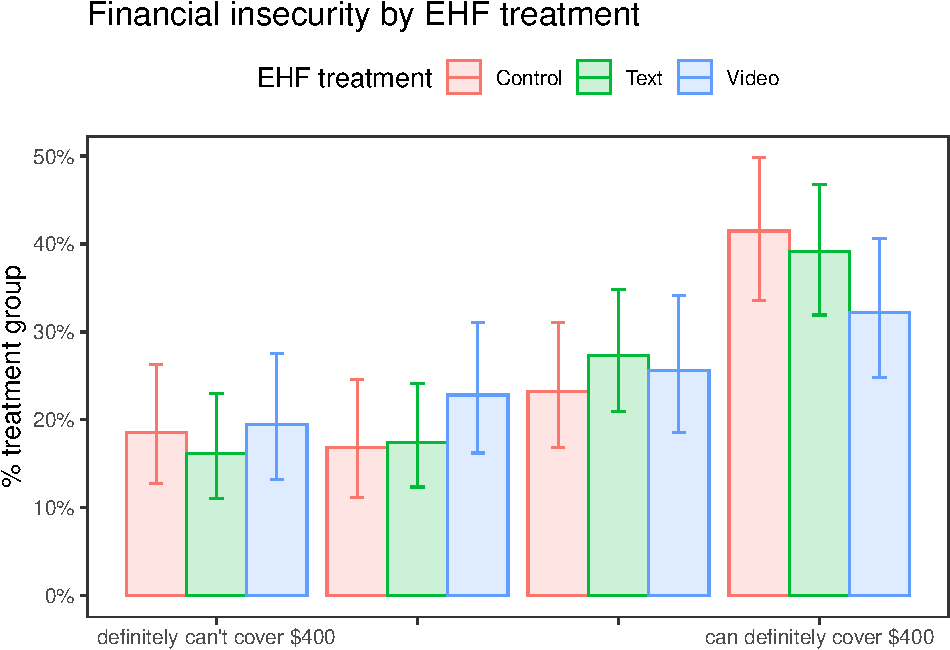
\includegraphics{EHF_Spring2025_files/figure-latex/fig-finsec-1.pdf}
\caption{\label{fig:fig-finsec}Subjective financial security (weighted)}
\end{figure}

Three findings emerge. First, just under 40\% of respondents expressed concern about their ability to meet this financial challenge, in line with recent estimates in the Survey of Household Economics and Decision-making (\citeproc{ref-SHED2022}{Board of Governors of the Federal Reserve System 2023}). Second, to the extent the EHF treatment had any effects at all, it is concentrated in the video treatment and the direction is contrary to expectations. Respondents in the video treatment felt \emph{less} financially secure than those in the control or text treatment arms. Third, none of these treatment effects were distinguishable from 0 at conventional thresholds for inference.

Table \ref{tab:tab-finsec} presents regression results that mirror the graphical displays. In particular, I find no evidence of any treatment effects, regardless of pre-exposure status. I do, however, find that respondents who reported awareness of the program prior to the experiment were also more sanguine about their financial security, even after conditioning on tenure at the Home Depot. On average their self report is higher than the unaware by about 0.5 standard deviations or half the average distance between outcome categories. Although this higher level of reported security among the pre-exposed is consistent with the EHF's improving financial security, the lack of any detectable treatment effects among the un-exposed militates against this interpretation, as we will see below. In Appendix \ref{app-bills}, I also examine an alternative outcome: the self-reported difficulty in covering monthly bills. Analysis of this secondary outcome are consistent with the those in Figure \ref{fig:fig-finsec}: presenting Home Depot employees with information about their employer's EHF, even as heavy-handed corporate propaganda, has no effect on their feelings of financial well-being.

\begin{table}
\centering
\caption{\label{tab:tab-finsec}Ability to meet emergency expense; OLS estimates \label{tab:tab-finsec}}
\centering
\begin{threeparttable}
\begin{tabular}[t]{lccc}
\toprule
  & Base & Pre-exposure & Covariates\\
\midrule
Text treatment & \num{-0.007} & \num{0.030} & \num{0.043}\\
 & (\num{0.039}) & (\num{0.066}) & (\num{0.064})\\
Video treatment & \num{-0.056} & \num{-0.051} & \num{-0.067}\\
 & (\num{0.042}) & (\num{0.072}) & (\num{0.069})\\
Pre-exposed &  & \num{0.210}** & \num{0.203}**\\
 &  & (\num{0.060}) & (\num{0.058})\\
Text x pre-exposed &  & \num{-0.066} & \num{-0.076}\\
 &  & (\num{0.080}) & (\num{0.079})\\
Video x pre-exposed &  & \num{-0.013} & \num{0.031}\\
 &  & (\num{0.087}) & (\num{0.084})\\
\midrule
$N$ & \num{515} & \num{515} & \num{509}\\
Covariates? & No & No & Yes\\
$R^2$ & \num{0.00} & \num{0.06} & \num{0.15}\\
$F$ & \num{1.05} & \num{6.33} & \num{8.14}\\
\bottomrule
\end{tabular}
\begin{tablenotes}
\item * p $<$ 0.05, ** p $<$ 0.01 Robust standard errors in parentheses. Covariates include age, gender race, job tenure, hourly status, full time status, college degree, and main job.
\end{tablenotes}
\end{threeparttable}
\end{table}

\subsection{Attitudes towards co-workers and employer}\label{attitudes-towards-co-workers-and-employer}

EHFs may not improve subjective financial security, but they may improve worker attachment to one another and the employer. We asked respondents to report how loyal they felt toward their co-workers and their employer, with responses in four categories ranging from ``none at all'' to ``a lot''. We also asked respondents how willing they would be to recommend their employer to a friend as a place to work. Figures \ref{fig:fig-loyalty} displays the distribution of responses by treatment groups across all three questions.

\begin{figure}
\centering
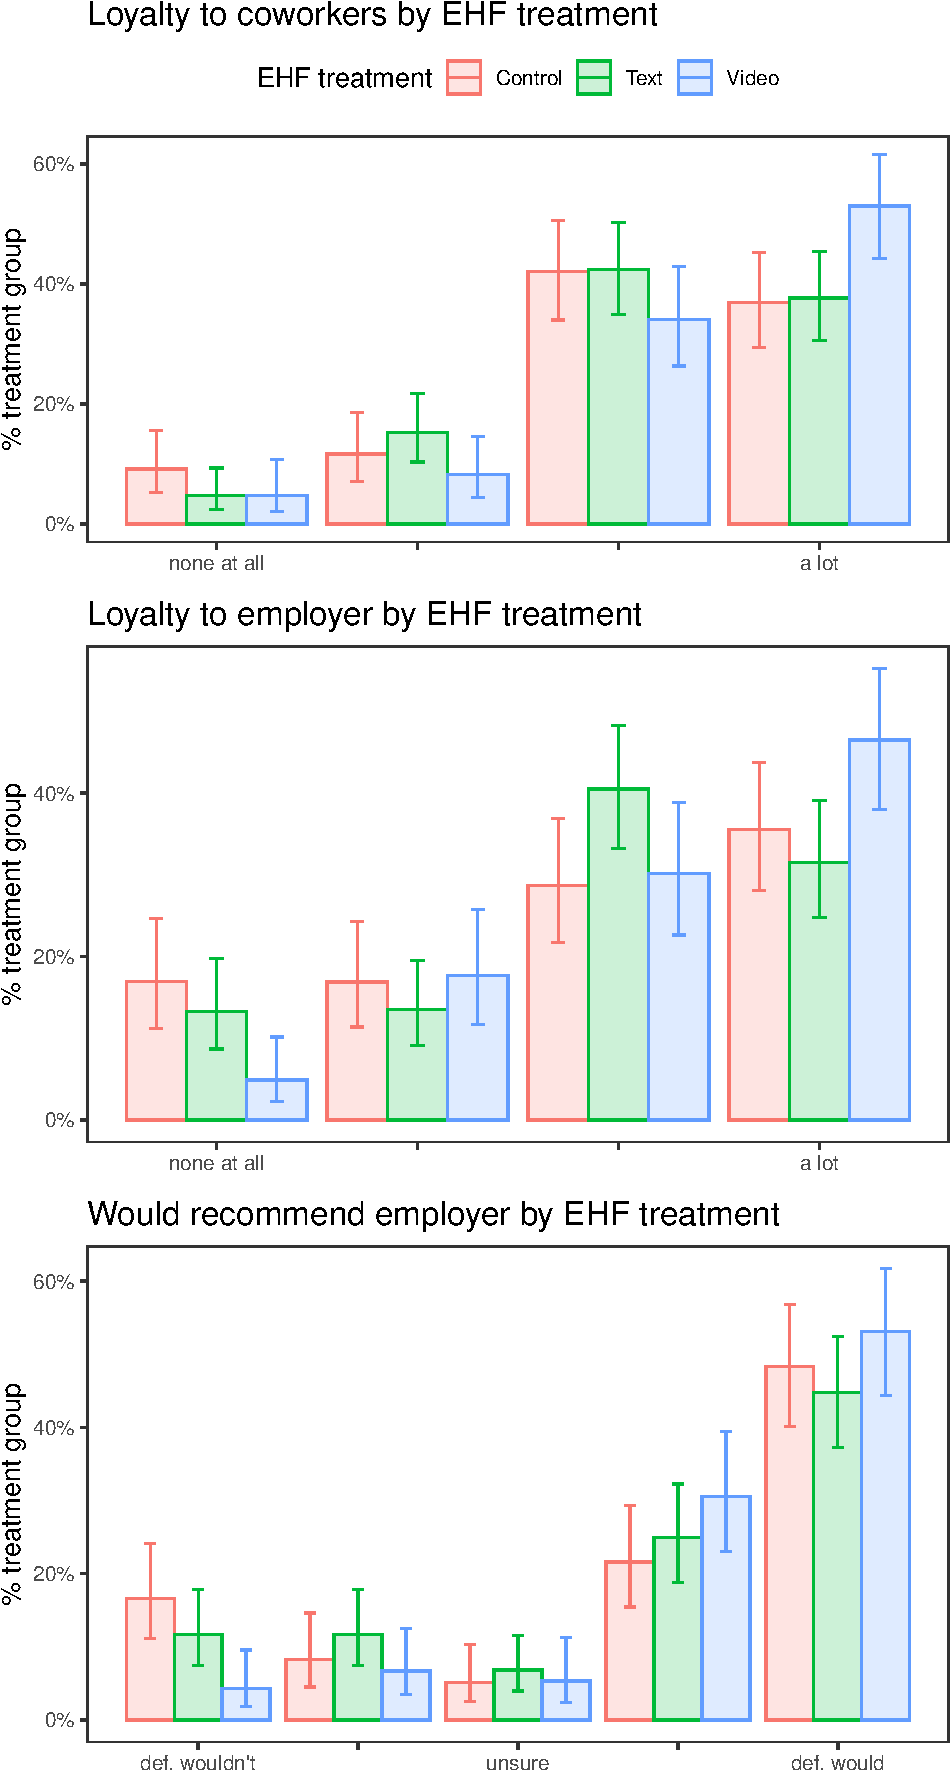
\includegraphics{EHF_Spring2025_files/figure-latex/fig-loyalty-1.pdf}
\caption{\label{fig:fig-loyalty}Attachment to co-workers and employer (weighted)}
\end{figure}

Across the various measurement options, we consistently find that respondents are reasonably positive on their co-workers and their employer. In two thirds of the treatment-outcome combinations, the most extreme positive answer was the modal response. We also see that respondents were, on average, more positively disposed to co-workers than the employer.

On average, the text treatment had no effect but the video treatment has a noticeable positive impact on all three outcome variables. Respondents exposed to the video describing the EHF in the context of a specific worker became noticeably more positive about their coworkers and their employer, although the pattern differed somewhat across outcome items. For the co-worker loyalty item, the video treatment caused a notable increase in the top category and declines in all others whereas in the two questions looking at the employer, the video treatment caused a large and significant decrease in responses in the bottom category with more modest (relative to estimation uncertainty) increases in positive responses. Looking at net promoter score (\% promoters - \% detractors) for the employer recommendation question, we see that the video treatment caused an increase from 45 under control to 73; the difference between control and the text treatment was negligible.

To put more precision on these estimates and account for covariates, we report OLS regressions for each of the loyalty/attachment measures.\footnote{Results are robust to ordered logit specifications; see Appendix \ref{app-ol}.} We report results in Table \ref{tab:tab-loyalty-models}.

\begin{table}
\centering
\caption{\label{tab:tab-loyalty-models}Coworker and employer attachment, OLS regression \label{tab:tab-loyalty-models}}
\centering
\begin{threeparttable}
\begin{tabular}[t]{lccc}
\toprule
  & Base & Pre-exposure & Covariates\\
\midrule
\addlinespace[0.5em]
\multicolumn{4}{l}{\textit{Outcome: co-worker loyalty}}\\
\midrule \hspace{1em}Text treatment & 0.002 & 0.103 & 0.097\\
\hspace{1em} & (0.031) & (0.054) & (0.055)\\
\hspace{1em}Video treatment & 0.085** & 0.158** & 0.148*\\
\hspace{1em} & (0.032) & (0.059) & (0.058)\\
\hspace{1em}Pre-exposed &  & 0.227** & 0.215**\\
\hspace{1em} &  & (0.049) & (0.049)\\
\hspace{1em}Text x pre-exposed &  & -0.172** & -0.173**\\
\hspace{1em} &  & (0.065) & (0.067)\\
\hspace{1em}Video x pre-exposed &  & -0.125 & -0.116\\
\hspace{1em} &  & (0.068) & (0.067)\\
\hspace{1em}$N$ & 514 & 514 & 508\\
\hspace{1em}$R^2$ & 0.02 & 0.08 & 0.11\\
\hspace{1em}$F$ & 5.14 & 8.05 & 4.89\\
\addlinespace[0.5em]
\multicolumn{4}{l}{\textit{Outcome: employer loyalty}}\\
\midrule \hspace{1em}Text treatment & -0.002 & 0.020 & \vphantom{1} 0.008\\
\hspace{1em} & (0.037) & (0.063) & \vphantom{1} (0.061)\\
\hspace{1em}Video treatment & 0.089* & 0.120 & \vphantom{1} 0.094\\
\hspace{1em} & (0.037) & (0.065) & \vphantom{1} (0.062)\\
\hspace{1em}Pre-exposed &  & 0.186** & \vphantom{1} 0.164**\\
\hspace{1em} &  & (0.059) & \vphantom{1} (0.057)\\
\hspace{1em}Text x pre-exposed &  & -0.038 & \vphantom{1} -0.026\\
\hspace{1em} &  & (0.076) & \vphantom{1} (0.075)\\
\hspace{1em}Video x pre-exposed &  & -0.053 & \vphantom{1} -0.028\\
\hspace{1em} &  & (0.078) & \vphantom{1} (0.076)\\
\hspace{1em}$N$ & 508 & 508 & \vphantom{1} 502\\
\hspace{1em}$R^2$ & 0.02 & 0.07 & \vphantom{1} 0.16\\
\hspace{1em}$F$ & 4.43 & 7.14 & \vphantom{1} 7.83\\
\addlinespace[0.5em]
\multicolumn{4}{l}{\textit{Outcome: recommend employer}}\\
\midrule \hspace{1em}Text treatment & -0.002 & 0.020 & 0.008\\
\hspace{1em} & (0.037) & (0.063) & (0.061)\\
\hspace{1em}Video treatment & 0.089* & 0.120 & 0.094\\
\hspace{1em} & (0.037) & (0.065) & (0.062)\\
\hspace{1em}Pre-exposed &  & 0.186** & 0.164**\\
\hspace{1em} &  & (0.059) & (0.057)\\
\hspace{1em}Text x pre-exposed &  & -0.038 & -0.026\\
\hspace{1em} &  & (0.076) & (0.075)\\
\hspace{1em}Video x pre-exposed &  & -0.053 & -0.028\\
\hspace{1em} &  & (0.078) & (0.076)\\
\hspace{1em}$N$ & 508 & 508 & 502\\
\hspace{1em}$R^2$ & 0.02 & 0.07 & 0.16\\
\hspace{1em}$F$ & 4.43 & 7.14 & 7.83\\
\bottomrule
\end{tabular}
\begin{tablenotes}
\item * p $<$ 0.05, ** p $<$ 0.01 Robust standard errors in parentheses. Covariates include age, gender race, job tenure, hourly status, full time status, college degree, and main job.
\end{tablenotes}
\end{threeparttable}
\end{table}

Across models and specifications we recover a positive and precisely estimated treatment effect for the video condition. The coefficient for the text treatment is consistently positive but far smaller and indistinguishable from 0. In terms of magnitude, the video treatment effect averages about 0.1 standard deviations on the relevant scale. We also uncover important heterogeneity by pre-exposure status. As before, those pre-exposed to the EHF were significantly more positive towards both co-workers and the employer than the un-exposed by about 0.5 standard deviations. But, unlike for financial security, we see significant treatment effects that vary by pre-exposure status. Across all three outcomes, the positive treatment effects were concentrated almost entirely among those unaware of the EHF before the survey, with near-zero treatment effects among those already exposed to this information.

To see the heterogeneous effects more clearly, Figure \ref{fig:fig-effattach} displays average predicted outcomes by treatment and pre-exposure status for the co-worker and employer loyalty outcomes (both measured on the same scale). Looking at co-worker loyalty on the left, we see that, among the unaware, the text treatment produced a positive and marginally significant treatment effect and the video treatment elicited a significant effect on the order of 0.6 standard deviations. Among the pre-exposed the treatment effects vanish. Looking at the employer loyalty outcome, we see somewhat weaker effects. Among the unexposed, the text treatment produces no detectable effect while the video treatment elicits a significant effect of about one third of a standard deviation. Among the exposed, we also uncover a positive though smaller effect for the video treatment only. Findings here suggest that simply informing workers by providing dry, technical summaries of an EHF has little impact on their attachment to employers or co-workers. More intensive ``propaganda'', on the other hand, shows a marked increase in attachment, although effects are largely concentrated among the unaware and stronger for coworkers than for the employer. Whether these effects are durable or fade rapidly is unknown.

\begin{figure}
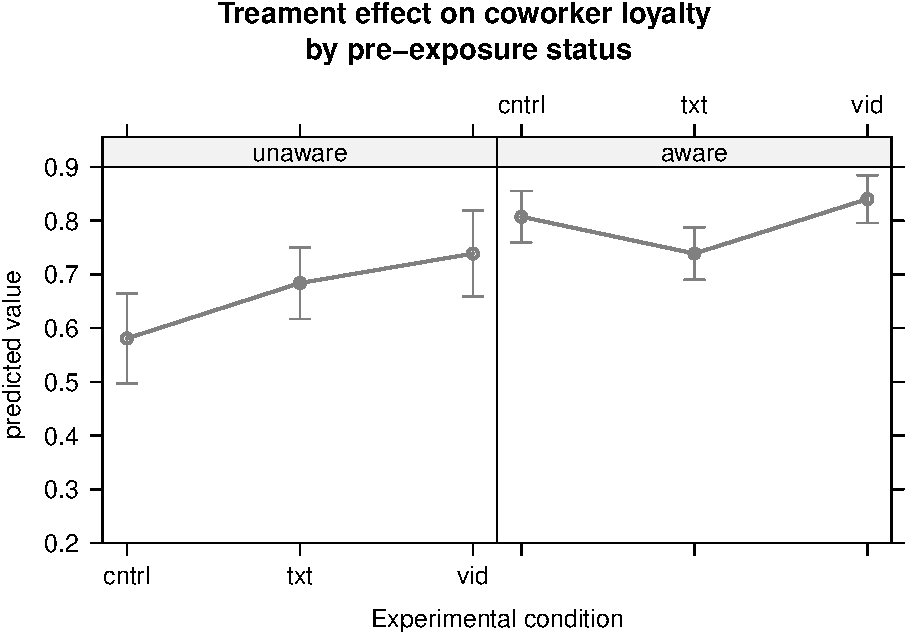
\includegraphics[width=0.5\linewidth]{EHF_Spring2025_files/figure-latex/fig-effattach-1} 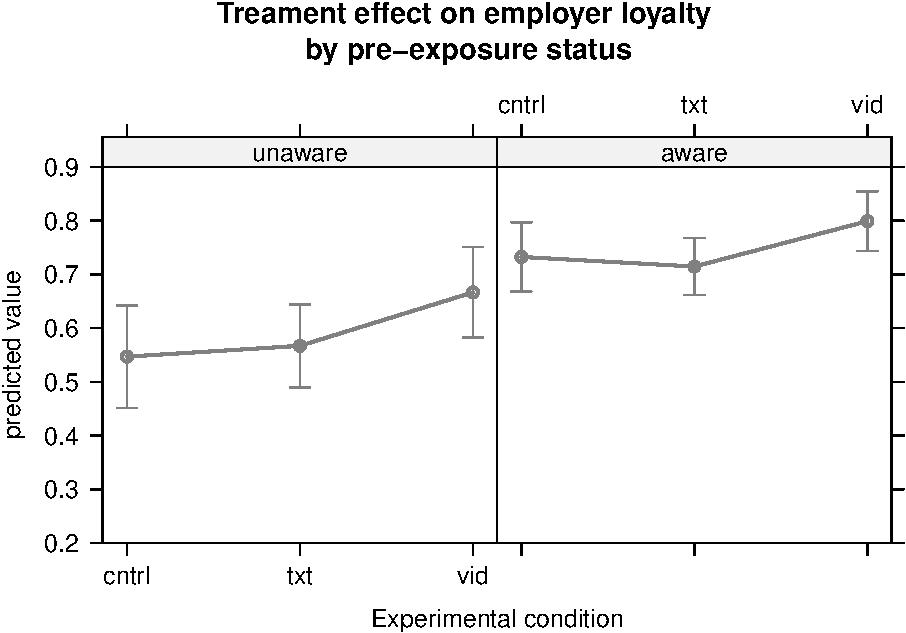
\includegraphics[width=0.5\linewidth]{EHF_Spring2025_files/figure-latex/fig-effattach-2} \caption{Interpreting treatment effects on attachment by pre-exposure status}\label{fig:fig-effattach}
\end{figure}

\subsubsection{Attitudes toward unionization}\label{attitudes-toward-unionization}

These final two sections discuss experimental effects on support for unionization and government-provided social insurance. For unionization, respondents answered the standard union vote question: ``If an election were held today to decide whether employees like you should be represented by a union at The Home Depot, would you vote for the union or against the union?'' Respondents could answer \{yes, no, not sure\}. In examining social insurance, I take a question battery from the GSS that asks the extent to which the respondent thinks the government has a responsibility to provide for different constituencies. Here I examine responses for ``the unemployed'' (4-category response ranging from ``none at all'' to ``a lot''). The distribution of responses to both questions by EHF treatment is displayed in Figure \ref{fig:fig-uvui}.

\begin{figure}
\centering
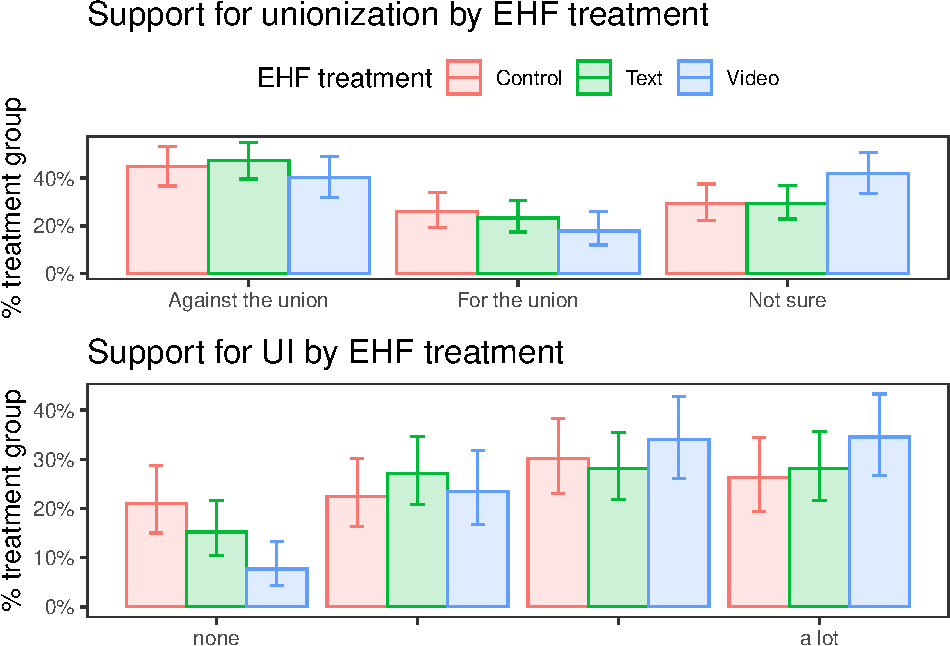
\includegraphics{EHF_Spring2025_files/figure-latex/fig-uvui-1.pdf}
\caption{\label{fig:fig-uvui}Support for unions and unemployment insurance (weighted)}
\end{figure}

We see that workers in this sample are generally skeptical of unions, with 25\% of control respondents reporting a willingness to vote for a union and 48\% voting against (the remainder answered ``not sure''). This level of union support is substantially lower than recent estimates among front line retail workers.\footnote{In Study 1, we found that 44\% would vote for a union and 20\% against. Ahlquist, Grumbach, and Thai (\citeproc{ref-AGT_youngworkers}{2023}); Workers Empowerment Research Network (\citeproc{ref-WERNsurvey2023}{2023}) find that 36\% of retail workers would vote for the union and 26\% would vote against.} There are, however, a substantial portion of undecided workers, the modal response among the video treatment group.

Turning to treatment effects, we see some surprising results. First, echoing findings for the attachment questions, we find no evidence that the text treatment has any average effect at all for either outcome. Second, we find that the video treatment again moves respondents' opinions. On average, the video treatment makes respondents more \emph{uncertain} about their support for unionization. The fact that respondents chose to answer the question (as opposed to skipping it) suggests that findings here represent actual increased uncertainty, as opposed to respondent disinterest.

Given the importance of all three outcome categories, I report multinomial logit results in table \ref{tab:tab-uv}. In the base model we see that video treatment, on average, produces an increase in the ``not sure'' responses, echoing Figure \ref{fig:fig-uvui}. But accounting for pre-exposure status in a regression framework is particularly illuminating here. Once we condition on pre-exposure, we see that those aware of the EHF prior to the experiment were significantly less supportive of unions than the unexposed. Among the unexposed, we see that both the text and video treatments reduce support for unionization, although the video treatment effect is the only one that crosses conventional significance thresholds.

\begin{table}
\centering
\begin{talltblr}[         %% tabularray outer open
caption={Multinomial logistic regression of union support \label{tab:tab-uv}},
note{}={* p \num{< 0.05}, ** p \num{< 0.01}},
note{ }={Reference category is 'For the union'. Covariates include age, gender race, job tenure, full time status, college degree, and main job.  Hourly worker indicator was excluded due to perfect separation.},
]                     %% tabularray outer close
{                     %% tabularray inner open
colspec={Q[]Q[]Q[]Q[]Q[]Q[]Q[]Q[]},
cell{2}{3}={}{halign=c,},
cell{2}{4}={}{halign=c,},
cell{2}{5}={}{halign=c,},
cell{2}{6}={}{halign=c,},
cell{2}{7}={}{halign=c,},
cell{2}{8}={}{halign=c,},
cell{3}{3}={}{halign=c,},
cell{3}{4}={}{halign=c,},
cell{3}{5}={}{halign=c,},
cell{3}{6}={}{halign=c,},
cell{3}{7}={}{halign=c,},
cell{3}{8}={}{halign=c,},
cell{4}{3}={}{halign=c,},
cell{4}{4}={}{halign=c,},
cell{4}{5}={}{halign=c,},
cell{4}{6}={}{halign=c,},
cell{4}{7}={}{halign=c,},
cell{4}{8}={}{halign=c,},
cell{5}{3}={}{halign=c,},
cell{5}{4}={}{halign=c,},
cell{5}{5}={}{halign=c,},
cell{5}{6}={}{halign=c,},
cell{5}{7}={}{halign=c,},
cell{5}{8}={}{halign=c,},
cell{6}{3}={}{halign=c,},
cell{6}{4}={}{halign=c,},
cell{6}{5}={}{halign=c,},
cell{6}{6}={}{halign=c,},
cell{6}{7}={}{halign=c,},
cell{6}{8}={}{halign=c,},
cell{7}{3}={}{halign=c,},
cell{7}{4}={}{halign=c,},
cell{7}{5}={}{halign=c,},
cell{7}{6}={}{halign=c,},
cell{7}{7}={}{halign=c,},
cell{7}{8}={}{halign=c,},
cell{8}{3}={}{halign=c,},
cell{8}{4}={}{halign=c,},
cell{8}{5}={}{halign=c,},
cell{8}{6}={}{halign=c,},
cell{8}{7}={}{halign=c,},
cell{8}{8}={}{halign=c,},
cell{9}{3}={}{halign=c,},
cell{9}{4}={}{halign=c,},
cell{9}{5}={}{halign=c,},
cell{9}{6}={}{halign=c,},
cell{9}{7}={}{halign=c,},
cell{9}{8}={}{halign=c,},
cell{10}{3}={}{halign=c,},
cell{10}{4}={}{halign=c,},
cell{10}{5}={}{halign=c,},
cell{10}{6}={}{halign=c,},
cell{10}{7}={}{halign=c,},
cell{10}{8}={}{halign=c,},
cell{11}{3}={}{halign=c,},
cell{11}{4}={}{halign=c,},
cell{11}{5}={}{halign=c,},
cell{11}{6}={}{halign=c,},
cell{11}{7}={}{halign=c,},
cell{11}{8}={}{halign=c,},
cell{12}{3}={}{halign=c,},
cell{12}{4}={}{halign=c,},
cell{12}{5}={}{halign=c,},
cell{12}{6}={}{halign=c,},
cell{12}{7}={}{halign=c,},
cell{12}{8}={}{halign=c,},
cell{13}{3}={}{halign=c,},
cell{13}{4}={}{halign=c,},
cell{13}{5}={}{halign=c,},
cell{13}{6}={}{halign=c,},
cell{13}{7}={}{halign=c,},
cell{13}{8}={}{halign=c,},
cell{14}{3}={}{halign=c,},
cell{14}{4}={}{halign=c,},
cell{14}{5}={}{halign=c,},
cell{14}{6}={}{halign=c,},
cell{14}{7}={}{halign=c,},
cell{14}{8}={}{halign=c,},
cell{1}{4}={}{halign=c, halign=c,},
cell{1}{6}={}{halign=c, halign=c,},
cell{1}{8}={}{halign=c, halign=c,},
cell{2}{1}={}{halign=l,},
cell{2}{2}={}{halign=l,},
cell{3}{1}={}{halign=l,},
cell{3}{2}={}{halign=l,},
cell{4}{1}={}{halign=l,},
cell{4}{2}={}{halign=l,},
cell{5}{1}={}{halign=l,},
cell{5}{2}={}{halign=l,},
cell{6}{1}={}{halign=l,},
cell{6}{2}={}{halign=l,},
cell{7}{1}={}{halign=l,},
cell{7}{2}={}{halign=l,},
cell{8}{1}={}{halign=l,},
cell{8}{2}={}{halign=l,},
cell{9}{1}={}{halign=l,},
cell{9}{2}={}{halign=l,},
cell{10}{1}={}{halign=l,},
cell{10}{2}={}{halign=l,},
cell{11}{1}={}{halign=l,},
cell{11}{2}={}{halign=l,},
cell{12}{1}={}{halign=l,},
cell{12}{2}={}{halign=l,},
cell{13}{1}={}{halign=l,},
cell{13}{2}={}{halign=l,},
cell{14}{1}={}{halign=l,},
cell{14}{2}={}{halign=l,},
cell{1}{1}={}{halign=l, halign=c,},
cell{1}{2}={}{halign=l, halign=c,},
cell{1}{3}={c=2,}{halign=c, halign=c, halign=c,},
cell{1}{5}={c=2,}{halign=c, halign=c, halign=c,},
cell{1}{7}={c=2,}{halign=c, halign=c, halign=c,},
hline{13}={1,2,3,4,5,6,7,8}{solid, black, 0.05em},
}                     %% tabularray inner close
\toprule
&  & Base &  & Pre-exposure &  & Covariates &  \\ \cmidrule[lr]{3-4}\cmidrule[lr]{5-6}\cmidrule[lr]{7-8}
& response & Est. & S.E. & Est. & S.E. & Est. & S.E. \\ \midrule %% TinyTableHeader
Text treatment & Against the union & \num{0.191} & \num{0.266} & \num{0.605} & \num{0.409} & \num{0.458} & \num{0.428} \\
& Not sure & \num{0.153} & \num{0.297} & \num{0.642} & \num{0.432} & \num{0.662} & \num{0.443} \\
Video treatment & Against the union & \num{0.368} & \num{0.307} & \num{1.105}* & \num{0.484} & \num{1.018}* & \num{0.499} \\
& Not sure & \num{0.872}** & \num{0.323} & \num{1.389}** & \num{0.495} & \num{1.312}** & \num{0.505} \\
Pre-exposed & Against the union &  &  & \num{1.318}** & \num{0.405} & \num{1.244}** & \num{0.424} \\
& Not sure &  &  & \num{0.852} & \num{0.442} & \num{0.941}* & \num{0.456} \\
Text x pre-exposed & Against the union &  &  & \num{-0.813} & \num{0.552} & \num{-0.685} & \num{0.573} \\
& Not sure &  &  & \num{-0.976} & \num{0.602} & \num{-0.940} & \num{0.614} \\
Video x pre-exposed & Against the union &  &  & \num{-1.334}* & \num{0.637} & \num{-1.247} & \num{0.656} \\
& Not sure &  &  & \num{-1.010} & \num{0.662} & \num{-1.010} & \num{0.677} \\
$N$ &  & \num{514} &  & \num{514} &  & \num{508} &  \\
AIC &  & \num{1077} &  & \num{1074} &  & \num{1044} &  \\
\bottomrule
\end{talltblr}
\end{table}

Figure \ref{fig:fig-uveff} provides a graphical interpretation of treatment effect by pre-exposure status. The left column displays the predicted outcomes by treatment status for those who were not aware of the EHF before the survey. This right column displays the same quantities for those already aware of the EHF. On the left, we clearly see that the treatments, especially the video version, reduce support for unionization. Predicted union support among the unaware respondents exposed to the video treatment is effectively identical to that among the aware. But rather than increasing opposition, the video treatment makes the unaware respondents more unsure. In the right hand column we see that the video treatment actually reduces opposition to unionization among those who were already aware of the EHF. But, again, this effect comes from an increase the ``not sure'' responses. Overall, we see evidence consistent with the idea that EHFs reduce support for unionization, largely by increasing uncertainty or apathy as opposed to encouraging opposition.

\begin{figure}
\centering
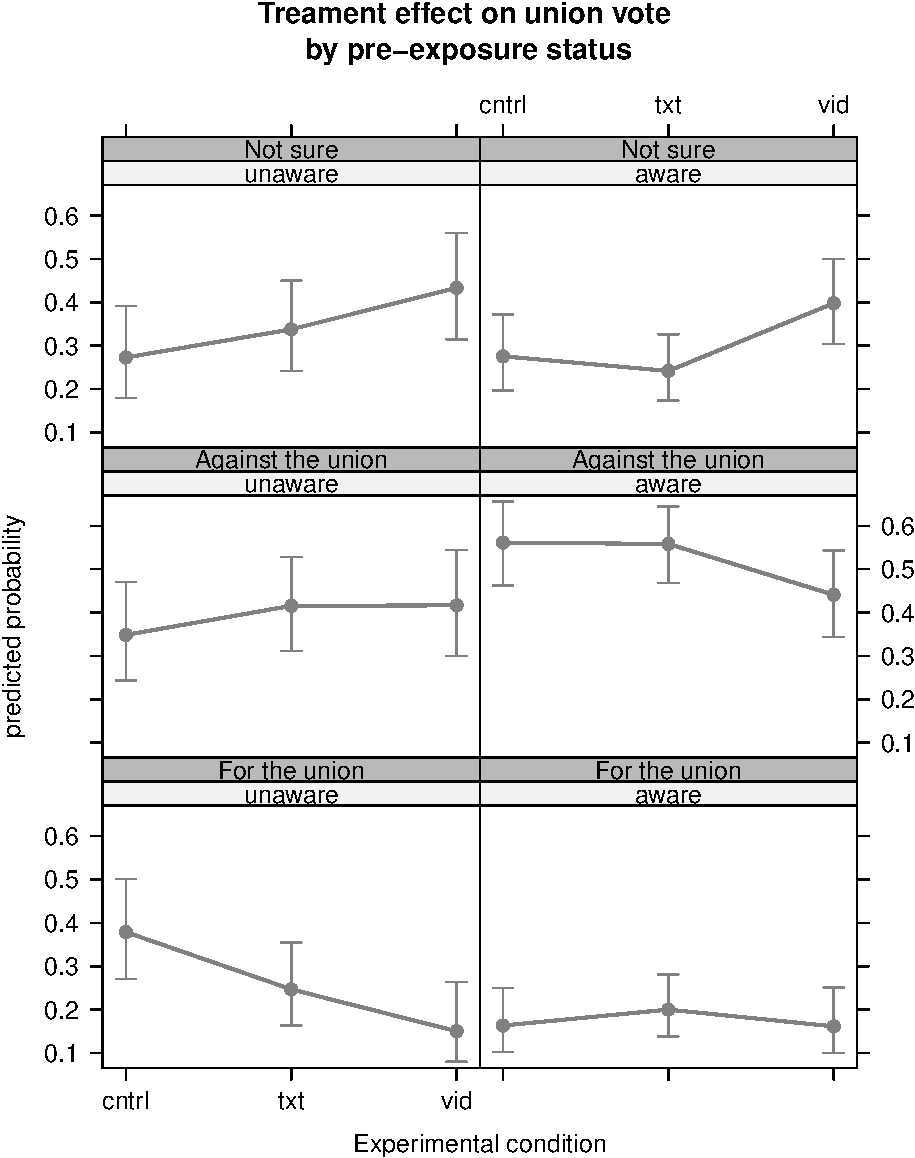
\includegraphics{EHF_Spring2025_files/figure-latex/fig-uveff-1.pdf}
\caption{\label{fig:fig-uveff}Interpreting treatment effects from union vote models}
\end{figure}

\subsubsection{Attitudes toward government social insurance}\label{attitudes-toward-government-social-insurance}

Compared to unionization, workers in this sample are far more supportive of unemployment insurance, with a solid majority viewing the government as at least somewhat responsible for the welfare of the unemployed. We see that the video treatment substantially reduces the proportion of responses in the ``none'' category in favor of the two positive categories. The EHF video treatment made respondents more rather than less supportive of government-provided social insurance, contrary to expectations. The text treatment, on the other hand, does not appear to have any detectable treatment effect on average.

\begin{table}
\centering
\begin{talltblr}[         %% tabularray outer open
caption={Support for Unemployment Insurance \label{tab:tab-ui}},
note{}={* p \num{< 0.05}, ** p \num{< 0.01}},
note{ }={Robust standard errors in parentheses.
 Covariates include age, gender race, job tenure, hourly status, full time status, college degree, and main job.},
]                     %% tabularray outer close
{                     %% tabularray inner open
colspec={Q[]Q[]Q[]Q[]},
column{2,3,4}={}{halign=c,},
column{1}={}{halign=l,},
hline{12}={1,2,3,4}{solid, black, 0.05em},
}                     %% tabularray inner close
\toprule
& Base & Pre-exposure & Covariates \\ \midrule %% TinyTableHeader
Text treatment & \num{0.032} & \num{-0.053} & \num{-0.055} \\
& (\num{0.037}) & (\num{0.063}) & (\num{0.063}) \\
Video treatment & \num{0.108}** & \num{0.031} & \num{0.033} \\
& (\num{0.038}) & (\num{0.061}) & (\num{0.059}) \\
Pre-exposed &  & \num{-0.105} & \num{-0.102} \\
&  & (\num{0.057}) & (\num{0.056}) \\
Text x pre-exposed &  & \num{0.141} & \num{0.149} \\
&  & (\num{0.078}) & (\num{0.078}) \\
Video x pre-exposed &  & \num{0.127} & \num{0.116} \\
&  & (\num{0.078}) & (\num{0.077}) \\
$N$ & \num{511} & \num{511} & \num{506} \\
Covariates? & No & No & Yes \\
$R^2$ & \num{0.02} & \num{0.02} & \num{0.09} \\
$F$ & \num{4.29} & \num{2.54} & \num{3.97} \\
\bottomrule
\end{talltblr}
\end{table}

Table \ref{tab:tab-ui} displays regression estimates for UI support. Results here confirm a positive average treatment effect for the video treatment of about 0.31 standard deviations. In contrast to all of the outcomes studied above, we see no large or statistically discernible difference between the pre-exposed and unaware in average support for UI. We also see no treatment effects among the unaware, although there are treatment effects among the \emph{pre-exposed}, especially for the video treatment.

To interpret this more easily, Figure \ref{fig:fig-uieff} displays treatment effects by respondent pre-exposure to the EHF. In the case of UI, we see that treatment effects are entirely concentrated among those \emph{already} aware of the Home Depot's EHF. Contrary to expectations, both the text and video treatments \emph{increase} support for UI, although only the latter is a significant effect by conventional standards. This finding deserves more exploration, but it consistent with author interviews with EHF professionals in which they indicate that EHFs are meant to supplement or provide a bridge to public benefits, rather than supplant them.

\begin{figure}
\centering
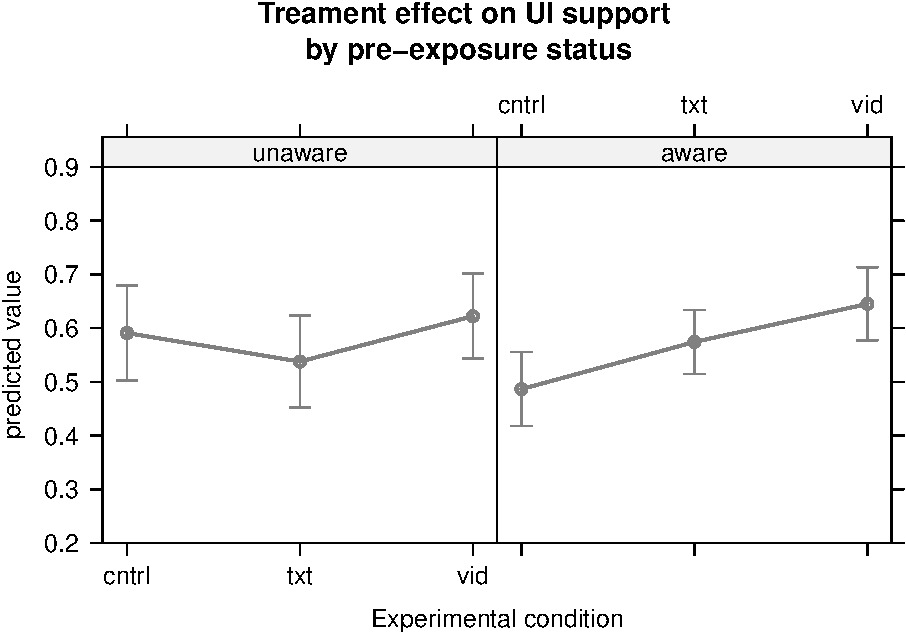
\includegraphics{EHF_Spring2025_files/figure-latex/fig-uieff-1.pdf}
\caption{\label{fig:fig-uieff}Interpreting treatment effects from UI models}
\end{figure}

Is unemployment insurance the appropriate policy to link with the EHF? After all, the EHF is designed to provide benefits while having a job with this employer whereas UI is designed to help when a job is lost.\footnote{The pre-exposed may better appreciate this distinction, which may help explain the unexpected findings.} There are two pieces of evidence that UI is a reasonable policy domain to link with EHF benefits. First, although EHF benefits are not available to someone who loses her job with an employer, benefits are often available when a worker's immediate family member loses a job. Second, the UI question was asked as part of a battery of questions asking about UI was well as two other policy areas: pensions for the elderly and the provision of childcare for working parents. These two questions can constitute ``placebos'' since EHFs have no connection with either policy area. Parameter estimates from regressing support for these alternative policy areas on the EHF treatments and EHF awareness appear in Appendix Table \ref{tab:tab-placebo}. I find no evidence for any relationship between the EHF treatments and support for government involvement in either old age pensions or childcare, regardless of whether the respondent was aware of the EHF going into the survey.

\section{Study 3}\label{study-3}

\subsection{Case selection and survey}\label{case-selection-and-survey}

Do the results from Study 2 replicate at other large US retailers? Or is the Home Depot something of an outlier? Based on the results from Study 2, we conducted a third study, this time focusing on another publicly traded ``big box'' retailer: Walmart. Walmart and Home Depot compete to some degree, including for workers. Walmart has seen union activism in some locations. Walmart is the largest retailer (and private sector employer) in the United States, over three times as large the Home Depot in employee headcount, making the social media recruitment strategy feasible. With its size and ubiquity, Walmart job benefits, programs, and procedures have an impact on the retail industry as a whole.

As with the HF, Walmart's ACNT Together Fund is over 20 years old and managed in-house. The EHF is available to both full- and part-time workers who have been at Walmart for at least one year. But the ACNT is substantially less generous than the HF and operates on a smaller scale, notwithstanding Walmart's considerably larger presence. And Walmart appears to engage in less internal promotion around its EHF.\footnote{Interestingly, Walmart matches employee donations to the Walmart political action committee 2:1 with corporate donations to the Together Fund. This practice that was challenged but found legal by the Federal Election Commission in 2015. In our sample, less than 1\% of respondents reported making a contribution to the Walmart PAC.} The ACNT Together Fund has a minimal social media presence. EHF practitioners regularly pointed to the Home Depot as exemplary in their EHF promotion activities and incentives as well as integration with the broader corporate culture, including both worker support programs and corporate philanthropy while also pointing out that Walmart is less aggressive in all these areas.

In fielding a survey of Walmart workers, I followed the same social media recruitment strategy as with the Home Depot. Survey completers were offered the opportunity to enter a raffle for a \$400 gift card. The survey was in the field from October 23 to December 4, 2024 and produced 980 complete responses that passed screening and attention checks. We produce raking weights for the Walmart sample in a manner analogous to the Home Depot and employ them below in the same way. Survey descriptive statistics by treatment status appear in Appendix XX.

The surveys in Studies 2 and 3 were very similar in question wording and ordering, but there were four main extensions in Study 3: we asked about quit intentions and job amenities; we included a behavioral measure of donation to the EHF (clicking on a link to a donation page); we expanded the EHF survey experiment; and we sent a follow-up survey one week after survey completion to respondents who opted in to the incentive raffle.\footnote{Respondents were sent emails to invite them into the follow-up survey, offering them a second entry into the raffle for follow-up completion. Respondents were contacted a maximum of three times. We received valid followup responses from 157 or 16\% of those completing the main survey.}

\subsection{ACNT awareness and engagement}\label{acnt-awareness-and-engagement}

As expected, EHF awareness and engagement is substantially lower among the Walmart sample than among the Home Depot workers. We find that 38\% (se = 2\%) were aware of the ACNT. Of those who both knew about the ACNT \emph{and} experienced a qualifying event, 17\% applied for a grant. 17\% (se = 2\%) claim to know a grant recipient and 11\% (se = 1\%) claim to have donated.

Table \ref{tab:tab-awareness-model-wmt} presents regression results for the correlates of awareness and engagement. Consistent with the Home Depot results, job tenure is a consistently important predictor of awareness and men are less engaged with the ACNT. I also note that job tenure in the Walmart is considerably shorter than for the Home depot.\footnote{The median Walmart respondent had been employed at Walmart between 2 and 3 years whereas the median Home Depot respondent had been with the Home Depot for over 3 years.}

\begin{table}
\centering
\caption{\label{tab:ACNT-aware-calcs}Weighted logistic regression of EHF awareness and engagement \label{tab:tab-awareness-model-wmt}}
\centering
\begin{threeparttable}
\begin{tabular}[t]{lccccc}
\toprule
  & awareness & know recipient & applied & received & donated\\
\midrule
age & \num{-0.009} & \num{-0.010} & \num{-0.011} & \num{0.001} & \num{0.001}\\
 & (\num{0.006}) & (\num{0.009}) & (\num{0.008}) & (\num{0.003}) & (\num{0.010})\\
male & \num{-0.328}* & \num{-0.754}** & \num{-0.754}* & \num{-0.320}** & \num{-0.720}*\\
 & (\num{0.166}) & (\num{0.273}) & (\num{0.318}) & (\num{0.091}) & (\num{0.345})\\
tenure & \num{0.020}** & \num{0.037}** & \num{0.029}** & \num{-0.000} & \num{0.023}*\\
 & (\num{0.006}) & (\num{0.009}) & (\num{0.010}) & (\num{0.003}) & (\num{0.011})\\
nonwhite & \num{0.206} & \num{0.509} & \num{0.782}** & \num{-0.012} & \num{0.797}**\\
 & (\num{0.183}) & (\num{0.266}) & (\num{0.273}) & (\num{0.100}) & (\num{0.304})\\
full time & \num{0.758}** & \num{0.711}* & \num{-0.047} & \num{0.012} & \num{0.537}\\
 & (\num{0.209}) & (\num{0.328}) & (\num{0.318}) & (\num{0.104}) & (\num{0.416})\\
hourly & \num{-0.783}* & \num{-1.078}* & \num{2.152}* & \num{0.033} & \num{-2.718}**\\
 & (\num{0.364}) & (\num{0.528}) & (\num{1.044}) & (\num{0.218}) & (\num{0.498})\\
college & \num{-0.067} & \num{0.100} & \num{-0.111} & \num{-0.067} & \num{0.266}\\
 & (\num{0.241}) & (\num{0.388}) & (\num{0.434}) & (\num{0.134}) & (\num{0.414})\\
\midrule
$N$ & \num{980} & \num{725} & \num{725} & \num{725} & \num{725}\\
AIC & \num{1263} & \num{630} & \num{520} & \num{0} & \num{447}\\
\bottomrule
\end{tabular}
\begin{tablenotes}
\item * p $<$ 0.05, ** p $<$ 0.01 Standard errors in parentheses.
\end{tablenotes}
\end{threeparttable}
\end{table}

\subsection{Survey experiment}\label{survey-experiment}

Based on results from the Home Depot survey, I use only a video vignette treatment in the Walmart survey experiment. There were no available Walmart-produced video testimonials. To construct a video treatments as similar as possible across surveys, I used the HF video as a script and visual template to then produce an original video adapted to the Walmart context using a paid actor.\footnote{The paid actor exhibited the same gender (male) and racial (white) expression as in the HF video. The actor was also viewed as approximately the same age as the spokesperson in the HF video, according to mTurk coders. The ACNT-adapted video was 41 seconds shorter than the HF video. We achieved this by shortening or removing some interstitial and panning shots, not through any reduction in the spoken script beyond those parts that were only relevant to the Home Depot. The video included text indicating that the speaker was an actor at the beginning of the video.}

Respondents were randomly assigned with equal probability to either treatment or control. Within the control condition, respondents were randomly divided between the pure control and the placebo conditions. The pure controls saw no additional information, just as in Study 2. Respondents in the placebo condition watched a video in which the hired actor delivered a Walmart press release about the company's acquisition of Vizio.\footnote{I also pre-registered a framing study, in which I slightly vary the framing of the treatment video. Specifically, the ``card'' visible on the screen before the respondent clicks ``play'' differs, with the \emph{solidarity} framing displaying text emphasizing supporting other Walmart workers and the and the \emph{charity} framing displaying text emphasizing charitable donations to help those in need. The content of the video vignettes was otherwise identical across treatment groups. As there was no detectable difference between these framings, I do not report on this in the main text. Regression results demonstrating this for key outcomes appears in appendix {[}cite appendix{]}.} A manipulation check (see Appendix \ref{app-manip-wmt}) confirms that the video treatment did, indeed increase respondent awareness of the ACNT, as expected. There were no detectable differences between pure control and placebo groups in their (non-)effect. Thus we display results for binary treatment/control in the analysis below. Based on the findings in the Home Depot sample, we pre-registered a plan to examine whether treatment effects differ based on pre-exposure to the ACNT, measured using the same question format as in the Home Depot survey.

\subsubsection{Financial security and job attachment}\label{financial-security-and-job-attachment}

Respondents in the Walmart sample were notably more pessimistic about their financial security than in the Home Depot sample, with 65\% expressing concern about their ability to meet a \$400 emergency expense. Table \ref{tab:tab-finsec-wmt} displays OLS regression-based estimates of treatment effects. Those pre-exposed to the ACNT are more confident in their ability to meet a small financial emergency, even after conditioning on predictors of EHF awareness. But, just as with the Home Depot workers, we fail to detect any treatment effects on Walmart worker's subjective financial security.

\begin{table}
\centering
\caption{\label{tab:tab-finsec-wmt}Ability to meet emergency expense; OLS estimates \label{tab:tab-finsec-wmt}}
\centering
\begin{threeparttable}
\begin{tabular}[t]{lccc}
\toprule
  & Base & Pre-exposure & Covariates\\
\midrule
Treated & \num{-0.032} & \num{-0.025} & \num{-0.026}\\
 & (\num{0.022}) & (\num{0.028}) & (\num{0.028})\\
Pre-exposed &  & \num{0.096}** & \num{0.096}**\\
 &  & (\num{0.032}) & (\num{0.032})\\
Treated x pre-exposed &  & \num{-0.008} & \num{0.000}\\
 &  & (\num{0.046}) & (\num{0.046})\\
\midrule
Covariates? & No & No & Yes\\
$N$ & \num{980} & \num{980} & \num{980}\\
$R^2$ & \num{0.00} & \num{0.02} & \num{0.05}\\
F & \num{2.00} & \num{5.93} & \num{4.25}\\
\bottomrule
\end{tabular}
\begin{tablenotes}
\item * p $<$ 0.05, ** p $<$ 0.01 Robust standard errors in parentheses. Covariates include age, gender race, job tenure, hourly status, full time status, college degree, and main job.
\end{tablenotes}
\end{threeparttable}
\end{table}

In addition to feeling more financially precarious, Walmart respondents were less supportive of Walmart as an employer, compared to the Home Depot workers. For example, the net promoter score among the Walmart control respondents was 45\%, seven percentage points lower than at the Home Depot.

To analyze treatment effects on job attachment, I again construct a job attachment index using a principal components analysis of the four questions around workplace attachment, scaled so that larger values indicate greater attachment.\footnote{The questions were loyalty to coworkers, loyalty to employer, willingness to recommend employer, and quit intentions (reverse coded). The first principal component captured 65\% of the variation across these variables. Note that this attachment index differs from the Home Depot in the inclusion of quit intentions. Analyzing quit intentions separately has no effect on our conclusions.} I then use the first principal component as the attachment index; analyzing the individual components separately does not alter qualitative conclusions.

Table \ref{tab:tab-attachment-models-wmt} summarizes findings. As in Study 2, we continue to see that those pre-exposed to the EHF are more attached to their jobs, even after conditioning on predictors of ACNT awareness. But experimental findings around the ACNT differ: the video treatment has small positive effect that is indistinguishable from zero at conventional thresholds.

\begin{table}
\centering
\caption{\label{tab:tab-attachment-models-wmt}Job attachment, OLS regression \label{tab:tab-attachment-models-wmt}}
\centering
\begin{threeparttable}
\begin{tabular}[t]{lccc}
\toprule
  & Base & Pre-exposure & Covariates\\
\midrule
Treated & \num{0.030} & \num{0.074} & \num{0.088}\\
 & (\num{0.103}) & (\num{0.136}) & (\num{0.135})\\
Pre-exposed &  & \num{0.664}** & \num{0.643}**\\
 &  & (\num{0.141}) & (\num{0.141})\\
Treated x pre-exposed &  & \num{-0.051} & \num{-0.052}\\
 &  & (\num{0.203}) & (\num{0.201})\\
\midrule
Covariates? & No & No & Yes\\
$N$ & \num{980} & \num{980} & \num{980}\\
$R^2$ & \num{0.00} & \num{0.04} & \num{0.08}\\
$F$ & \num{0.08} & \num{13.31} & \num{7.72}\\
\bottomrule
\end{tabular}
\begin{tablenotes}
\item * p $<$ 0.05, ** p $<$ 0.01 Robust standard errors in parentheses. Covariates include age, gender, race, job tenure, hourly status, full time status, college degree, and main job.  High-quality respondents only.
\end{tablenotes}
\end{threeparttable}
\end{table}

\subsubsection{Donation behavior}\label{donation-behavior}

At the end of Study 3, we constructed a behavioral measure of donation willingness. We offered respondents the opportunity to click on a link to take them to a page where they could donate to the ACNT. Based on past research (\citeproc{ref-andreoniPowerAskingHow2011}{Andreoni and Rao 2011}), we expect those exposed to the emotional appeal in the video to be more willing to donate.

In the Walmart sample, we see a low baseline willingness to click on the link of 8. Nevertheless, those seeing the EHF video were about 4 percentage points more likely to take an action to donate (see Table \ref{tab:tab-donate-models-wmt} for regression-based estimates).

\begin{table}
\centering
\begin{talltblr}[         %% tabularray outer open
caption={Logistic regression on ACNT donation  \label{tab:tab-d-wmt}},
note{}={* p \num{< 0.05}, ** p \num{< 0.01}},
note{ }={Standard errors in parentheses. Covariates include age, gender race, job tenure, full time status, college degree, and main job.  Hourly omitted due to separation},
]                     %% tabularray outer close
{                     %% tabularray inner open
colspec={Q[]Q[]Q[]Q[]},
column{2,3,4}={}{halign=c,},
column{1}={}{halign=l,},
hline{8}={1,2,3,4}{solid, black, 0.05em},
}                     %% tabularray inner close
\toprule
& base & covariates & pre-exposure \\ \midrule %% TinyTableHeader
Treated & \num{0.440}* & \num{0.458}* & \num{0.340} \\
& (\num{0.219}) & (\num{0.222}) & (\num{0.275}) \\
Pre-exposed &  &  & \num{-0.296} \\
&  &  & (\num{0.344}) \\
Treated x pre-exposed &  &  & \num{0.260} \\
&  &  & (\num{0.456}) \\
N & \num{980} & \num{980} & \num{980} \\
AIC & \num{619} & \num{618} & \num{623} \\
\bottomrule
\end{talltblr}
\end{table}

\subsubsection{Attitudes towards unionization and social insurance}\label{attitudes-towards-unionization-and-social-insurance}

In the Walmart survey we again look for treatment effects on attitudes toward unionization and social insurance programs.\\
Table \ref{tab:tab-uv-models-wmt} displays results for a multinomial logistic regression on willingness to vote for unionization. Contrary to findings at the Home Depot, the EHF video treatment induces a modest \emph{reduction} in the opposition to unionization among the Walmart sample. Contrary to findings from Home Depot workers, I find no evidence of any difference in union support due to prior awareness of the ACNT. I therefore use the ``covariate'' model to produce effect estimates.

\begin{table}
\centering
\caption{\label{tab:tab-uv-models-wmt}Multinomial logistic regression of union support \label{tab:tab-uv-models-wmt}}
\centering
\begin{threeparttable}
\begin{tabular}[t]{llcccccccc}
\toprule
\multicolumn{2}{c}{ } & \multicolumn{2}{c}{Base} & \multicolumn{2}{c}{Covariates} & \multicolumn{2}{c}{Pre-exposure} & \multicolumn{2}{c}{Pre-exposure +
 covariates} \\
\cmidrule(l{3pt}r{3pt}){3-4} \cmidrule(l{3pt}r{3pt}){5-6} \cmidrule(l{3pt}r{3pt}){7-8} \cmidrule(l{3pt}r{3pt}){9-10}
  & response & Est. & S.E. & Est. & S.E. & Est. & S.E. & Est. & S.E.\\
\midrule
Treated & Against the union & \num{-0.417}* & \num{0.193} & \num{-0.397}* & \num{0.198} & \num{-0.369} & \num{0.260} & \num{-0.389} & \num{0.267}\\
 & Not sure & \num{-0.034} & \num{0.139} & \num{-0.028} & \num{0.141} & \num{-0.046} & \num{0.178} & \num{-0.037} & \num{0.180}\\
Pre-exposed & Against the union &  &  &  &  & \num{0.518}* & \num{0.252} & \num{0.429} & \num{0.263}\\
 & Not sure &  &  &  &  & \num{0.204} & \num{0.199} & \num{0.187} & \num{0.203}\\
Treated x pre-exposed & Against the union &  &  &  &  & \num{-0.066} & \num{0.392} & \num{0.036} & \num{0.402}\\
 & Not sure &  &  &  &  & \num{0.046} & \num{0.286} & \num{0.043} & \num{0.289}\\
\midrule
$N$ &  & \num{980} &  & \num{980} &  & \num{980} &  & \num{980} & \\
AIC &  & \num{1984} &  & \num{1960} &  & \num{1985} &  & \num{1962} & \\
\bottomrule
\end{tabular}
\begin{tablenotes}
\item * p $<$ 0.05, ** p $<$ 0.01 Reference category is 'For the union'. Covariates include age, gender race, job tenure, hourly and full time status, college degree, and main job.
\end{tablenotes}
\end{threeparttable}
\end{table}

Figure \ref{fig:fig-uv-models-wmt} displays the estimated average shift in the probability of choosing the various outcome categories by treatment status. On average, the ACNT video lowered the probability of voting against the union by almost 5 percentage points; this substantively large, given a 21\% rate of anti-union voting among the control group respondents. Unlike the Home Depot sample, the pro-union vote absorbed most of this treatment effect.

\begin{figure}
\centering
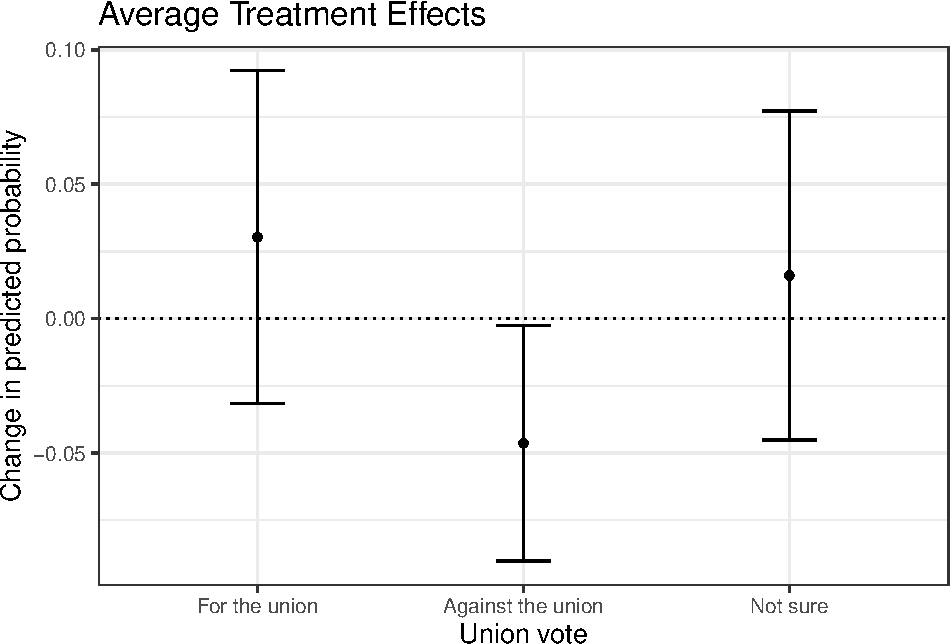
\includegraphics{EHF_Spring2025_files/figure-latex/fig-uv-models-wmt-1.pdf}
\caption{\label{fig:fig-uv-models-wmt}Treatment effect on support for unionization with 95\% confidence intervals (Walmart)}
\end{figure}

In Study 3, we also asked respondents to use a slider to indicate the percent of their co-workers they expect would vote to support unionization. Table \ref{tab:tab-usupp-models-wmt} displays the regression-estimated treatment effects. The video treatment induces a four percentage point average increase in the expected percentage, off of a baseline average of 50\%, a modest but relatively precisely estimated effect.

\begin{table}
\centering
\caption{\label{tab:tab-uv-models-wmt}OLS regression of expected union support among co-workers \label{tab:tab-usupp-models-wmt}}
\centering
\begin{threeparttable}
\begin{tabular}[t]{lccc}
\toprule
  & base & covariates & pre-exposed\\
\midrule
Treated & \num{4.173}* & \num{3.992}* & \num{4.459}\\
 & (\num{1.837}) & (\num{1.820}) & (\num{2.397})\\
Pre-exposed &  &  & \num{-0.881}\\
 &  &  & (\num{2.640})\\
Treated x pre-exposed &  &  & \num{-0.843}\\
 &  &  & (\num{3.736})\\
\midrule
$N$ & \num{980} & \num{980} & \num{980}\\
$R^2$ & \num{0.01} & \num{0.05} & \num{0.01}\\
F & \num{5.16} & \num{6.66} & \num{1.86}\\
\bottomrule
\end{tabular}
\begin{tablenotes}
\item * p $<$ 0.05, ** p $<$ 0.01 Robust standard errors in parentheses. Covariates include age, gender race, job tenure, hourly and full time status, college degree, and main job.
\end{tablenotes}
\end{threeparttable}
\end{table}

Finally, we look at social insurance policies. In the Walmart survey we again asked respondents the level of responsibility the government has for the elderly and the unemployed. To further directly examine the substitution hypothesis, I also asked respondents about government responsibility for ``people confronting short-term hardships.'' As Table\textasciitilde\ref{tab:tab-ui-hard-wmt} displays, we find no evidence of any treatment effect for any of these policy areas among Walmart workers; pre-exposure to the ACNT makes no difference in this conclusion. Across both the Home Depot and Walmart surveys, we see no evidence that ``private welfare'' in the form of EHFs has any negative effect on support for government-directed social support, whether for the unemployed, elderly, those experiencing, or the .

\begin{table}
\centering
\begin{talltblr}[         %% tabularray outer open
caption={Support for unemployment insurance and emergency government support  \label{tab:tab-ui-hard-wmt}},
note{}={* p \num{< 0.05}, ** p \num{< 0.01}},
note{ }={Robust standard errors in parentheses. Covariates include age, gender race, job tenure, hourly status, full time status, college degree, and main job.},
]                     %% tabularray outer close
{                     %% tabularray inner open
colspec={Q[]Q[]Q[]Q[]Q[]Q[]Q[]},
column{2,3,4,5,6,7}={}{halign=c,},
column{1}={}{halign=l,},
hline{8}={1,2,3,4,5,6,7}{solid, black, 0.05em},
}                     %% tabularray inner close
\toprule
& UI & UI  & UI   & Emergency & Emergency  & Emergency   \\ \midrule %% TinyTableHeader
Treated & \num{0.016} & \num{0.018} & \num{0.016} & \num{0.019} & \num{0.012} & \num{0.012} \\
& (\num{0.014}) & (\num{0.017}) & (\num{0.018}) & (\num{0.013}) & (\num{0.017}) & (\num{0.017}) \\
Pre-exposed &  & \num{0.003} & \num{0.007} &  & \num{-0.007} & \num{-0.005} \\
&  & (\num{0.020}) & (\num{0.020}) &  & (\num{0.019}) & (\num{0.020}) \\
Treated x pre-exposed &  & \num{-0.005} & \num{-0.005} &  & \num{0.017} & \num{0.014} \\
&  & (\num{0.028}) & (\num{0.028}) &  & (\num{0.027}) & (\num{0.027}) \\
Covariates? & No & No & Yes & No & No & Yes \\
$N$ & \num{980} & \num{980} & \num{980} & \num{980} & \num{980} & \num{980} \\
$R^2$ & \num{0.00} & \num{0.00} & \num{0.01} & \num{0.00} & \num{0.00} & \num{0.01} \\
$F$ & \num{1.32} & \num{0.46} & \num{1.44} & \num{2.14} & \num{0.86} & \num{1.27} \\
\bottomrule
\end{talltblr}
\end{table}

\subsection{Discussion}\label{discussion}

\subsubsection{descriptive conclusions}\label{descriptive-conclusions}

In study 1 we saw that retail workers are generally unaware of the EHFs and show limited knowledge about which employers offer these programs, suggesting that EHFs have not become a significant tool for recruiting and retain retail workers. On the other hand, the low cost and ubiquity of EHFs in retail may indicate that in equilibrium all larger employers offer EHFs and workers rationally don't pay much attention to the specifics. But the fact that respondents show strong interest in EHF programs after being told about them suggest that this interpretation is unlikely. Retail workers appear to value emergency support, at least in the abstract. And, given the choice, they would prefer workers to have some voice over the program's operation.

\subsubsection{research hypotheses}\label{research-hypotheses}

Two different surveys among Home Depot and Walmart workers present consistent as well as mixed findings around our research hypotheses. These findings are difficult to reconcile with an overarching theory of EHFs or ``private welfare,'' but, I will argue, they are consistent with differences across EHF programs, corporate cultures, and worker populations.

Across both surveys, we found that workers aware of their employers' EHFs before the survey were, in fact, more attached to their jobs, felt more financially stable, and were less likely to support unionization, even after conditioning on predictors of pre-exposure such as job tenure. But this does not warrant a causal interpretation, as the causal arrow between EHF awareness and job tenure could go either way or be the result of some omitted factor. When using a survey experiment that exploits actual employer messages to workers around EHFs, we saw that these messages produced no effect on either subjective financial security or support for public social assistance programs in both surveys, contrary to the programs' stated intent and the ``substitution hypothesis'', respectively.

There were two notable differences in treatment effects between Study 2 and Study 3. Among the Home Depot population, the video treatment substantially increased job attachment and increased uncertainty around unionization by reducing support, consistent with the research hypotheses. Both effects were concentrated among respondents who were unaware of the EHF prior to the survey, as expected. In Study 3 among Walmart workers, the EHF video had no detectable effect on job attachment and \emph{reduced} opposition to unionization while increasing the proportion of workers that respondents believed would support unionization. The video treatment increased the likelihood that a respondent would click a link to donate to the ACNT. None of these effects varied based on pre-exposure to the program.

These contrary findings suggest that the effect of EHF programs and messages depend on the nature of the program itself as well as context, perhaps including other corporate practices and signals about corporate culture. The HF is considerably more visible and generous, embedded in a significant CSR and internal promotional apparatus. Home Depot workers held more favorable attitudes towards their employer and were already more likely to engage with the EHF prior to the survey experiment. Consequently, the EHF treatment appears to have reinforced an existing set of attitudes and dispositions, making those who were unaware of the program ``look more like'' already-informed Home Depot workers in their attitudes. When looking at Walmart, it seems that an EHF program with less organizational support and visibility does not ``make up the difference'' in worker attachment between a ``strong culture, low turnover'' employer like the Home Depot and a ``weak culture, high turnover'' employer such as Walmart.

\section{Conclusion}\label{conclusion}

Employers have tremendous leeway to introduce or modify benefit plans and workplace programs that may influence workers perceptions, attitudes, and behaviors including around and politically relevant actions like unionization. EHFs are one such tax-incentivized program that has received virtually no systematic study. This oversight is all the more remarkable as EHFs clearly echo both an earlier era of welfare capitalism and past mutual aid initiatives that produced and modern labor unions.

This paper provides the first systematic glimpse into EHFs in the US retail, an industry that employs tens of millions but that is also known for low wages and elevated levels of worker churn and activism in the post-COVID period. Using original surveys, I find that between 13\% and 30\% of retail workers report having an EHF at their current job. When asked about EHFs at major retail employers, worker knowledge is limited, suggesting that EHFs have not become a significant tool for recruiting and retaining retail workers. Nevertheless, when the programs are explained, workers show strong support for them, including valuing them as highly as improved health insurance benefits when considering a hypothetical job offer. EHFs do seem to address a real need.

To better ground these findings in specific employer contexts, I used social media to recruit survey respondents who work at two large US retailers with well-established, in-house EHFs: the Home Depot and Walmart. These firms have much in common, but their EHFs differ. The Home Depot EHF is substantially more generous and more heavily promoted as part of corporate events, CSR, and training. Consistent with these differences, I found that worker awareness at the Home Depot exceeded 60\%, with large proportions claiming to have have donated. Among Walmart workers, I find just over one third of workers aware of the EHF, with less than 15\% claiming to have donated. I characterized worker awareness as ``broad-but-thin'': workers knew of an emergency grant program, but were less clear on how it functioned and its connection to worker donations. At both firms, awareness and other engagement with the EHF is strongly correlated with worker tenure, full-time status, and gender. Men were less aware and engaged.

Using survey experiments, I explored the effect employer-produced promotional video messages the EHF on subjective financial security, job attachment, donation willingness, and support for unionization and public assistance programs for the unemployed and those in temporary need. Contrary to expectations and stated EHF goals, I found no evidence in either survey that the EHF treatments induce any improvement in worker's subjective financial security, although workers who were aware of the program before the survey experiment were systematically more positive about their financial situation.

Findings related to the ``substitution hypothesis''--the claim that private benefits and resources reduce support for government-provided programs--were another area of agreement across Studies 2 and 3. Specifically, the video treatment shows no evidence of a negative effect on respondent support for government unemployment insurance or aid to those in temporary hardship. In the Home Depot sample, the treatment induced a modest but significant \emph{increase} in support for government-provided UI. This outcome may be the result of Home Depot workers having a better understanding of the EHF program (and its limitations). Findings in these surveys are inconsistent with a simple ``private options crowd out public benefits'' story.

Findings for job attachment diverged across cases. At the Home Depot, the video treatment had the expected positive effect, consistent with past work on CSR initiatives and employee motivation and retention (\citeproc{ref-burbanoGettingGigWorkers2021}{Burbano 2021}). When we disaggregated these effects, we found that the treatment effects were largely concentrated among the respondents who were unaware of the EHF before the survey. At Walmart, we found no treatment effect on job attachment.

Looking at support for unionization, we uncovered an even starker pattern. At the Home Depot, the video treatment caused significant decrease in support for unionization of about 10 percentage points among those unaware of the EHF before the survey, but no effect among the pre-exposed (who were more anti-union on average). By examining the full range of outcome values, we also saw that this decrease in support for unionization came through an increase in \emph{uncertainty} about unions, as opposed to an increase in outright opposition. This suggests that EHFs could be used to demobilize workers, especially newer hires, during a unionization campaign. At Walmart, however, we found that the EHF treatment significantly reduced opposition to unionization by about four percentage points; prior knowledge of the EHF was unrelated to treatment effects. We also found that the video treatment increased Walmart workers' expectations about their co-workers willingness to vote for a union as well as likelihood of taking an action to donate to the EHF.

Taken together, these patterns are consistent with the claim---articulated by EHF managers themselves---that EHF programs serve a culture-building and retention function at relatively low cost. Calling attention to the EHF in the context of broader CSR and team building, as the Home Depot does, has the effect of shifting opinion of newer and arguably more mobile workers in the direction of those who have been around longer. At Walmart, however, the EHF program has enjoyed less organizational support and visibility. I find that similar EHF messaging fails to resonate as strongly with workers.

EHFs present a fascinating window into employer behavior and the state of the low wage labor market in the US and beyond. Future research can extend in a variety of productive directions. One obvious area connects with consumers: do programs of this kind affect consumers' perception of corporate brands and their labor practices? Another involves timing: are EHFs (and communication around them) more likely during periods of elevated worker leverage or union activity? Can we document and explain which firms develop EHFs? How do companies operating across borders view and manage EHFs and similar ``private welfare'' initiatives?

From a policy perspective, EHFs appear resonate with a felt need among low-wage retail workers in the US today. But, as the Home Depot and Walmart surveys indicate, program details, context, and promotion matter for the effects they might have on the workforce. These programs operate in the shadow of eroded public welfare institutions, yet they are funded in part by favorable tax treatment. Are the benefits these programs provide worth the tax expenditures? How do these programs change when workers themselves have a voice in how they are run?

\section*{References}\label{references}
\addcontentsline{toc}{section}{References}

\phantomsection\label{refs}
\begin{CSLReferences}{1}{0}
\bibitem[\citeproctext]{ref-abraham_measuring_2018}
Abraham, Katherine G., John C. Haltiwwanger, Kristen Sandusky, and James Spletzer. 2018. \emph{Measuring the {Gig} {Economy}: Current Knowledge and Open Issues}. 24950. NBER.

\bibitem[\citeproctext]{ref-socialsecurityadministrationSocialSecurityHistory2023}
Administration, Social Security. 2023. {``Social {Security History}.''} https://www.ssa.gov/history/reports/ces/cesbookc1.html.

\bibitem[\citeproctext]{ref-ahlquist_ARPS_2017}
Ahlquist, John S. 2017. {``Labor Unions, Political Representation, and Economic Inequality.''} \emph{Annual Review of Political Science} 20 (1): 409--32.

\bibitem[\citeproctext]{ref-ahlquist_research_2018}
---------. 2018. {``Research {Frontiers} in the {Institutional} {Analysis} of {Work}.''} In \emph{The {Research} {Agenda} for {New} {Institutional} {Economics}}, edited by Claude Menard and Mary Shirley. Elsevier.

\bibitem[\citeproctext]{ref-AGT_youngworkers}
Ahlquist, John S., Jacob M. Grumbach, and Eric Thai. 2023. {``Voice on the Job for Younger Workers.''} Research report. Annie E. Casey Foundation; UC San Diego.

\bibitem[\citeproctext]{ref-ahlquist_interest_2013}
Ahlquist, John S., and Margaret Levi. 2013. \emph{In the {Interest} of {Others}: Organizations and Social Activism}. Princeton: Princeton University Press.

\bibitem[\citeproctext]{ref-ahlquist_firm_2020}
Ahlquist, John S., and Layna Mosley. 2021. {``Firm Participation in Voluntary Regulatory Initiatives: {The} {Accord}, {Alliance}, and {US} Garment Importers from {Bangladesh}.''} \emph{The Review of International Organizations} 16 (317-343). \url{https://doi.org/10.1007/s11558-020-09376-z}.

\bibitem[\citeproctext]{ref-akerlof_theory_1980}
Akerlof, George A. 1980. {``A {Theory} of {Social} {Custom}, of Which {Unemployment} May Be {One} {Consequence}.''} \emph{The Quarterly Journal of Economics} 94 (4): 749--75. \url{https://doi.org/10.2307/1885667}.

\bibitem[\citeproctext]{ref-amorim_schedule_2022}
Amorim, Mariana, and Daniel Schneider. 2022. {``Schedule {Unpredictability} and {High}-{Cost} {Debt}: {The} {Case} of {Service} {Workers}.''} \emph{Sociological Science} 9 (April): 102--35. \url{https://doi.org/10.15195/v9.a5}.

\bibitem[\citeproctext]{ref-anderson_private_2017}
Anderson, Elizabeth. 2017. \emph{Private {Government}}. Princeton, NJ: Princeton University Press. \url{https://press.princeton.edu/books/hardcover/9780691176512/private-government}.

\bibitem[\citeproctext]{ref-andreoniPowerAskingHow2011}
Andreoni, James, and Justin M. Rao. 2011. {``The Power of Asking: {How} Communication Affects Selfishness, Empathy, and Altruism.''} \emph{Journal of Public Economics} 95 (7-8): 513--20. \url{https://doi.org/10.1016/j.jpubeco.2010.12.008}.

\bibitem[\citeproctext]{ref-ansell_political_2014}
Ansell, Ben. 2014. {``The {Political} {Economy} of {Ownership}: {Housing} {Markets} and the {Welfare} {State}.''} \emph{American Political Science Review} 108 (2): 383--402. \url{https://doi.org/10.1017/S0003055414000045}.

\bibitem[\citeproctext]{ref-aprill_charitable_2016}
Aprill, Ellen P. 2016. {``Charitable {Class}, {Disaster} {Relief}, and {First} {Responders}.''} \{SSRN\} \{Scholarly\} \{Paper\} ID 2884244. Rochester, NY: Social Science Research Network. \url{https://papers.ssrn.com/abstract=2884244}.

\bibitem[\citeproctext]{ref-aspen_institute_illuminating_2019}
Aspen Institute. 2019. {``Illuminating a {Hidden} {Safety} {Net}: {Lessons} from {Research} into {Employee} {Hardship} {Funds}.''} Aspen Institute. \url{https://www.aspeninstitute.org/publications/illuminating-a-hidden-safety-net-lessons-from-research-into-employee-hardship-funds/}.

\bibitem[\citeproctext]{ref-noauthor_environmental_2013}
Association of Disaster Relief Funds and Employee Hardship Funds. 2013. {``An {Environmental} {Scan} of {Disaster} {Relief} and {Employee} {Hardship} {Funds}.''}

\bibitem[\citeproctext]{ref-bacharach_mutual_2018}
Bacharach, Samuel B., Peter A. Bamberger, and William J. Sonnenstuhl. 2018. \emph{Mutual {Aid} and {Union} {Renewal}: {Cycles} of {Logics} of {Action}}. Cornell University Press. \url{https://www.degruyter.com/view/title/552290}.

\bibitem[\citeproctext]{ref-beito_mutual_2000}
Beito, David T. 2000. \emph{From {Mutual} {Aid} to the {Welfare} {State}: {Fraternal} {Societies} and {Social} {Services}, 1890-1967}. Chapel Hill: University of North Carolina Press.

\bibitem[\citeproctext]{ref-SHED2022}
Board of Governors of the Federal Reserve System. 2023. {``Economic {Well-Being} of {U}.{S}. {Households} in 2022.''} {US Federal Reserve}.

\bibitem[\citeproctext]{ref-bodeCorporateSocialInitiatives2015}
Bode, Christiane, Jasjit Singh, and Michelle Rogan. 2015. {``Corporate {Social Initiatives} and {Employee Retention}.''} \emph{Organization Science} 26 (6): 1702--20. \url{https://www.jstor.org/stable/43663678}.

\bibitem[\citeproctext]{ref-brandesAmericanWelfareCapitalism1976}
Brandes, Stuart D. 1976. \emph{American {Welfare Capitalism}}. Chicago: University of Chicago Press.

\bibitem[\citeproctext]{ref-bronfenbrenner_2009}
Bronfenbrenner, Kate. 2009. {``No Holds Barred: The Intensification of Employer Opposition to Organizing.''} Economic Policy Institute.

\bibitem[\citeproctext]{ref-burbanoGettingGigWorkers2021}
Burbano, Vanessa C. 2021. {``Getting {Gig Workers} to {Do More} by {Doing Good}: {Field Experimental Evidence From Online Platform Labor Marketplaces}.''} \emph{Organization \& Environment} 34 (3): 387--412. \url{https://doi.org/10.1177/1086026619846455}.

\bibitem[\citeproctext]{ref-busemeyer_welfare_2020}
Busemeyer, Marius R., and Torben Iversen. 2020. {``The {Welfare} {State} with {Private} {Alternatives}: The Transformation of Popular Support for Social Insurance.''} \emph{Journal of Politics}.

\bibitem[\citeproctext]{ref-corporatephilanthropyexecutiveatanapparelcompanyEHFInterview12024}
Corporate philanthropy executive at an apparel company. 2024. {``{EHF} Interview \#1.''}

\bibitem[\citeproctext]{ref-derickson_workers_1988}
Derickson, Alan. 1988. \emph{Workers' {Health}, {Workers}' {Democracy}: {The} {Western} {Miners}' {Struggle}, 1891-1925}. Ithaca: Cornell University Press.

\bibitem[\citeproctext]{ref-distelhorst_does_2017}
Distelhorst, Greg, Jens Hainmueller, and Richard M. Locke. 2017. {``Does {Lean} {Improve} {Labor} {Standards}? {Management} and {Social} {Performance} in the {Nike} {Supply} {Chain}.''} \emph{Management Science} 63 (3): 707--28. \url{https://doi.org/10.1287/mnsc.2015.2369}.

\bibitem[\citeproctext]{ref-dreyfus_labour_1993}
Dreyfus, Michel. 1993. {``The Labour Movement and Mutual Benefit Societies: {Towards} an International Approach.''} \emph{International Social Security Review} 46 (3): 19--27. \url{https://doi.org/10.1111/j.1468-246X.1993.tb00381.x}.

\bibitem[\citeproctext]{ref-employee_relief_fund_education_group_environmental_2019}
Employee Relief Fund Education Group. 2019. {``An {Environmental} {Scan} of {Disaster} {Relief} and {Employee} {Hardship} {Funds}.''} The Employee Relief Fund Education Group. \url{https://emergencyassistancefdn.org/white-paper/}.

\bibitem[\citeproctext]{ref-executiveatehfthirdpartyproviderEHFInterview22024}
Executive at EHF third party provider. 2024. {``{EHF} Interview \#2.''}

\bibitem[\citeproctext]{ref-executiveatehfthirdpartyproviderEHFInterview52025}
Executive at EHF third party provider, leader. 2025. {``{EHF} Interview \#5.''}

\bibitem[\citeproctext]{ref-ferrariMethodologicalApproachCausal2023}
Ferrari, Diogo. 2023. {``A {Methodological Approach} for {Causal Inference} Under {Uncontrolled} (and {Possibly Latent}) {Pre-exposure} to {Treatment}.''} Working \{\{Paper\}\}.

\bibitem[\citeproctext]{ref-fothergill_stigma_2003}
Fothergill, Alice. 2003. {``The {Stigma} of {Charity}:''} \emph{The Sociological Quarterly} 44 (4): 659--80. \url{https://doi.org/10.1111/j.1533-8525.2003.tb00530.x}.

\bibitem[\citeproctext]{ref-employeeassistancefoundationDecadeAssistanceOffering2022}
Foundation, Employee Assistance. 2022. {``A {Decade} of {Assistance}: Offering Hope Through Disaster and Hardship Relief Funds.''}

\bibitem[\citeproctext]{ref-glenn_understanding_2001}
Glenn, Brian J. 2001. {``Understanding {Mutual} {Benefit} {Societies}, 1860-1960.''} \emph{Journal of Health Politics, Policy, and Law} 26 (3): 638--51.

\bibitem[\citeproctext]{ref-godfreyRelationshipCorporateSocial2009}
Godfrey, Paul C., Craig B. Merrill, and Jared M. Hansen. 2009. {``The Relationship Between Corporate Social Responsibility and Shareholder Value: An Empirical Test of the Risk Management Hypothesis.''} \emph{Strategic Management Journal} 30 (4): 425--45. \url{https://doi.org/10.1002/smj.750}.

\bibitem[\citeproctext]{ref-gorton_corporate_2020}
Gorton, Gary B, and Alexander K Zentefis. 2020. {``Corporate {Culture} as a {Theory} of the {Firm}.''} Working \{Paper\} 27353. NBER.

\bibitem[\citeproctext]{ref-greeningCorporateSocialPerformance2000}
Greening, Daniel W., and Daniel B. Turban. 2000. {``Corporate {Social Performance As} a {Competitive Advantage} in {Attracting} a {Quality Workforce}.''} \emph{Business \& Society} 39 (3): 254--80. \url{https://doi.org/10.1177/000765030003900302}.

\bibitem[\citeproctext]{ref-grow_is_nodate}
Grow, André, Daniela Perrotta, Emanuele Del Fava, Jorge Cimentada, Francesco Rampazzo, Sofia Gil-Clavel, Emilio Zagheni, René D. Flores, Ilana Ventura, and Ingmar Weber. forthcoming. {``Is {Facebook}'s Advertising Data Accurate Enough for Use in Social Science Research? {Insights} from a Cross-National Online Survey.''} \emph{Journal of the Royal Statistical Society: Series A} n/a (n/a). \url{https://doi.org/10.1111/rssa.12948}.

\bibitem[\citeproctext]{ref-hacker_great_2019}
Hacker, Jacob S. 2019. \emph{The {Great} {Risk} {Shift}: {The} {New} {Economic} {Insecurity} and the {Decline} of the {American} {Dream}, {Second} {Edition}}. Second Edition. New York: Oxford University Press.

\bibitem[\citeproctext]{ref-hacker_insecure_2013}
Hacker, Jacob S., Philipp Rehm, and Mark Schlesinger. 2013. {``The {Insecure} {American}: {Economic} {Experiences}, {Financial} {Worries}, and {Policy} {Attitudes}.''} \emph{Perspectives on Politics} 11 (1): 23--49. \url{https://doi.org/10.1017/S1537592712003647}.

\bibitem[\citeproctext]{ref-hayton_little_2012}
Hayton, James C., Gianluca Carnabuci, and Robert Eisenberger. 2012. {``With a Little Help from My Colleagues: {A} Social Embeddedness Approach to Perceived Organizational Support.''} \emph{Journal of Organizational Behavior} 33 (2): 235--49. \url{https://doi.org/10.1002/job.755}.

\bibitem[\citeproctext]{ref-herd_administrative_2019}
Herd, Pamela, and Donald P. Moynihan. 2019. \emph{Administrative {Burden}: {Policymaking} by {Other} {Means}}. 1st edition. New York: Russell Sage Foundation.

\bibitem[\citeproctext]{ref-hertel-fernandez_why_nodate}
Hertel-Fernandez, Alexander, and Ethan Porter. 2021. {``Why {Public} {Sector} {Union} {Members} {Support} {Their} {Unions}: {Survey} and {Experimental} {Evidence}.''} \emph{Social Forces} 100 (1): 375--99. \url{https://doi.org/10.1093/sf/soaa087}.

\bibitem[\citeproctext]{ref-horowitz_mutualism_2021}
Horowitz, Sara. 2021. \emph{Mutualism: {Building} the {Next} {Economy} from the {Ground} {Up}}. New York: Penguin Random House.

\bibitem[\citeproctext]{ref-humanresourcesandpayrolladministratoratalargeretailerEHFInterview42024}
Human resources and payroll administrator at a large retailer. 2024. {``{EHF} Interview \#4.''}

\bibitem[\citeproctext]{ref-noauthor_disaster_2014}
Internal Revenue Service. 2014. {``Disaster {Relief}: Providing Assistance Through Charitable Organizations.''} 3833 (Rev. 12-2014). Internal Revenue Service.

\bibitem[\citeproctext]{ref-ismay_trust_2018}
Ismay, Penelope. 2018. \emph{Trust {Among} {Strangers}: {Friendly} {Societies} in {Modern} {Britain}}. Cambridge: Cambridge University Press. \url{https://doi.org/10.1017/9781108560535}.

\bibitem[\citeproctext]{ref-jacobyModernManorsWelfare1998}
Jacoby, Sanford M. 1998. \emph{Modern {Manors}: {Welfare Capitalism} Since the {New Deal}}. Princeton: Princeton University Press.

\bibitem[\citeproctext]{ref-jarley_unions_2005}
Jarley, Paul. 2005. {``Unions as {Social} {Capital}: {Renewal} Through a {Return} to the {Logic} of {Mutual} {Aid}?''} \emph{Labor Studies Journal} 29 (4): 1--26. \url{https://doi.org/10.1353/lab.2005.0011}.

\bibitem[\citeproctext]{ref-kampkotter_employee_2020}
Kampkötter, Patrick, Lea Petters, and Dirk Sliwka. 2020. {``Employee {Identification} and {Wages}: {On} the {Economics} of {``}{Affective} {Commitment}{''}.''} 13624. IZA.

\bibitem[\citeproctext]{ref-kochan_us_2022}
Kochan, Thomas A., Janice Fine, Kate Bronfenbrenner, Suresh Naidu, Jacob Barnes, Yaminette Diaz-Linhart, Johnnie Kallas, et al. 2022. {``U.{S}. {Workers}{'} {Organizing} {Efforts} and {Collective} {Actions}: {A} {Review} of the {Current} {Landscape}.''} Worker Empowerment Research network (WERN). \url{https://iwer.mit.edu/wp-content/uploads/2022/06/Report-on-Worker-Organizing-Landscape-in-US-by-Kochan-Fine-Bronfenbrenner-Naidu-et-al-June-2022.pdf}.

\bibitem[\citeproctext]{ref-kochan_worker_2019}
Kochan, Thomas A., Duanyi Yang, William T. Kimball, and Erin L. Kelly. 2019. {``Worker {Voice} in {America}: {Is} {There} a {Gap} Between {What} {Workers} {Expect} and {What} {They} {Experience}?''} \emph{ILR Review} 72 (1): 3--38. \url{https://doi.org/10.1177/0019793918806250}.

\bibitem[\citeproctext]{ref-landis_fate_1999}
Landis, Michele L. 1999. {``Fate, {Responsibility}, and "{Natural}" {Disaster} {Relief}: {Narrating} the {American} {Welfare} {State}.''} \emph{Law \& Society Review} 33 (2): 257--318. \url{https://doi.org/10.2307/3115166}.

\bibitem[\citeproctext]{ref-lecyNCCSIRS9902023}
Lecy, Jesse D. 2023. {``{NCCS IRS} 990 {Efile Data}.''}

\bibitem[\citeproctext]{ref-lin_modeling_2010}
Lin, Chieh-Peng. 2010. {``Modeling {Corporate} {Citizenship}, {Organizational} {Trust}, and {Work} {Engagement} {Based} on {Attachment} {Theory}.''} \emph{Journal of Business Ethics} 94 (4): 517--31. \url{https://doi.org/10.1007/s10551-009-0279-6}.

\bibitem[\citeproctext]{ref-locke_promise_2013}
Locke, Richard M. 2013. \emph{The {Promise} and {Limits} of {Private} {Power}: {Promoting} {Labor} {Standards} in a {Global} {Economy}}. Cambridge {Studies} in {Comparative} {Politics}. Cambridge: Cambridge University Press. \url{https://doi.org/10.1017/CBO9781139381840}.

\bibitem[\citeproctext]{ref-malesky_chains_2018}
Malesky, Edmund J., and Layna Mosley. 2018. {``Chains of {Love}? {Global} {Production} and the {Firm}-{Level} {Diffusion} of {Labor} {Standards}.''} \emph{American Journal of Political Science} 62 (3): 712--28. \url{https://doi.org/10.1111/ajps.12370}.

\bibitem[\citeproctext]{ref-maretingandcommunicationexecutiveatehfthirdpartyproviderEHFInterview32024}
Mareting and communication executive at EHF third party provider. 2024. {``{EHF} Interview \#3.''}

\bibitem[\citeproctext]{ref-Gallup_unions_2022}
McCarthy, Justin. 2022. {``U.s. Approval of Labor Unions at Highest Point Since 1965.''}

\bibitem[\citeproctext]{ref-morrisCriminalConspiracyEarly1937}
Morris, Richard B. 1937. {``Criminal {Conspiracy} and {Early Labor Combinations} in {New York}.''} \emph{Political Science Quarterly} 52 (1): 51--85. \url{https://doi.org/10.2307/2143898}.

\bibitem[\citeproctext]{ref-naidu_is_nodate}
Naidu, Suresh. 2022. {``Is There Any Future for a {US} {Labor} {Movement}?''} \emph{Journal of Economic Perspectives} 36 (4): 3--28.

\bibitem[\citeproctext]{ref-naylor_economic_1993}
Naylor, Robin, and Martin Cripps. 1993. {``An Economic Theory of the Open Shop Trade Union.''} \emph{European Economic Review} 37 (8): 1599--1620. \url{https://doi.org/10.1016/0014-2921(93)90123-R}.

\bibitem[\citeproctext]{ref-neumannWhereHaveAll1984}
Neumann, George R., and Ellen R. Rissman. 1984. {``Where {Have All} the {Union Members Gone}?''} \emph{Journal of Labor Economics} 2 (2): 175--92. \url{https://www.jstor.org/stable/2534894}.

\bibitem[\citeproctext]{ref-olson_logic_1965}
Olson, Mancur. 1965. \emph{The {Logic} of {Collective} {Action}}. Cambridge, MA: Harvard University Press.

\bibitem[\citeproctext]{ref-parsell_clarke_2022}
Parsell, Cameron, and Andrew Clarke. 2022. {``Charity and Shame: Towards Reciprocity.''} \emph{Social Problems} 69 (2): 436--52.

\bibitem[\citeproctext]{ref-putnam_making_1994}
Putnam, Robert D. 1994. \emph{Making {Democracy} {Work}: {Civic} {Traditions} in {Modern} {Italy}}. 1st edition. Princeton, NJ: Princeton University Press.

\bibitem[\citeproctext]{ref-quadagno_transformation_1988}
Quadagno, Jill. 1988. \emph{The {Transformation} of {Old} {Age} {Security}: {Class} and {Politics} in the {American} {Welfare} {State}}. Chicago: University of Chicago Press.

\bibitem[\citeproctext]{ref-reich_working_2018}
Reich, Adam, and Peter Bearman. 2018. \emph{Working for {Respect}: {Community} and {Conflict} at {Walmart}}. Columbia University Press. \url{https://www.jstor.org/stable/10.7312/reic18842}.

\bibitem[\citeproctext]{ref-rodriguez_creating_2020}
Rodriguez, Jenny Calvert. 2020a. {``Creating a {Safety} {Net}: {Employee} {Hardship} {Fund} {Playbook}.''} Red Tab Foundation.

\bibitem[\citeproctext]{ref-rodriguez_every_2020}
---------. 2020b. {``Every {Company} {Should} {Have} an {Employee} {Hardship} {Fund}.''} \emph{Harvard Business Review}, no. May 21. \url{https://hbr.org/2020/05/every-company-should-have-an-employee-hardship-fund}.

\bibitem[\citeproctext]{ref-rosenTradeUnionPower1969}
Rosen, S. 1969. {``Trade {Union Power}, {Threat Effects} and the {Extent} of {Organization}.''} \emph{The Review of Economic Studies} 36 (2): 185--96. \url{https://doi.org/10.2307/2296836}.

\bibitem[\citeproctext]{ref-rosner_struggle_2003}
Rosner, David, and Gerald Markowitz. 2003. {``The {Struggle} over {Employee} {Benefits}: {The} {Role} of {Labor} in {Influencing} {Modern} {Health} {Policy}.''} \emph{The Milbank Quarterly} 81 (1): 45--73. \url{https://doi.org/10.1111/1468-0009.00038}.

\bibitem[\citeproctext]{ref-ruppEmployeeReactionsCorporate2006}
Rupp, Deborah E., Jyoti Ganapathi, Ruth V. Aguilera, and Cynthia A. Williams. 2006. {``Employee {Reactions} to {Corporate Social Responsibility}: {An Organizational Justice Framework}.''} \emph{Journal of Organizational Behavior} 27 (4): 537--43. \url{https://www.jstor.org/stable/4093915}.

\bibitem[\citeproctext]{ref-schneider_whats_2019}
Schneider, Daniel, and Kristen Harknett. 2019. {``What's to {Like}? {Facebook} as a {Tool} for {Survey} {Data} {Collection}.''} \emph{Sociological Methods \& Research}, November. \url{https://doi.org/10.1177/0049124119882477}.

\bibitem[\citeproctext]{ref-seniorexecutiveatamidsizehealthservicesfirmEHFInterview62025}
Senior executive at a midsize health services firm, leader. 2025. {``{EHF} Interview \#6.''}

\bibitem[\citeproctext]{ref-suozzoProPublicaNonprofitExplorer2025}
Suozzo, Andrea, Alec Glassford, Ash Ngu, and Brandon Roberts. 2025. {``{ProPublica Nonprofit Explorer}.''}

\bibitem[\citeproctext]{ref-taschereau-dumouchelUnionThreat2020}
Taschereau-Dumouchel, Mathieu. 2020. {``The {Union Threat}.''} \emph{The Review of Economic Studies} 87 (6): 2859--92. \url{https://doi.org/10.1093/restud/rdaa027}.

\bibitem[\citeproctext]{ref-THD_AR_2022}
The Home Depot. 2023a. {``2022 Annual Report.''} Corporate report.

\bibitem[\citeproctext]{ref-THD_ESG_2022}
---------. 2023b. {``2023 Environmental, Social, and Governance Report: Doing Our Part.''} Corporate report.

\bibitem[\citeproctext]{ref-thelen_american_2019}
Thelen, Kathleen. 2019. {``The {American} {Precariat}: {U}.{S}. {Capitalism} in {Comparative} {Perspective}.''} \emph{Perspectives on Politics} 17 (1): 5--27. \url{https://doi.org/10.1017/S1537592718003419}.

\bibitem[\citeproctext]{ref-walmartaccociatesincriticalneedtrustACNTFiscalYear2020}
Walmart Accociates in Critical Need Trust. 2020. {``{ACNT Fiscal Year} 2019 {Annual Report}: {Stand} Together Through Tough Times.''} Bentonville, AR: The Wal-Mart Associates in Critical Need Fund.

\bibitem[\citeproctext]{ref-webb_history_1920}
Webb, Sidney, and Beatrice Potter Webb. 1920. \emph{The History of Trade Unionism}. New York : Longmans, Green.

\bibitem[\citeproctext]{ref-weil_fissured_2014}
Weil, David. 2014. \emph{The {Fissured} {Workplace}}. Cambridge, MA: Harvard University Press.

\bibitem[\citeproctext]{ref-western_1997}
Western, Bruce. 1997. \emph{Between Class and Market}. Princeton: Princeton University Press.

\bibitem[\citeproctext]{ref-wiedemann_how_2022}
Wiedemann, Andreas. 2022. {``How {Credit} {Markets} {Substitute} for {Welfare} {States} and {Influence} {Social} {Policy} {Preferences}: {Evidence} from {US} {States}.''} \emph{British Journal of Political Science}, 1--21. \url{https://doi.org/10.1017/S0007123420000708}.

\bibitem[\citeproctext]{ref-williamson_stigma_1974}
Williamson, John B. 1974. {``The {Stigma} of {Public} {Dependency}: {A} {Comparison} of {Alternative} {Forms} of {Public} {Aid} to the {Poor}.''} \emph{Social Problems} 22 (2): 213--28. \url{https://doi.org/10.2307/799760}.

\bibitem[\citeproctext]{ref-WERNsurvey2023}
Workers Empowerment Research Network. 2023. {``Worker Voice: Survey of Workers in Five Industries.''} Dataset.

\bibitem[\citeproctext]{ref-yeo_working_1979}
Yeo, S. 1979. {``Working Class Association, Private Capital, Welfare and the State in the Late-Nineteenth and Twentieth Centuries.''} In \emph{Social Work, Welfare and the State}, edited by N. Parry, M. Rustin, and C. Satyamurti, 48--71. London.

\bibitem[\citeproctext]{ref-zhu_policy_2015}
Zhu, Ling, and Christine S. Lipsmeyer. 2015. {``Policy Feedback and Economic Risk: The Influence of Privatization on Social Policy Preferences.''} \emph{Journal of European Public Policy} 22 (10): 1489--1511. \url{https://doi.org/10.1080/13501763.2015.1031159}.

\end{CSLReferences}

\newpage

\appendix


\section{Home Depot suggested Homer Fund contribution rates}\label{home-depot-suggested-homer-fund-contribution-rates}

\begin{figure}
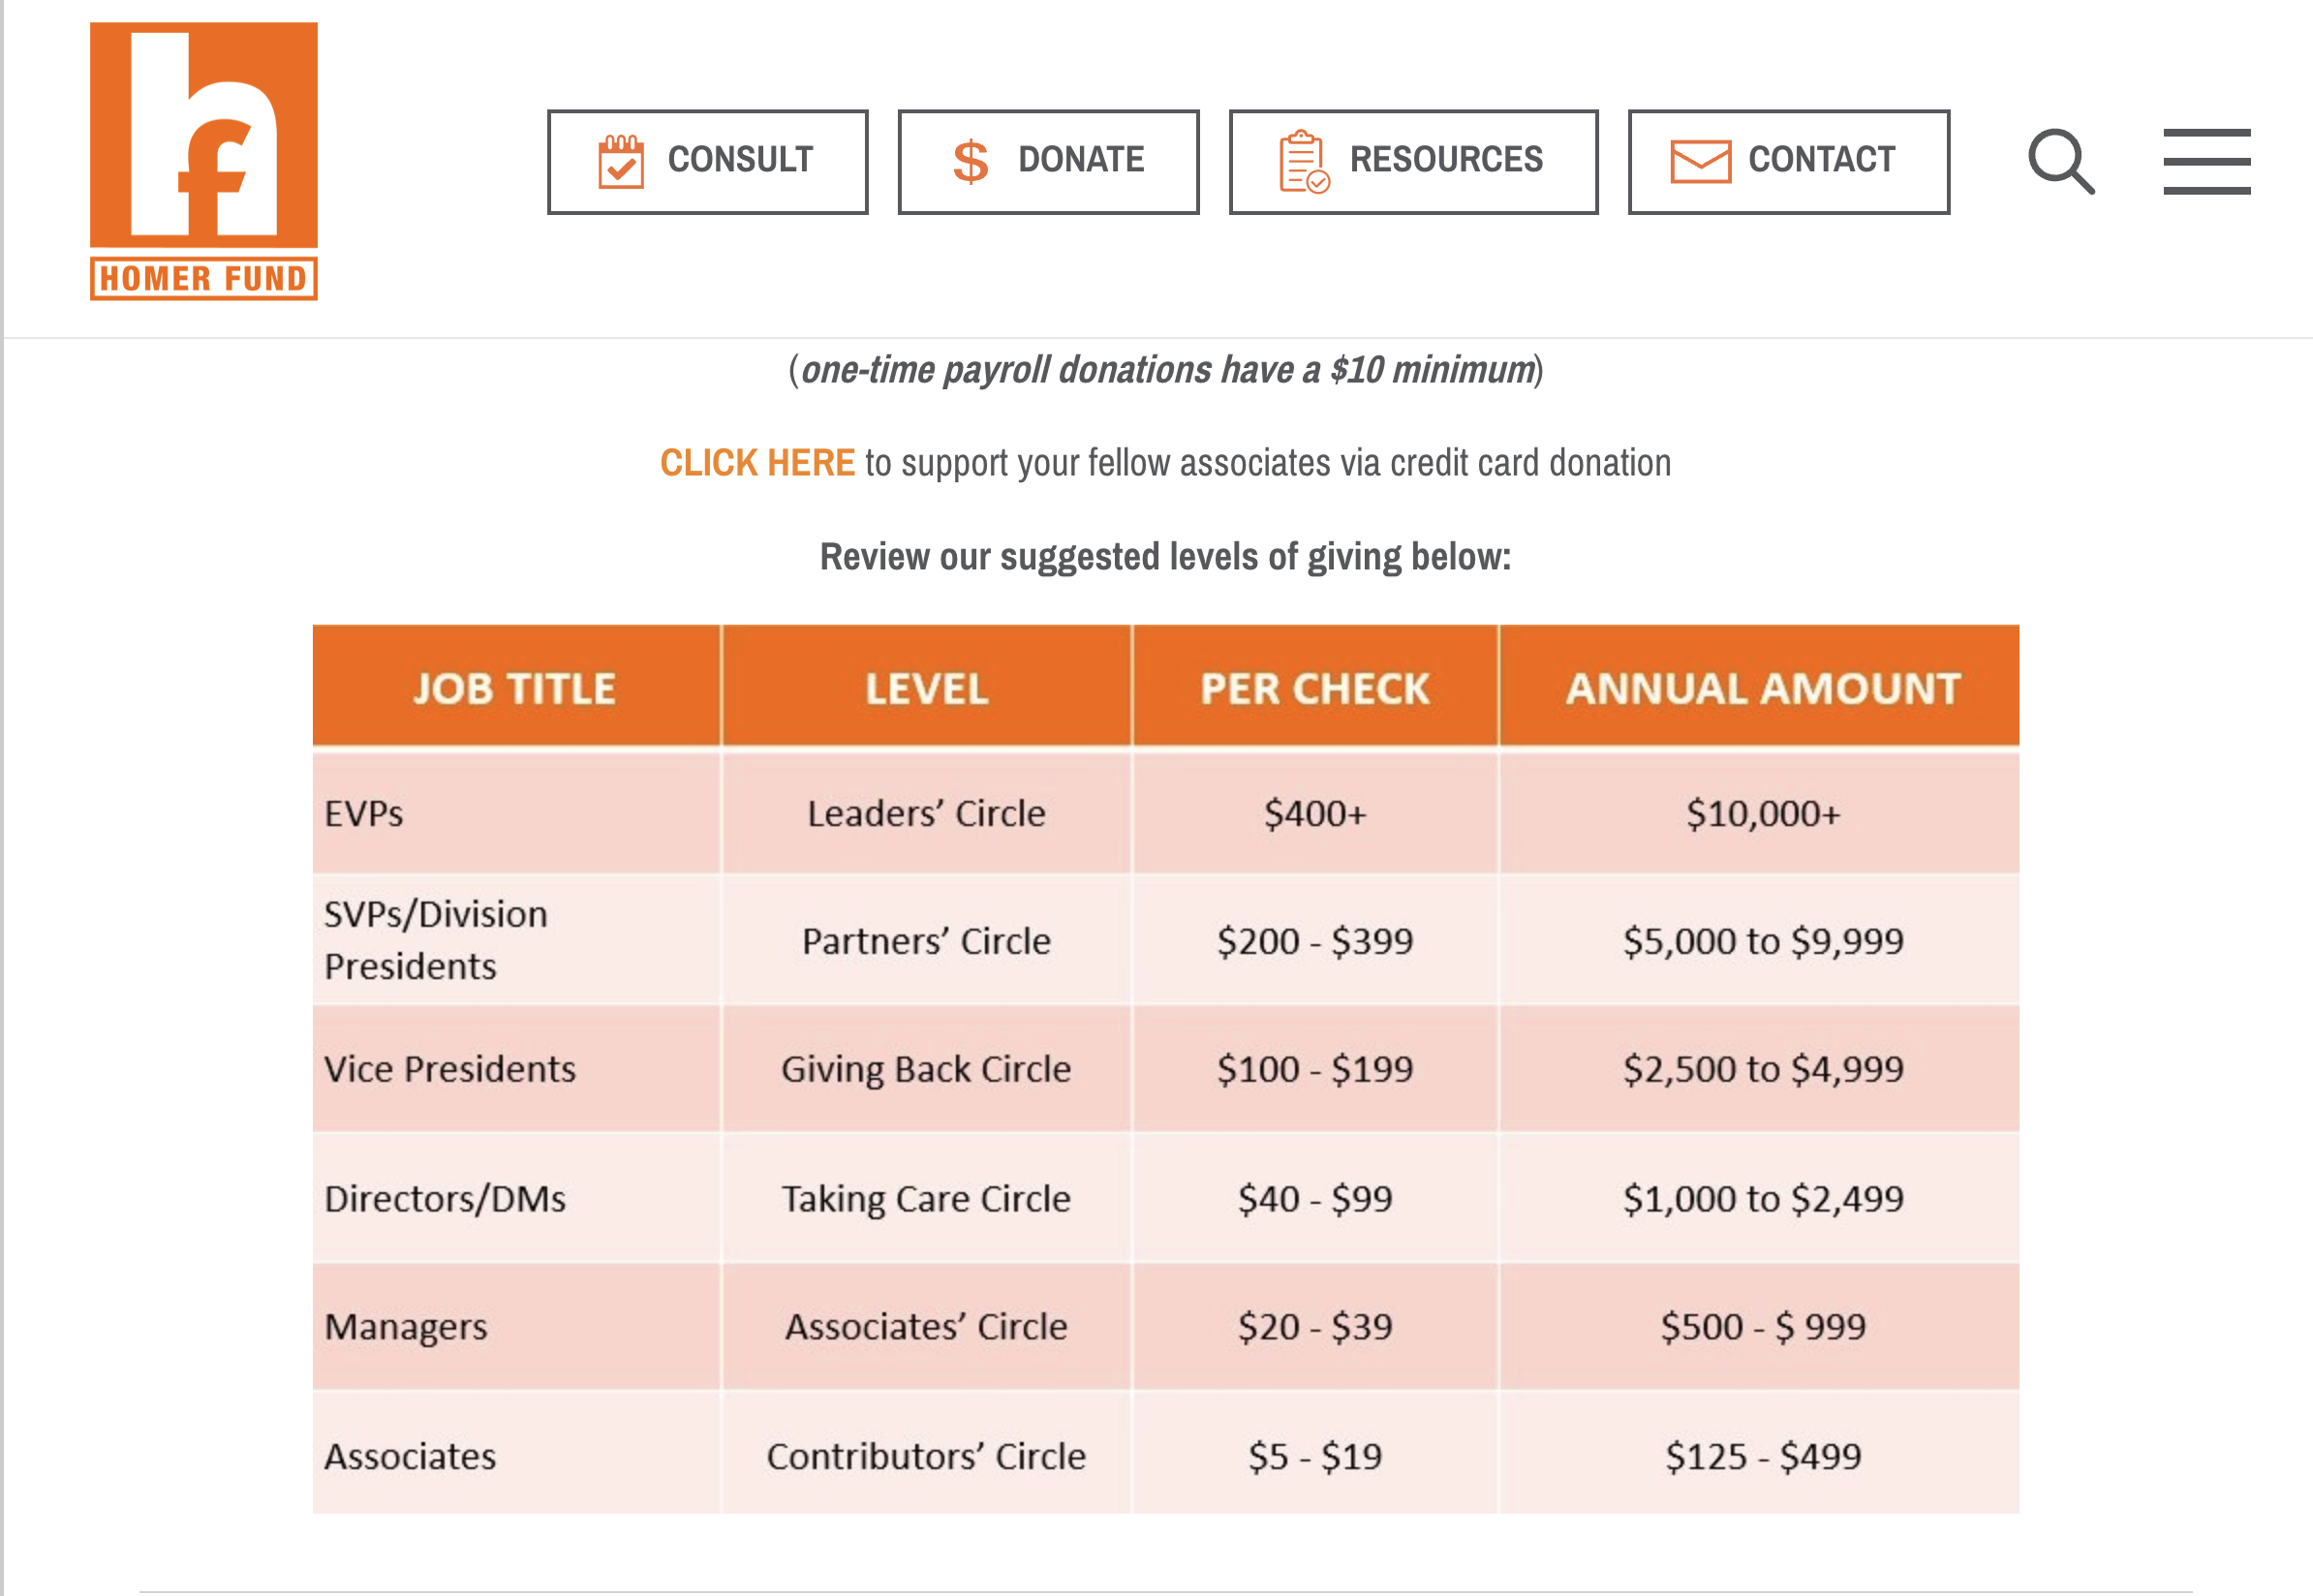
\includegraphics[width=0.6\linewidth]{plots/HF_donation_suggestions} \caption{Image of the video treatment}\label{fig:fig-sugdon}
\end{figure}

\section{Quotations from interviews}\label{app-interviews}

\subsection{Executive-driven initiative}\label{executive-driven-initiative}

\begin{quote}
``In the late 90s, after a hurricane came through\ldots the CEO at the time wanted to know why we weren't, you know, doing something for the employees. And so my, um, my boss\ldots did the research into it and kind of got a good understanding of how it would work and, uh, basically helped write the bylaws and, um, protocols around how we would issue grants.'' (\citeproc{ref-humanresourcesandpayrolladministratoratalargeretailerEHFInterview42024}{Human resources and payroll administrator at a large retailer 2024})
\end{quote}

\begin{quote}
``I think {[}executives and owners{]} felt like investing in the {[}EHF{]} was a way for them to alleviate a little bit of the pain for the workforce that they were laying off sort of en masse in the late 90s and early'' (\citeproc{ref-corporatephilanthropyexecutiveatanapparelcompanyEHFInterview12024}{Corporate philanthropy executive at an apparel company 2024})
\end{quote}

\begin{quote}
``My mom's a social worker. So a lot a lot of you know, so social, oriented professionals in my family. So that that's been my dinner table my whole life. And so that's that's really where {[}my desire to start a hardship fund{]} stems from.'' (\citeproc{ref-seniorexecutiveatamidsizehealthservicesfirmEHFInterview62025}{Senior executive at a midsize health services firm 2025})
\end{quote}

\subsection{Corporate culture}\label{corporate-culture}

\begin{quote}
``When our founder, Sam Walton, began the now-famous tradition of ``passing the hat'' at Saturday Morning Meetings years ago, he laid the foundation for a culture of caring and giving back to fellow associates. It's a tradition that endures today through the Associates in Critical Need Trust (ACNT).'' (\citeproc{ref-walmartaccociatesincriticalneedtrustACNTFiscalYear2020}{Walmart Accociates in Critical Need Trust 2020}), 4
\end{quote}

\begin{quote}
``The values are incredibly authentic and ingrained in the company\ldots this is the proof point of our
corporate value of empathy. And it's very much the center of the culture\ldots We have a eligible on day one rule for current employees. It doesn't matter how many hours a week you work or what your status is, as long as you're directly employed by the company\ldots we have a fair number of franchisees and third party affiliates\ldots that we don't and can't serve.'' (\citeproc{ref-corporatephilanthropyexecutiveatanapparelcompanyEHFInterview12024}{Corporate philanthropy executive at an apparel company 2024})
\end{quote}

\begin{quote}
``{[}The employees{]} love their program so much. It's so built into the culture of belonging and giving and take care. And so I think when it gets that closely tied, they continue to give resources to make sure that they can care for folks.'' (\citeproc{ref-maretingandcommunicationexecutiveatehfthirdpartyproviderEHFInterview32024}{Mareting and communication executive at EHF third party provider 2024})
\end{quote}

\begin{quote}
``There's wide variability in purpose. Also, I mean, you know, on one end of the spectrum it could just be used as like a quantitative retention tool, and on the other end is, you know, to contribute to a social good. And you know, a lot of both.'' (\citeproc{ref-seniorexecutiveatamidsizehealthservicesfirmEHFInterview62025}{Senior executive at a midsize health services firm 2025})
\end{quote}

\subsection{ESG}\label{esg}

\begin{quote}
``So strategic reasons, CSR, what does that look like? We want to get into ESG\ldots{[}but{]} not as often as you'd think somebody comes like yeah, we're doing this for an ESG initiative\ldots from a social standpoint, as well as the disaster preparedness, but definitely from a social standpoint people are trying to make the case that these programs will fall under those buckets.'' (\citeproc{ref-executiveatehfthirdpartyproviderEHFInterview22024}{Executive at EHF third party provider 2024})
\end{quote}

\begin{quote}
``The \hyperref[esg]{ESG} metrics are very murky\ldots The first few years, some people were trying to fit {[}the EHF{]} into environmental because of climate disasters, that it was a response to climate disasters, but the metric piece really gets into the social and then of course the governance\ldots But a huge driver for us to was how to really have more integrity around telling people that they could have the metrics for checking the box if they didn't really know if it was helping their people or not.'' (\citeproc{ref-maretingandcommunicationexecutiveatehfthirdpartyproviderEHFInterview32024}{Mareting and communication executive at EHF third party provider 2024})
\end{quote}

\subsection{Unions and public assistance}\label{unions-and-public-assistance}

\begin{quote}
We have not {[}worked with unions or employee groups{]}\ldots I had conversations with a variety of different workers rights organizations and none of which really materialized into anything\ldots We do sometimes include advice about where else to go for additional help in our ongoing customer service. I think navigating people to the public benefits that they might be eligible for\ldots turns out like fairly labor intensive. So it's not what we exist to do today\ldots FEMA and insurance companies\ldots are very clear that they are not 1st responders\ldots an employer's best use is to be a first responder, helping with immediate needs to be in a hotel or fix a car. And so we want to be extremely fast. (\citeproc{ref-executiveatehfthirdpartyproviderEHFInterview52025}{Executive at EHF third party provider 2025})
\end{quote}

\begin{quote}
``It's so fascinating what countries need help and don't during crisis based on government response\ldots You know that everybody was getting access to {[}benefits and healthcare {]} that made {[}Canadian's{]} overarching, um, employee bases apply less for grants depending on governmental policies.'' (\citeproc{ref-maretingandcommunicationexecutiveatehfthirdpartyproviderEHFInterview32024}{Mareting and communication executive at EHF third party provider 2024})
\end{quote}

\subsection{Cost effectiveness}\label{cost-effectiveness-1}

\begin{quote}
``We've capped our grants at 750 bucks right now. And so the the thinking behind that is, go go wider with more people as opposed to deeper and more impactful\ldots If you get up into the into the multi thousands like you're only helping a couple of people per year.'' (\citeproc{ref-seniorexecutiveatamidsizehealthservicesfirmEHFInterview62025}{Senior executive at a midsize health services firm 2025})
\end{quote}

\begin{quote}
``The actual cost {[}of an EHF program{]} is tiny\ldots Even if you do a really robust program, the actual cost compared to what you're gonna spend on health insurance, what you're spending on wages like it's minuscule. Even if you have the biggest program that you could possibly have. It's gonna be very small compared to those other line items\ldots The most important KPI for us to track is our {[}grant application{]} approval rate\ldots I think a program with a low approval rate does more harm than good to the employee-employer relationship.'' (\citeproc{ref-executiveatehfthirdpartyproviderEHFInterview52025}{Executive at EHF third party provider 2025})
\end{quote}

\section{Home Depot Survey summary table (unweighted)}\label{app-survsum-uw}

The unweighted sample is older and skewed slightly male relative to reported Facebook demographics for Home Depot workers.\footnote{Our sample is 56\% male and has a median age of 50 compared to Facebook reported values of 53\% male with a median age in the 30-39 interval. The weighted sample is 52\% male with a median age of 38.} The sample is 79\% white.

\begin{table}

\caption{\label{tab:tab-sum-uw}\textbf{Sample summary statistics by treatment group}}
\centering
\begin{tabular}[t]{l|c|c|c}
\hline
\textbf{Characteristic} & \makecell[c]{\textbf{cntrl}\ \ \\N = 164} & \makecell[c]{\textbf{txt}\ \ \\N = 197} & \makecell[c]{\textbf{vid}\ \ \\N = 154}\\
\hline
\textbf{EHF awareness (list)} & 98 (60\%) & 120 (61\%) & 94 (61\%)\\
\hline
\textbf{EHF awareness (cntrl)} &  &  & \\
\hline
\hspace{1em}Don’t know & 17 (10\%) & 0 (NA\%) & 0 (NA\%)\\
\hline
\hspace{1em}No & 9 (5.5\%) & 0 (NA\%) & 0 (NA\%)\\
\hline
\hspace{1em}Yes & 138 (84\%) & 0 (NA\%) & 0 (NA\%)\\
\hline
\hspace{1em}(missing/not gathered) & 0 & 197 & 154\\
\hline
\textbf{age} & 49 (30, 62) & 46 (32, 62) & 51 (35, 62)\\
\hline
\textbf{male} & 98 (60\%) & 109 (56\%) & 81 (53\%)\\
\hline
\hspace{1em}(missing/not gathered) & 0 & 1 & 1\\
\hline
\textbf{main job} & 147 (90\%) & 176 (89\%) & 139 (90\%)\\
\hline
\hspace{1em}(missing/not gathered) & 1 & 0 & \vphantom{1} 0\\
\hline
\textbf{job tenure} &  &  & \\
\hline
\hspace{1em}Less than 6 months & 10 (6.1\%) & 13 (6.6\%) & 7 (4.5\%)\\
\hline
\hspace{1em}At least 6 months but less than 1 year & 16 (9.8\%) & 8 (4.1\%) & 12 (7.8\%)\\
\hline
\hspace{1em}At least 1 year but less than 2 years & 25 (15\%) & 25 (13\%) & 30 (19\%)\\
\hline
\hspace{1em}At least 2 years but less than 3 years & 15 (9.1\%) & 15 (7.6\%) & 16 (10\%)\\
\hline
\hspace{1em}3 or more years & 98 (60\%) & 136 (69\%) & 89 (58\%)\\
\hline
\textbf{PoC/nonwhite} & 38 (23\%) & 33 (17\%) & 37 (24\%)\\
\hline
\hspace{1em}(missing/not gathered) & 1 & 3 & 1\\
\hline
\textbf{full time} & 98 (60\%) & 138 (70\%) & 91 (59\%)\\
\hline
\textbf{hourly} & 158 (96\%) & 186 (94\%) & 153 (99\%)\\
\hline
\textbf{college degree} & 37 (23\%) & 43 (22\%) & 29 (19\%)\\
\hline
\textbf{knows EHF recipient} & 0 (NA\%) & 120 (61\%) & 82 (53\%)\\
\hline
\hspace{1em}(missing/not gathered) & 164 & 1 & 0\\
\hline
\textbf{applied to EHF} & 0 (NA\%) & 45 (23\%) & 35 (23\%)\\
\hline
\hspace{1em}(missing/not gathered) & 164 & 0 & 0\\
\hline
\textbf{received EHF grant} & 22 (13\%) & 27 (14\%) & 22 (14\%)\\
\hline
\textbf{donated to EHF} &  &  & \\
\hline
\hspace{1em}Don’t know & 7 (4.3\%) & 6 (3.0\%) & 11 (7.1\%)\\
\hline
\hspace{1em}No & 36 (22\%) & 25 (13\%) & 33 (21\%)\\
\hline
\hspace{1em}Yes & 120 (74\%) & 166 (84\%) & 110 (71\%)\\
\hline
\hspace{1em}(missing/not gathered) & 1 & 0 & 0\\
\hline
\multicolumn{4}{l}{\rule{0pt}{1em}\textsuperscript{1} n (\%); Median (Q1, Q3)}\\
\end{tabular}
\end{table}

\begin{table}

\caption{\label{tab:tab-sum-uw}\textit{summary table (cont'd)}}
\centering
\begin{tabular}[t]{l|c|c|c}
\hline
\textbf{Characteristic} & \makecell[c]{\textbf{cntrl}\ \ \\N = 164} & \makecell[c]{\textbf{txt}\ \ \\N = 197} & \makecell[c]{\textbf{vid}\ \ \\N = 154}\\
\hline
\textbf{loyalty to coworkers} &  &  & \\
\hline
\hspace{1em}No loyalty at all & 14 (8.6\%) & 10 (5.1\%) & 6 (3.9\%)\\
\hline
\hspace{1em}Only a little loyalty & 16 (9.8\%) & 27 (14\%) & 11 (7.1\%)\\
\hline
\hspace{1em}Some loyalty & 65 (40\%) & 83 (42\%) & 52 (34\%)\\
\hline
\hspace{1em}A lot of loyalty & 68 (42\%) & 77 (39\%) & 85 (55\%)\\
\hline
\hspace{1em}(missing/not gathered) & 1 & 0 & 0\\
\hline
\textbf{loyalty to employer} &  &  & \\
\hline
\hspace{1em}No loyalty at all & 23 (14\%) & 22 (11\%) & 8 (5.2\%)\\
\hline
\hspace{1em}Only a little loyalty & 25 (16\%) & 27 (14\%) & 24 (16\%)\\
\hline
\hspace{1em}Some loyalty & 45 (28\%) & 81 (42\%) & 44 (29\%)\\
\hline
\hspace{1em}A lot of loyalty & 67 (42\%) & 65 (33\%) & 77 (50\%)\\
\hline
\hspace{1em}(missing/not gathered) & 4 & 2 & 1\\
\hline
\textbf{recommend employer} &  &  & \\
\hline
\hspace{1em}Definitely would not recommend & 24 (15\%) & 20 (10\%) & 6 (3.9\%)\\
\hline
\hspace{1em}Might not recommend & 11 (6.7\%) & 21 (11\%) & 10 (6.5\%)\\
\hline
\hspace{1em}Not sure & 10 (6.1\%) & 16 (8.2\%) & 9 (5.8\%)\\
\hline
\hspace{1em}Might recommend & 34 (21\%) & 46 (23\%) & 43 (28\%)\\
\hline
\hspace{1em}Certainly would recommend & 85 (52\%) & 93 (47\%) & 86 (56\%)\\
\hline
\hspace{1em}(missing/not gathered) & 0 & 1 & 0\\
\hline
\textbf{union vote} &  &  & \\
\hline
\hspace{1em}For the union & 41 (25\%) & 43 (22\%) & 24 (16\%)\\
\hline
\hspace{1em}Against the union & 78 (48\%) & 99 (50\%) & 66 (43\%)\\
\hline
\hspace{1em}Not sure & 45 (27\%) & 55 (28\%) & 63 (41\%)\\
\hline
\hspace{1em}(missing/not gathered) & 0 & 0 & 1\\
\hline
\textbf{UI support} &  &  & \\
\hline
\hspace{1em}No responsibility & 34 (21\%) & 31 (16\%) & 14 (9.2\%)\\
\hline
\hspace{1em}A little responsibility & 39 (24\%) & 53 (27\%) & 37 (24\%)\\
\hline
\hspace{1em}Some responsibility & 52 (32\%) & 57 (29\%) & 51 (33\%)\\
\hline
\hspace{1em}A lot of responsibility & 39 (24\%) & 53 (27\%) & 51 (33\%)\\
\hline
\hspace{1em}(missing/not gathered) & 0 & 3 & 1\\
\hline
\textbf{pension support} &  &  & \\
\hline
\hspace{1em}No responsibility & 17 (10\%) & 18 (9.3\%) & 9 (5.9\%)\\
\hline
\hspace{1em}A little responsibility & 17 (10\%) & 23 (12\%) & 13 (8.6\%)\\
\hline
\hspace{1em}Some responsibility & 40 (25\%) & 60 (31\%) & 44 (29\%)\\
\hline
\hspace{1em}A lot of responsibility & 88 (54\%) & 93 (48\%) & 86 (57\%)\\
\hline
\hspace{1em}(missing/not gathered) & 2 & 3 & 2\\
\hline
\textbf{childcare support} &  &  & \\
\hline
\hspace{1em}No responsibility & 36 (22\%) & 37 (19\%) & 24 (16\%)\\
\hline
\hspace{1em}A little responsibility & 29 (18\%) & 28 (15\%) & 20 (13\%)\\
\hline
\hspace{1em}Some responsibility & 48 (29\%) & 76 (39\%) & 64 (42\%)\\
\hline
\hspace{1em}A lot of responsibility & 50 (31\%) & 52 (27\%) & 43 (28\%)\\
\hline
\hspace{1em}(missing/not gathered) & 1 & 4 & 3\\
\hline
\multicolumn{4}{l}{\rule{0pt}{1em}\textsuperscript{1} n (\%)}\\
\end{tabular}
\end{table}

\newpage

\section{Home Depot Survey summary table (weighted)}\label{app-survsum-w}

\begin{table}

\caption{\label{tab:tab-sum-w}\textbf{Sample summary statistics by treatment group}}
\centering
\begin{tabular}[t]{l|c|c|c}
\hline
\textbf{Characteristic} & \makecell[c]{\textbf{cntrl}\ \ \\N = 166} & \makecell[c]{\textbf{txt}\ \ \\N = 202} & \makecell[c]{\textbf{vid}\ \ \\N = 148}\\
\hline
\textbf{EHF awareness (list)} & 97 (59\%) & 122 (60\%) & 93 (63\%)\\
\hline
\textbf{EHF awareness (cntrl)} &  &  & \\
\hline
\hspace{1em}Don’t know & 21 (12\%) & 0 (NA\%) & 0 (NA\%)\\
\hline
\hspace{1em}No & 10 (6.2\%) & 0 (NA\%) & 0 (NA\%)\\
\hline
\hspace{1em}Yes & 135 (81\%) & 0 (NA\%) & 0 (NA\%)\\
\hline
\hspace{1em}(missing/not gathered) & 0 & 202 & 148\\
\hline
\textbf{age} & 36 (27, 53) & 38 (26, 52) & 42 (29, 53)\\
\hline
\textbf{male} & 94 (57\%) & 103 (52\%) & 69 (47\%)\\
\hline
\hspace{1em}(missing/not gathered) & 0 & 1 & 0\\
\hline
\textbf{main job} & 153 (93\%) & 187 (93\%) & 138 (94\%)\\
\hline
\textbf{job tenure} &  &  & \\
\hline
\hspace{1em}Less than 6 months & 12 (7.0\%) & 17 (8.3\%) & 9 (5.8\%)\\
\hline
\hspace{1em}At least 6 months but less than 1 year & 21 (13\%) & 9 (4.6\%) & 12 (8.1\%)\\
\hline
\hspace{1em}At least 1 year but less than 2 years & 31 (19\%) & 32 (16\%) & 33 (22\%)\\
\hline
\hspace{1em}At least 2 years but less than 3 years & 17 (10\%) & 18 (8.9\%) & 16 (11\%)\\
\hline
\hspace{1em}3 or more years & 85 (51\%) & 126 (62\%) & 78 (53\%)\\
\hline
\textbf{PoC/nonwhite} & 40 (24\%) & 34 (17\%) & 39 (26\%)\\
\hline
\hspace{1em}(missing/not gathered) & 1 & 4 & 0\\
\hline
\textbf{full time} & 103 (62\%) & 142 (71\%) & 91 (62\%)\\
\hline
\textbf{hourly} & 159 (96\%) & 192 (95\%) & 147 (99\%)\\
\hline
\textbf{college degree} & 36 (22\%) & 40 (20\%) & 23 (16\%)\\
\hline
\textbf{knows EHF recipient} & 0 (NA\%) & 111 (55\%) & 77 (52\%)\\
\hline
\hspace{1em}(missing/not gathered) & 166 & 1 & 0\\
\hline
\textbf{applied to EHF} & 0 (NA\%) & 43 (22\%) & 29 (20\%)\\
\hline
\hspace{1em}(missing/not gathered) & 166 & 0 & 0\\
\hline
\textbf{received EHF grant} & 24 (14\%) & 24 (12\%) & 18 (12\%)\\
\hline
\textbf{donated to EHF} &  &  & \\
\hline
\hspace{1em}Don’t know & 9 (5.2\%) & 7 (3.4\%) & 12 (7.8\%)\\
\hline
\hspace{1em}No & 44 (27\%) & 33 (16\%) & 33 (23\%)\\
\hline
\hspace{1em}Yes & 112 (68\%) & 162 (80\%) & 103 (70\%)\\
\hline
\hspace{1em}(missing/not gathered) & 1 & 0 & 0\\
\hline
\multicolumn{4}{l}{\rule{0pt}{1em}\textsuperscript{1} n (\%); Median (Q1, Q3)}\\
\end{tabular}
\end{table}

\begin{table}

\caption{\label{tab:tab-sum-w}\textit{summary table (cont'd)}}
\centering
\begin{tabular}[t]{l|c|c|c}
\hline
\textbf{Characteristic} & \makecell[c]{\textbf{cntrl}\ \ \\N = 166} & \makecell[c]{\textbf{txt}\ \ \\N = 202} & \makecell[c]{\textbf{vid}\ \ \\N = 148}\\
\hline
\textbf{loyalty to coworkers} &  &  & \\
\hline
\hspace{1em}No loyalty at all & 15 (9.2\%) & 10 (4.8\%) & 7 (4.7\%)\\
\hline
\hspace{1em}Only a little loyalty & 19 (12\%) & 31 (15\%) & 12 (8.2\%)\\
\hline
\hspace{1em}Some loyalty & 70 (42\%) & 85 (42\%) & 50 (34\%)\\
\hline
\hspace{1em}A lot of loyalty & 61 (37\%) & 76 (38\%) & 78 (53\%)\\
\hline
\textbf{loyalty to employer} &  &  & \\
\hline
\hspace{1em}No loyalty at all & 28 (17\%) & 27 (13\%) & 7 (4.9\%)\\
\hline
\hspace{1em}Only a little loyalty & 28 (17\%) & 27 (14\%) & 26 (18\%)\\
\hline
\hspace{1em}Some loyalty & 48 (29\%) & 82 (41\%) & 45 (30\%)\\
\hline
\hspace{1em}A lot of loyalty & 59 (36\%) & 64 (32\%) & 69 (47\%)\\
\hline
\hspace{1em}(missing/not gathered) & 3 & 2 & 1\\
\hline
\textbf{recommend employer} &  &  & \\
\hline
\hspace{1em}Definitely would not recommend & 28 (17\%) & 24 (12\%) & 6 (4.2\%)\\
\hline
\hspace{1em}Might not recommend & 14 (8.2\%) & 23 (12\%) & 10 (6.7\%)\\
\hline
\hspace{1em}Not sure & 9 (5.1\%) & 14 (6.8\%) & 8 (5.3\%)\\
\hline
\hspace{1em}Might recommend & 36 (22\%) & 50 (25\%) & 45 (31\%)\\
\hline
\hspace{1em}Certainly would recommend & 80 (48\%) & 90 (45\%) & 78 (53\%)\\
\hline
\textbf{union vote} &  &  & \\
\hline
\hspace{1em}Against the union & 74 (45\%) & 95 (47\%) & 59 (40\%)\\
\hline
\hspace{1em}For the union & 43 (26\%) & 47 (23\%) & 26 (18\%)\\
\hline
\hspace{1em}Not sure & 48 (29\%) & 59 (29\%) & 62 (42\%)\\
\hline
\textbf{UI support} &  &  & \\
\hline
\hspace{1em}No responsibility & 35 (21\%) & 31 (15\%) & 11 (7.7\%)\\
\hline
\hspace{1em}A little responsibility & 37 (22\%) & 55 (28\%) & 35 (24\%)\\
\hline
\hspace{1em}Some responsibility & 50 (30\%) & 57 (28\%) & 50 (34\%)\\
\hline
\hspace{1em}A lot of responsibility & 43 (26\%) & 57 (29\%) & 51 (35\%)\\
\hline
\hspace{1em}(missing/not gathered) & 0 & 3 & 0\\
\hline
\textbf{pension support} &  &  & \\
\hline
\hspace{1em}No responsibility & 16 (9.9\%) & 18 (8.9\%) & 7 (4.7\%)\\
\hline
\hspace{1em}A little responsibility & 17 (11\%) & 19 (9.3\%) & 15 (10\%)\\
\hline
\hspace{1em}Some responsibility & 41 (25\%) & 65 (33\%) & 41 (28\%)\\
\hline
\hspace{1em}A lot of responsibility & 90 (55\%) & 98 (49\%) & 83 (57\%)\\
\hline
\hspace{1em}(missing/not gathered) & 1 & 3 & 2\\
\hline
\textbf{childcare support} &  &  & \\
\hline
\hspace{1em}No responsibility & 36 (22\%) & 35 (18\%) & 19 (13\%)\\
\hline
\hspace{1em}A little responsibility & 28 (17\%) & 27 (14\%) & 18 (13\%)\\
\hline
\hspace{1em}Some responsibility & 46 (28\%) & 76 (39\%) & 61 (42\%)\\
\hline
\hspace{1em}A lot of responsibility & 55 (34\%) & 60 (30\%) & 46 (32\%)\\
\hline
\hspace{1em}(missing/not gathered) & 0 & 4 & 2\\
\hline
\multicolumn{4}{l}{\rule{0pt}{1em}\textsuperscript{1} n (\%)}\\
\end{tabular}
\end{table}

\newpage

\section{Home Depot EHF awareness measures}\label{app-HFaware}

Control group respondents saw no information about the EHF in the survey. One measure of HF awareness, is the proportion of control group respondents who answer ``yes'' to a direct question about whether their employer has an EHF.\footnote{The exact question wording was ``Some companies have programs that take donations and provide emergency cash to help workers like you through hard times. Does The Home Depot offer a program like this for workers like you?''} On this basis, I estimate the weighted proportion of control-condition respondents who report knowing about the EHF as 0.81 (se = 0.03). The difference in estimated awareness produced by the this measure of awareness and the list approach used in the main text is striking. Among those in the control group correctly answering ``yes'' to the direct question about their employer's EHF, 32\% \emph{failed} to identify the cash grant program as one of their job benefits whereas nearly all of those correctly choosing the cash grant program from the list of benefits also correctly answered direct question. Consequently, I interpret the lower estimate based on the ``list'' question as the more accurate reflection of EHF awareness. Using the list measure of awareness, we estimate that 58\% of the control condition respondents are aware.

When we look at the percent of respondents saying they know someone who received EHF money to those identifying the cash grant program from the list of benefits, we find that 29\% \emph{failed} to identify the cash grant program as one of their job benefits.

These indicate that knowledge of the Homer Fund was ``broad but thin''

\newpage

\section{Difficulty paying bills (Home Depot)}\label{app-bills}

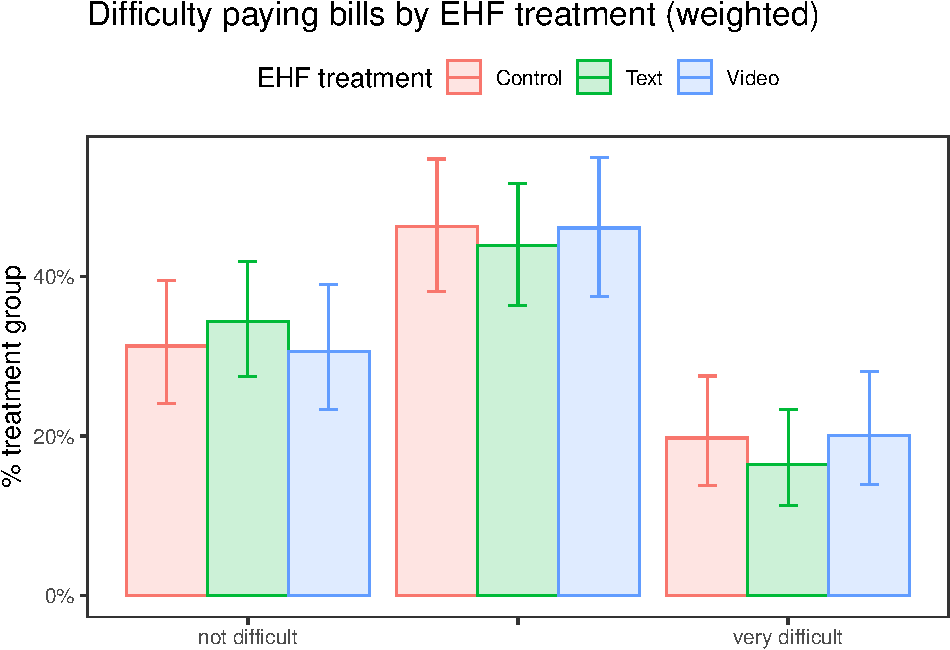
\includegraphics{EHF_Spring2025_files/figure-latex/fig-bills-1.pdf}
\newpage

\section{Reporting full covariate results (Home Depot)}\label{app-cov}

\begin{table}
\centering
\caption{\label{tab:tab-app-full-cov}Full covariate reporting for all OLS estimates \textbackslash{}label\{tab:tab-app-full-cov\}}
\centering
\begin{threeparttable}
\begin{tabular}[t]{lccccc}
\toprule
  & Fin. security & Coworker loyal & Emp. loyal & Emp. reco. & UI support\\
\midrule
(Intercept) & \num{0.531}** & \num{0.577}** & \num{0.423}** & \num{0.629}** & \num{0.492}**\\
 & (\num{0.129}) & (\num{0.108}) & (\num{0.126}) & (\num{0.122}) & (\num{0.136})\\
HDTreatmenttxt & \num{0.043} & \num{0.097}$^+$ & \num{0.008} & \num{-0.020} & \num{-0.055}\\
 & (\num{0.064}) & (\num{0.055}) & (\num{0.061}) & (\num{0.065}) & (\num{0.063})\\
HDTreatmentvid & \num{-0.067} & \num{0.148}* & \num{0.094} & \num{0.126}* & \num{0.033}\\
 & (\num{0.069}) & (\num{0.058}) & (\num{0.062}) & (\num{0.062}) & (\num{0.059})\\
EHF\_aware\_listTRUE & \num{0.203}** & \num{0.215}** & \num{0.164}** & \num{0.179}** & \num{-0.102}$^+$\\
 & (\num{0.058}) & (\num{0.049}) & (\num{0.057}) & (\num{0.059}) & (\num{0.056})\\
rk\_age & \num{0.004}** & \num{0.002}** & \num{0.005}** & \num{0.004}** & \num{-0.002}*\\
 & (\num{0.001}) & (\num{0.001}) & (\num{0.001}) & (\num{0.001}) & \vphantom{1} (\num{0.001})\\
maleTRUE & \num{0.136}** & \num{-0.042} & \num{-0.077}** & \num{-0.046} & \num{-0.047}\\
 & (\num{0.033}) & (\num{0.026}) & (\num{0.028}) & (\num{0.029}) & (\num{0.031})\\
main\_jobTRUE & \num{-0.116}* & \num{0.008} & \num{0.055} & \num{0.006} & \num{0.002}\\
 & (\num{0.051}) & (\num{0.049}) & (\num{0.054}) & (\num{0.052}) & (\num{0.052})\\
tenure\_num & \num{-0.001} & \num{0.001} & \num{0.001} & \num{0.001} & \num{0.000}\\
 & (\num{0.001}) & (\num{0.001}) & (\num{0.001}) & (\num{0.001}) & (\num{0.001})\\
nonwhiteTRUE & \num{-0.034} & \num{0.034} & \num{0.015} & \num{0.004} & \num{0.178}**\\
 & (\num{0.038}) & (\num{0.029}) & (\num{0.034}) & (\num{0.034}) & (\num{0.035})\\
fulltimeTRUE & \num{-0.008} & \num{0.012} & \num{-0.012} & \num{-0.083}* & \num{0.047}\\
 & (\num{0.039}) & (\num{0.029}) & (\num{0.034}) & (\num{0.034}) & (\num{0.035})\\
hourlyTRUE & \num{-0.097} & \num{-0.121} & \num{-0.115} & \num{-0.143} & \num{0.130}\\
 & (\num{0.091}) & (\num{0.074}) & (\num{0.094}) & (\num{0.091}) & (\num{0.109})\\
collegeTRUE & \num{0.026} & \num{-0.003} & \num{-0.080}* & \num{-0.044} & \num{0.062}\\
 & (\num{0.038}) & (\num{0.032}) & (\num{0.036}) & (\num{0.035}) & (\num{0.039})\\
HDTreatmenttxt × EHF\_aware\_listTRUE & \num{-0.076} & \num{-0.173}** & \num{-0.026} & \num{0.028} & \num{0.149}$^+$\\
 & (\num{0.079}) & (\num{0.067}) & (\num{0.075}) & (\num{0.078}) & (\num{0.078})\\
HDTreatmentvid × EHF\_aware\_listTRUE & \num{0.031} & \num{-0.116}$^+$ & \num{-0.028} & \num{-0.068} & \num{0.116}\\
 & (\num{0.084}) & (\num{0.067}) & (\num{0.076}) & (\num{0.076}) & (\num{0.077})\\
\midrule
\$N\$ & \num{509} & \num{508} & \num{502} & \num{508} & \num{506}\\
\$R\textasciicircum{}2\$ & \num{0.15} & \num{0.11} & \num{0.16} & \num{0.14} & \num{0.09}\\
\$F\$ & \num{8.14} & \num{4.89} & \num{7.83} & \num{6.10} & \num{3.97}\\
\bottomrule
\end{tabular}
\begin{tablenotes}
\item $textasciicircum{}+$ p $<$ 0.1, * p $<$ 0.05, ** p $<$ 0.01 Robust standard errors in parentheses
\end{tablenotes}
\end{threeparttable}
\end{table}

\begin{table}
\centering
\caption{\label{tab:tab-app-full-cov}Full covariate reporting for MNL model \textbackslash{}label\{tab:tab-app-full-cov-mnl\}}
\centering
\begin{threeparttable}
\begin{tabular}[t]{llcc}
\toprule
\multicolumn{2}{c}{ } & \multicolumn{2}{c}{(1)} \\
\cmidrule(l{3pt}r{3pt}){3-4}
  & response & Est. & S.E.\\
\midrule
(Intercept) & Against the union & \num{-1.586}* & \num{0.633}\\
 & Not sure & \num{-0.749} & \num{0.646}\\
HDTreatmenttxt & Against the union & \num{0.458} & \num{0.428}\\
 & Not sure & \num{0.662} & \num{0.443}\\
HDTreatmentvid & Against the union & \num{1.018}* & \num{0.499}\\
 & Not sure & \num{1.312}** & \num{0.505}\\
EHF\_aware\_listTRUE & Against the union & \num{1.244}** & \num{0.424}\\
 & Not sure & \num{0.941}* & \num{0.456}\\
rk\_age & Against the union & \num{0.025}** & \num{0.008}\\
 & Not sure & \num{0.014}$^+$ & \num{0.008}\\
maleTRUE & Against the union & \num{-0.018} & \num{0.255}\\
 & Not sure & \num{-0.457}$^+$ & \num{0.266}\\
main\_jobTRUE & Against the union & \num{0.305} & \num{0.446}\\
 & Not sure & \num{0.508} & \num{0.472}\\
tenure\_num & Against the union & \num{0.020}$^+$ & \num{0.011}\\
 & Not sure & \num{0.001} & \num{0.011}\\
nonwhiteTRUE & Against the union & \num{-0.557}$^+$ & \num{0.303}\\
 & Not sure & \num{0.109} & \num{0.301}\\
fulltimeTRUE & Against the union & \num{-0.320} & \num{0.296}\\
 & Not sure & \num{-0.678}* & \num{0.301}\\
collegeTRUE & Against the union & \num{-0.387} & \num{0.297}\\
 & Not sure & \num{-0.475} & \num{0.334}\\
HDTreatmenttxt × EHF\_aware\_listTRUE & Against the union & \num{-0.685} & \num{0.573}\\
 & Not sure & \num{-0.940} & \num{0.614}\\
HDTreatmentvid × EHF\_aware\_listTRUE & Against the union & \num{-1.247}$^+$ & \num{0.656}\\
 & Not sure & \num{-1.010} & \num{0.677}\\
\midrule
\$N\$ &  & \num{508} & \\
AIC &  & \num{1044} & \\
\bottomrule
\end{tabular}
\begin{tablenotes}
\item $textasciicircum{}+$ p $<$ 0.1, * p $<$ 0.05, ** p $<$ 0.01 Reference category is 'for the union.' Standard errors in parentheses
\end{tablenotes}
\end{threeparttable}
\end{table}

\newpage

\section{Ordered logistic regression models (Home Depot)}\label{app-ol}

\begin{table}
\centering
\caption{\label{tab:tab-app-ol}Ordered logit versions of key regression models \label{tab:tab-app-ol}}
\centering
\begin{tabular}[t]{lccccc}
\toprule
  & Fin. security & Coworker loyal & Emp. loyal & Emp. reco. & UI support\\
\midrule
Text treatment & \num{0.142} & \num{0.587}$^+$ & \num{0.085} & \num{-0.191} & \num{-0.297}\\
 & (\num{0.306}) & (\num{0.316}) & (\num{0.313}) & (\num{0.311}) & (\num{0.312})\\
Video treatment & \num{-0.248} & \num{1.069}** & \num{0.624}$^+$ & \num{0.520} & \num{0.092}\\
 & (\num{0.327}) & (\num{0.345}) & (\num{0.337}) & (\num{0.328}) & (\num{0.319})\\
Pre-exposed & \num{1.079}** & \num{1.419}** & \num{1.044}** & \num{0.987}** & \num{-0.583}*\\
 & (\num{0.299}) & (\num{0.308}) & (\num{0.308}) & (\num{0.310}) & (\num{0.291})\\
Text x pre-exposed & \num{-0.395} & \num{-1.072}** & \num{-0.281} & \num{0.174} & \num{0.738}$^+$\\
 & (\num{0.399}) & (\num{0.409}) & (\num{0.403}) & (\num{0.410}) & (\num{0.397})\\
Video x pre-exposed & \num{-0.140} & \num{-0.811}$^+$ & \num{-0.229} & \num{-0.221} & \num{0.742}$^+$\\
 & (\num{0.424}) & (\num{0.445}) & (\num{0.437}) & (\num{0.437}) & (\num{0.414})\\
\midrule
$N$ & \num{515} & \num{514} & \num{508} & \num{514} & \num{511}\\
AIC & \num{1320} & \num{1140} & \num{1253} & \num{1313} & \num{1390}\\
\bottomrule
\multicolumn{6}{l}{\rule{0pt}{1em}$^+$ p $<$ 0.1, * p $<$ 0.05, ** p $<$ 0.01}\\
\multicolumn{6}{l}{\rule{0pt}{1em}Standard errors in parentheses}\\
\end{tabular}
\end{table}

\newpage

\section{Placebos for UI support (Home Depot)}\label{app-placebo}

\begin{table}
\centering
\begin{talltblr}[         %% tabularray outer open
caption={Support for other social policies, OLS regression  \textbackslash{}label\{tab:tab-placebo\}},
note{}={* p \num{< 0.05}, ** p \num{< 0.01}},
note{ }={Robust standard errors in parentheses.},
]                     %% tabularray outer close
{                     %% tabularray inner open
colspec={Q[]Q[]Q[]},
column{2,3}={}{halign=c,},
column{1}={}{halign=l,},
hline{12}={1,2,3}{solid, black, 0.05em},
}                     %% tabularray inner close
\toprule
& Pension & Childcare \\ \midrule %% TinyTableHeader
Text treatment & \num{-0.031} & \num{-0.028} \\
& (\num{0.060}) & (\num{0.066}) \\
Video treatment & \num{0.052} & \num{-0.031} \\
& (\num{0.057}) & (\num{0.068}) \\
Pre-exposed & \num{0.007} & \num{-0.028} \\
& (\num{0.055}) & (\num{0.061}) \\
Text x pre-exposed & \num{0.022} & \num{0.076} \\
& (\num{0.074}) & (\num{0.082}) \\
Video x pre-exposed & \num{-0.013} & \num{0.133} \\
& (\num{0.073}) & (\num{0.085}) \\
\$N\$ & \num{508} & \num{507} \\
\$R\textasciicircum{}2\$ & \num{0.01} & \num{0.01} \\
\$F\$ & \num{0.76} & \num{1.25} \\
\bottomrule
\end{talltblr}
\end{table}

\newpage

\section{Manipulation check for Walmart experiment}\label{app-manip-wmt}

\begin{table}
\centering
\caption{\label{tab:setup}OLS regression of treatment on correctly reporting a Walmart EHF (manipulation check) \label{tab:tab-manip-check}}
\centering
\begin{tabular}[t]{lcccccccc}
\toprule
  & binary & detailed & binary  & detailed  & binary   & detailed   & binary    & detailed   \\
\midrule
treated & \num{0.115}** &  & \num{0.095}** &  & \num{0.118}** &  & \num{0.103}** & \\
 & (\num{0.028}) &  & (\num{0.027}) &  & (\num{0.029}) &  & (\num{0.028}) & \\
placebo &  & \num{-0.042} &  & \num{-0.013} &  & \num{-0.061} &  & \num{-0.027}\\
 &  & (\num{0.035}) &  & (\num{0.031}) &  & (\num{0.037}) &  & (\num{0.032})\\
charity treatment &  & \num{0.104}** &  & \num{0.060} &  & \num{0.097}* &  & \num{0.067}\\
 &  & (\num{0.039}) &  & (\num{0.037}) &  & (\num{0.041}) &  & (\num{0.040})\\
solidarity treatment &  & \num{0.085}* &  & \num{0.114}** &  & \num{0.079} &  & \num{0.111}**\\
 &  & (\num{0.039}) &  & (\num{0.040}) &  & (\num{0.042}) &  & (\num{0.042})\\
treat x pre-exposed &  &  & \num{0.087} &  &  &  & \num{0.073} & \\
 &  &  & (\num{0.055}) &  &  &  & (\num{0.058}) & \\
placebo x pre-exposed &  &  &  & \num{-0.025} &  &  &  & \num{-0.028}\\
 &  &  &  & (\num{0.072}) &  &  &  & (\num{0.076})\\
charity x pre-exposed &  &  &  & \num{0.139} &  &  &  & \num{0.135}\\
 &  &  &  & (\num{0.075}) &  &  &  & (\num{0.079})\\
solidarity x pre-exposed &  &  &  & \num{0.006} &  &  &  & \num{-0.015}\\
 &  &  &  & (\num{0.080}) &  &  &  & (\num{0.083})\\
\midrule
Sample & full & full & full & full & high quality & high quality & high quality & high quality\\
$N$ & \num{1078} & \num{1078} & \num{1078} & \num{1078} & \num{980} & \num{980} & \num{980} & \num{980}\\
\bottomrule
\multicolumn{9}{l}{\rule{0pt}{1em}* p $<$ 0.05, ** p $<$ 0.01}\\
\multicolumn{9}{l}{\rule{0pt}{1em}Robust standard errors in parentheses.}\\
\end{tabular}
\end{table}

\end{document}
